\chapter{基于微分平坦的直升机协同吊挂系统实时避障轨迹规划}
段登燕  祖瑞  余天乐  赵林  李建波
\section{摘要}
为解决直升机协同吊挂系统避障轨迹规划时状态量多、约束复杂导致的收敛性差、实时性不佳等问题,提出了基于微分平坦和MINCO(Control effort minimizer)轨迹表示方法的实时避障轨迹规划方法。首先,分析了直升机协同吊挂系统的微分平坦特性,给出了考虑吊索力的直升机微分平坦输出,详细推导了吊挂物建模为质点和刚体两种情况下协同吊挂系统的微分平坦特性。接着,基于MINCO轨迹及其时空形变方法,将直升机协同吊挂避障问题转换为无约束优化问题处理。以协同吊挂系统的微分平坦输出和分段时间为优化变量,以最小化微分平坦输出轨迹能量和总时间为目的,将吊挂物避障、吊挂物状态量可行性、直升机避障、直升机间避免相互碰撞、吊索避障、吊索力可行性等约束作为惩罚函数来处理,给出了吊挂物建模为质点和刚体两种情况下协同吊挂系统的避障优化方法。最后,以四个小型直升机协同吊挂为例,在随机生成的多个地图上随机指定目标点,仿真验证了本文提出的协同吊挂系统避障优化方法的实时性、有效性和可行性。

\section{引言}

直升机能垂直起降、定点悬停,可以到达其他机型难以到达的区域,且其独特的外挂吊运方式使得直升机运送货物时不受机舱容积、货物体积的限制,具有鲜明的优势。但单个直升机的载重是有限的,相比研制重型直升机的成本和周期,多直升机协同吊挂可以充分利用现有直升机,更具可行性\cite{meier1988efficient,curtiss1985stability, bernard2011autonomous}。同时,直升机协同吊挂带来的复杂多体动力学问题使得协同吊挂系统状态量更多、耦合性更强,相比单机吊挂更有复杂性和挑战性\cite{li2014coordinated, enciu2017flight, berrios2019flight, duan2022optimal}。近年来,随着无人机的兴起尤其是四轴无人机成本低、操作简单,越来越多的研究开始针对无人机带吊挂的建模、控制和轨迹规划问题\cite{gassner2017dynamic, geng2020control, jin2022adaptive},这也给直升机外挂运输问题的研究提供了新思路。本文主要针对协同吊挂系统状态量多、约束复杂造成的轨迹规划时收敛性差、实时性不佳问题,考虑直升机特性,提出一种直升机协同吊挂实时避障轨迹规划方法。

关于协同吊挂系统的轨迹规划,
Salinas等\cite{salinas2018null}针对一直升机协同吊挂系统,考虑质点吊挂物、柔性吊索,提出了基于零空间的协同吊挂系统路径跟随控制策略,该方法考虑了避障、负载分配和队形变换等需求,但没有考虑系统的动力学约束。
Hegde\cite{hegde2021multi}针对双无人机协同吊挂系统,提出了基于控制障碍函数的避障策略,但难以推广到更多无人机协同吊挂的情况,且该方法中两个无人机间的距离是固定的、不支持形变。
Arab\cite{arab2021planning}针对多无人机协同吊挂系统,提出了一种基于改进快速扩展随机树算法的避障策略,但该方法既不支持队形改变,也没有考虑系统的动力学关系。
Aliyu\cite{aliyu2022control}针对一双无人机带吊挂系统,提出了基于改进人工势能场避障方法的神经网络图论分布式位置控制,但文中只考虑了两个无人机的避障,没有考虑吊挂物和绳索的避障。
可见,现有文献中的避障方法大多没有考虑协同吊挂系统的动力学关系,而协同吊挂系统中吊挂物运动是由直升机运动实现的,不考虑动力学关系很有可能导致为直升机和吊挂物规划出来的路径不能同时满足的情况。
Jackson等\cite{jackson2020scalable}针对无人机协同吊挂系统,将吊挂物建模为质点并充分利用系统特性,基于ALTRO(Augmented Lagrangian TRajectory Optimizer)\cite{howell2019altro}和ADMM(Alternating Direction Method of Multiplier)提出了一种既可以处理系统非线性动力学和非凸约束又支持分布式并行计算的轨迹优化方法,但轨迹总时间是固定的,仿真和试验中轨迹优化也不是在线进行的,也不涉及地图的实时更新。同时,从文献\cite{jackson2020scalable}可以看出,动力学约束的加入会大大增加避障优化的难度。

基于微分平坦输出开展轨迹规划,可以隐形地考虑协同吊挂系统的动力学约束,也不会增加避障优化问题的难度。Sreenath团队\cite{sreenath2013trajectory, sreenath2013dynamics, wu2014geometric, kotaru2018differential}针对协同吊挂系统的微分平坦特性做了较多研究。文献\cite{sreenath2013dynamics}针对多轴无人机协同吊挂系统,将吊索看作刚性的,分吊挂物建模为质点、刚体两种情况,给出了系统的微分平坦输出。文献\cite{kotaru2018differential}将柔性吊索建模为由弹簧阻尼系统连接的多个质点,给出了柔性吊索多轴无人机协同吊挂的微分平坦输出。在此基础上,相关文献\cite{sreenath2013trajectory, sreenath2013dynamics, wu2014geometric, kotaru2018differential, valentim2019multi}基于微分平坦输出开展了轨迹规划和控制研究。Tang等\cite{tang2015mixed}、Zeng\cite{zeng2020differential}基于微分平坦对单无人机带吊挂系统进行了避障轨迹规划,但鲜有文献涉及多机协同吊挂系统的避障问题。此外,对直升机协同吊挂系统而言,直升机旋翼的入流、挥舞特性使其相比多轴无人机动力学特性更复杂,要获得直升机协同吊挂系统的微分平坦特性,需要做更多的假设。针对直升机的微分平坦特性,Koo等\cite{koo1999differential}假设旋翼挥舞、尾桨力可以忽略不急,基于微分平坦率先设计了直升机控制律。基于类似的假设,Raptis等\cite{raptis2011linear}开展了小型直升机的跟随控制,Zhao\cite{zhao2021differential}等开展了小型直升机的着舰研究。

关于基于微分平坦的轨迹规划,Janson等\cite{janson2015fast}、Gammell\cite{gammell2018informed}等提出了基于采样点的轨迹规划方法。Mellinger等\cite{mellinger2011minimum}采用固定时长的样条来表征无人机的平坦轨迹,Tordesillas等\cite{tordesillas2019faster}基于Bezier样条曲线来表示轨迹规划中的控制点约束。但无论是基于分配点或基于样条的轨迹规划方法,都无法避免因为精细时间离散带来的巨量变量、约束和算力需求。近期,Wang\cite{wang2022geometrically}提出了以最优性充要条件为依据进行时空参数化的MINCO(Minimum Control Effort)轨迹,并且给出了在用户自定义的代价函数下进行时空形变的求解方案。该轨迹简单易用,轨迹计算和代价函数梯度求解均是线性的,运算效率高。基于MINCO轨迹,Quan\cite{quan2022distributed}开展了密集环境下编队飞行的分布式轨迹规划,Ji\cite{ji2022real}开展了无人机空中栖息的实时轨迹规划,均取得了不错的效果。考虑到收敛性、实时性要求,本文基于MINCO开展直升机协同吊挂系统的避障轨迹规划。

在上述基础上,本文提出了基于微分平坦和MINCO轨迹的直升机协同吊挂系统实时避障轨迹规划方案。论文结构如下。第\ref{flatness_total}节分吊挂物建模为质点、刚体两种情况,分析了直升机协同吊挂系统的微分平坦特性,给出了微分平坦映射。第\ref{minco_multilift}节提出了基于MINCO的直升机协同吊挂系统避障轨迹优化方法。第\ref{Section6:simulation}节以四个小型直升机协同吊挂为例,分吊挂物建模为质点和刚体两种情况开展了避障仿真。第\ref{Section6:conclusion}节是总结。

\begin{figure}
    \centering
    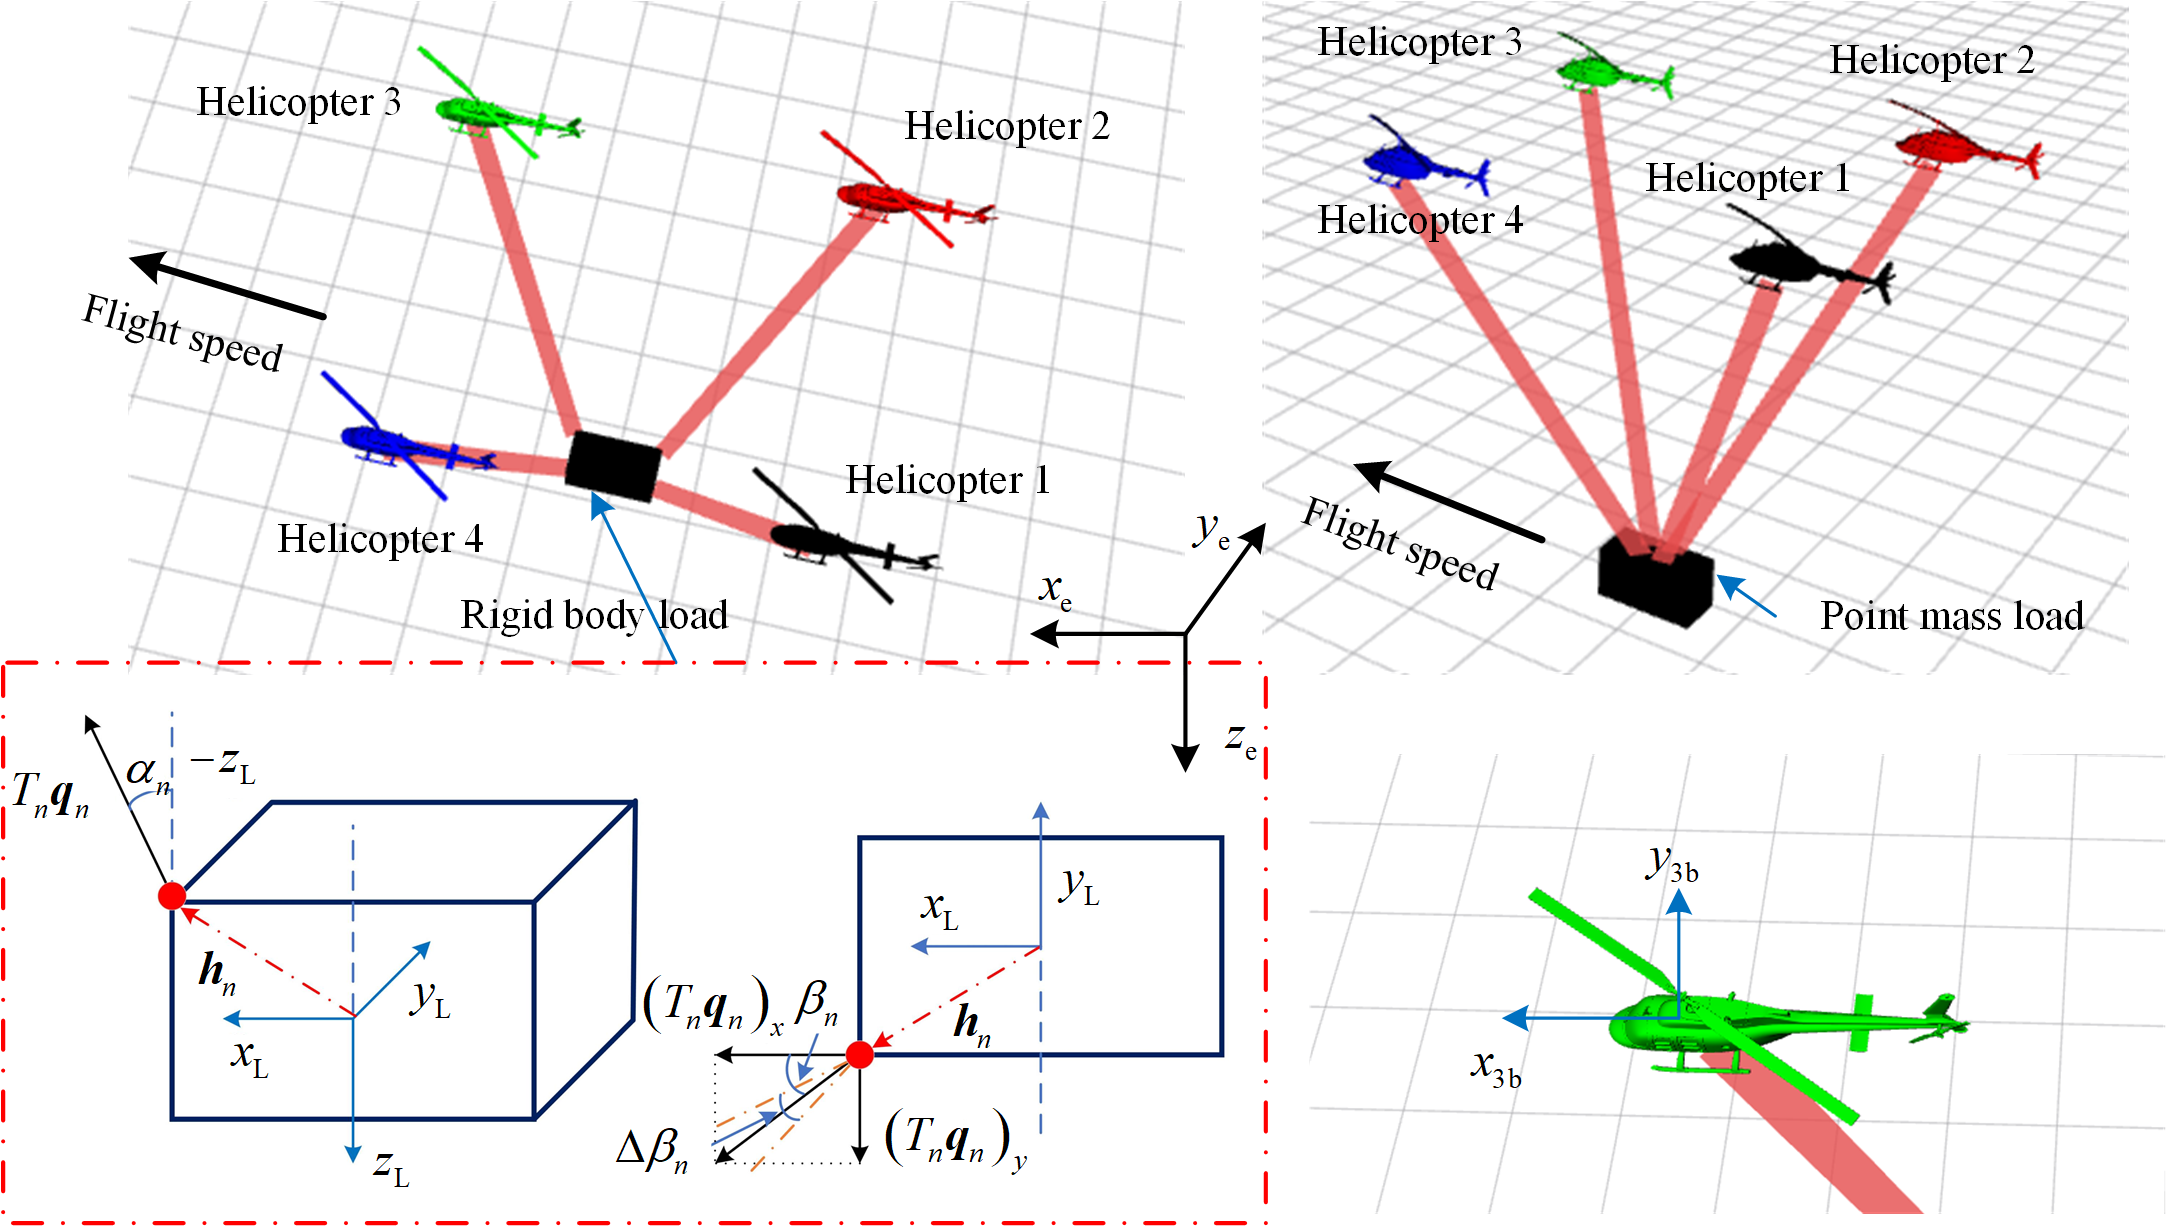
\includegraphics[width = 0.9\textwidth]{fig/figure_chap6/chap6_coordinates.png}
    \caption{吊挂物建模为刚体和质点两种情况下的直升机协同吊挂系统\label{figure6:coordinates}}
\end{figure}

以四直升机协同吊挂为例,图\ref{figure6:coordinates}给出了吊挂物建模为刚体和质点两种情况下的协同吊挂系统。图中,$x_{\rm{e}}y_{\rm{e}}z_{\rm{e}}$为地轴系,其中,$x_{\rm{e}}$指向北,$y_{\rm{e}}$指向东,$z_{\rm{e}}$指向地;$x_{\rm{L}}y_{\rm{L}}z_{\rm{L}}$为吊挂物体轴系,其中,$x_{\rm{L}}$在吊挂物纵向平面内指向前,$z_{\rm{L}}$在吊挂物纵向平面内指向下,$y_{\rm{L}}$可由右手法则得到,原点位于吊挂物重心处;$x_{n\rm{b}}y_{n\rm{b}}z_{n,\rm{b}}$为直升机$n$的体轴系,其中,$x_{n\rm{b}}$在直升机$n$纵向平面内指向前,$z_{n,\rm{b}}$在直升机$n$纵向平面内指向下,$y_{n\rm{b}}$可由右手法则得到,原点位于直升机$n$重心处;$\boldsymbol{h}_n$是从吊挂物重心指向第$n$个吊挂点的向量在吊挂物体轴系中的表示;$T_n\boldsymbol{q}_n$为吊索$n$上的力,$\alpha_n$为$T_n\boldsymbol{q}_n$与$-z_{\rm{L}}$轴的夹角,$\beta_n$为$T_n\boldsymbol{q}_n$在$x_{\rm{L}}y_{\rm{L}}$平面的投影与$x_{\rm{L}}$轴的夹角。

\section{直升机协同吊挂系统微分平坦分析}\label{flatness_total}
\textbf{定义1}微分平坦系统\cite{murray1995differential}:对于一个系统$\dot{\boldsymbol{x}} = f(\boldsymbol{x},\boldsymbol{u})$,$\boldsymbol{x}\in \mathbb{R}^n$,$\boldsymbol{u} \in \mathbb{R}^l$,若存在一组输出$\boldsymbol{z} \in \mathbb{R}^m$,定义$\boldsymbol{z}^{[s]} = [\boldsymbol{z}, \dot{\boldsymbol{z}}, \cdots, \boldsymbol{z}^{(s)}]$为$z$到其$s$阶导数的堆叠,且满足$({\boldsymbol{x}}, {\boldsymbol{u}}) = \Psi({\boldsymbol{z}}^{[s]})$,其中$\Psi$为一代数过程,则系统是微分平坦的,对应的微分平坦输出为$\boldsymbol{z}$。

本节针对吊挂物建模为质点、刚体两种情况,分析直升机协同吊挂系统的微分平坦特性,给出相应的微分平坦输出和微分平坦映射,为第\ref{minco_multilift}节提出以微分平坦输出为优化变量的实时避障优化问题打下基础。系统假设如下:
\begin{enumerate}
    \item  吊索质量、阻力忽略不计;
    \item  吊索是刚性的且只提供张力;
    \item  忽略吊索自身的旋转;
    \item  吊挂物气动阻力忽略不计;
    \item  直升机上的吊挂点位于重心处;
    \item  其余直升机相关的假设详见\ref{heli_flatness}小节。
\end{enumerate}

需要说明的是,直升机协同吊挂系统实时避障问题的研究中,为保证飞行安全性、优化问题收敛性、地图更新的实时性,系统飞行速度较小。因此假设吊挂物气动阻力、各直升机机身气动阻力忽略不计是合理的。

\subsection{直升机的微分平坦特性\label{heli_flatness}}
考虑直升机的状态变量为$\boldsymbol{x} = [\boldsymbol{r}{\rm{^T}}, \boldsymbol{v}{\rm{^T}},\boldsymbol{R}{\rm{^T}}, \boldsymbol{\omega}{\rm{^T}}]\rm{^T}$,其中$ \boldsymbol{r} \in \mathbb{R}^3$为地轴系下的重心位置,$\boldsymbol{v} \in \mathbb{R}^3$为地轴下的平动速度,$\boldsymbol{R}\in SO(3)$为机身姿态,$\boldsymbol{\omega} \in \mathbb{R}^3$为机体角速度。直升机控制输入为$\boldsymbol{u}$,直升机上所有动力部件(单旋翼带尾桨直升机为主旋翼和尾桨,纵列式直升机为前后两个旋翼)相对重心在体轴系下产生的合力、合力矩表示为${\boldsymbol{F}\rm{_{A1}}}(\boldsymbol{x}, \boldsymbol{u})$、${\boldsymbol{M}\rm{_{A1}}}(\boldsymbol{x}, \boldsymbol{u})$,其他气动部件相对重心在体轴系产生的力和力矩为${\boldsymbol{F}\rm{_{A2}}}(\boldsymbol{x})$、${\boldsymbol{M}\rm{_{A2}}}(\boldsymbol{x})$。吊索施加在直升机上的力及其相对重心的力矩在地轴系下为$\boldsymbol{F}\rm{_C}$、$\boldsymbol{M}\rm{_C}$,那么直升机的动力学方程可以由如下微分方程描述:
\begin{subnumcases} {\label{eq_dynamics} }
    \dot{ \boldsymbol{r} }= \boldsymbol{v} \label{eq_dynamics_a}\\
    m\dot{ \boldsymbol{v}} = mg\boldsymbol{e}_3 + {\boldsymbol{F}\rm{_C}}+  {\boldsymbol{RF}\rm{_{A1}}}(\boldsymbol{x},\boldsymbol{u}) + {\boldsymbol{RF}\rm{_{A2}}}(\boldsymbol{x})\label{eq_dynamic_b} \\
    \dot{\boldsymbol{R}} = \boldsymbol{R}\hat{\boldsymbol{\omega}} \label{eq_dynamics_c}\\
    \boldsymbol{J\dot{\omega}} = - \boldsymbol{\omega} \times \boldsymbol{J\omega} + \boldsymbol{R}{\rm{^T}}{\boldsymbol{M}\rm{_C}} + {\boldsymbol{M}\rm{_{A1}}}(\boldsymbol{x}, \boldsymbol{u}) + {\boldsymbol{M}\rm{_{A2}}}(\boldsymbol{x})\label{eq_dynamics_d}
\end{subnumcases}

其中,$m \in \mathbb{R}_{\ge 0}$代表直升机质量,$\boldsymbol{e}_i \in \mathbb{R}^3$为第$i$个元素为1的单位向量,$g$为重力加速度,$J$为以重心为原点关于机体轴系的惯量张量矩阵,$\hat{\left( \cdot \right)}$为向量$\left( \cdot \right)$的反对称矩阵。

假设吊索力、力矩及其高阶导数已知,以位置和偏航角作为直升机的微分平坦输出${\boldsymbol{z}} = [\boldsymbol{r}, \psi]$。下面详细给出考虑吊索力的直升机微分平坦相关假设及变换过程。

首先对直升机的线运动即式\ref{eq_dynamic_b}做如下假设:
\begin{enumerate}
    \item  假设旋翼产生的后向力和侧向力相对旋翼拉力很小,可以忽略不计;
    \item  若为单旋翼带尾桨直升机,假设尾桨拉力相对旋翼拉力很小,可以忽略不计;
    \item  忽略旋翼的挥舞运动,旋翼拉力垂直桨毂平面指向上;
    \item  假设旋翼轴前倾角为0,即桨毂平面与直升机体轴系$x-y$平面平行;
    \item  忽略机身阻力及其他部件的气动力,即${\boldsymbol{F}\rm{_{A2}}}(\boldsymbol{x}) = \boldsymbol{0}$。
\end{enumerate}

经过以上假设(1)-(4),可知${\boldsymbol{F}\rm{_{A1}}}(\boldsymbol{x}, \boldsymbol{u}) = [ 0, 0, -T]\rm{^T}$,其中$T$为旋翼总拉力。进一步,式\ref{eq_dynamic_b}可以简化为:
\begin{equation}\label{eq_dynamic_b_simplify}
    m\dot{ \boldsymbol{v}} = mg\boldsymbol{e}_3 + {\boldsymbol{F}\rm{_C}}+  {\boldsymbol{R}}{[0, 0, -T]\rm{^T}} 
\end{equation}

将式\ref{eq_dynamic_b_simplify}同机体坐标系在地轴系下的投影${\boldsymbol{x}\rm{_b}} = \boldsymbol{Re_1}$和${\boldsymbol{y}\rm{_b}} = \boldsymbol{Re_2} $分别做点积可得
\begin{equation}
    {(\boldsymbol{Re}_i)\rm{^T}}(\dot{\boldsymbol{v}} -g{\boldsymbol{e_3}} - \frac{1}{m}{\boldsymbol{F}\rm{_C}}) = 0 \,\,\,\, \forall i \in \left\{ {1,2} \right\}
\end{equation}

由旋翼拉力$T$的非负性及其方向同${\boldsymbol{z}\rm{_b}} = \boldsymbol{Re_3}$在任何情况下相反可得,
\begin{equation}\label{z_b}
    {\boldsymbol{z}\rm{_b}} = \mathcal{N} (\dot{\boldsymbol{v}} -g{\boldsymbol{e_3}} - \frac{1}{m}{\boldsymbol{F}\rm{_C}})
\end{equation}
其中,$\mathcal{N}(\boldsymbol{x}) = \frac{\boldsymbol{x}}{\left\| {\boldsymbol{x}} \right\|_2}$。

将式\ref{eq_dynamic_b_simplify}与$\boldsymbol{z}_b = \boldsymbol{R}\boldsymbol{e}_3$点积可得
\begin{equation}
    T = -{\boldsymbol{z}\rm{_b^T}} (m\dot{\boldsymbol{v}}  -mg{\boldsymbol{e_3}} - {\boldsymbol{F}\rm{_C}})
\end{equation}

接下来基于Hopf纤维化定义下的偏航角和倾斜角来恢复出整个机身姿态。现已知机身$\boldsymbol{z}\rm{_b}$轴由式\ref{z_b}给出,偏航角由微分平坦输出给出,则对应的偏航四元数为
\begin{equation}
    \boldsymbol{q}_\psi = [\cos(\psi/2), 0, 0, \sin(\psi/2)]\rm{^T}
\end{equation}

将机身$z$轴从$\boldsymbol{e}_3$转换到$\boldsymbol{z}\rm{_b}$的倾斜四元数为
\begin{equation}
    \boldsymbol{q}_z = \frac{1}{\sqrt{2(1+{\boldsymbol{z}\rm{_b}}(3))}}(1+{\boldsymbol{z}\rm{_b}}(3), -{\boldsymbol{z}\rm{_b}}(2), {\boldsymbol{z}\rm{_b}}(1), 0)\rm{^T}
\end{equation}

可以验证,$\boldsymbol{q}_z$中不包含任何和偏航有关的旋转分量,那么可得整个直升机的姿态四元数$\boldsymbol{q}$为
\begin{equation}
    \boldsymbol{q} = \boldsymbol{q}_z \otimes \boldsymbol{q}_\psi = \frac{1}{\sqrt{2(1+{\boldsymbol{z}\rm{_b}}(3))}} \left( \begin{array}{c}
        (1+\boldsymbol{z}{\rm{_b}}(3))\cos(\psi/2))\\
        -\boldsymbol{z}{\rm{_b}}(2)\cos(\psi/2) + \boldsymbol{z}{\rm{_b}}(1)\sin(\psi/2)\\
        \boldsymbol{z}{\rm{_b}}(1)\cos(\psi/2) + \boldsymbol{z}{\rm{_b}}(2)\sin(\psi/2)\\
        (1+\boldsymbol{z}{\rm{_b}}(3))\sin(\psi/2)\\
        \end{array} \right)
\end{equation}

四元数$q$对应的姿态矩阵为
\begin{equation}\label{R}
    \boldsymbol{R} = \mathcal{R}{\rm{_{quat}}}(\boldsymbol{q})
\end{equation}

将式\ref{R}代入式\ref{eq_dynamics_c}中,可得
\begin{equation}\label{omega}
    \begin{aligned}
        \boldsymbol{\omega} &= 2(\boldsymbol{q}{\rm{_z}} \otimes \boldsymbol{q}{\rm{_\psi}})^{-1} \otimes (
            \dot{\boldsymbol{q}}{\rm{_z}} \otimes \boldsymbol{q}_\psi + \boldsymbol{q}{\rm{_z}}\otimes{\dot{\boldsymbol{q}}_\psi})\\
            &= \left(\begin{array}{c}
                \dot{\boldsymbol{z}}{\rm{_b}}(1)\sin(\psi) - \dot{\boldsymbol{z}}{\rm{_b}}(2)\cos(\psi) - \dot{\boldsymbol{z}}{\rm{_b}}(3)(\boldsymbol{z}{\rm{_b}}(1)\sin(\psi) - \boldsymbol{z}{\rm{_b}}(2)\cos(\psi))/(1+\boldsymbol{z}{\rm{_b}}(3))\\
                \dot{\boldsymbol{z}}{\rm{_b}}(1)\cos(\psi) + \dot{\boldsymbol{z}}{\rm{_b}}(2)\sin(\psi) - \dot{\boldsymbol{z}}{\rm{_b}}(3)(\boldsymbol{z}{\rm{_b}}(1)\cos(\psi) + \boldsymbol{z}{\rm{_b}}(2)\sin(\psi))/(1+\boldsymbol{z}{\rm{_b}}(3))\\
                (\boldsymbol{z}{\rm{_b}}(2)\dot{\boldsymbol{z}}{\rm{_b}}(1) - \boldsymbol{z}{\rm{_b}}(1)\dot{\boldsymbol{z}}{\rm{_b}}(2))/(1+\boldsymbol{z}{\rm{_b}}(3)) + \dot{\psi}
            \end{array}\right)
    \end{aligned}
\end{equation}
其中,
\begin{equation}
    \dot{\boldsymbol{z}}{\rm{_b}} = \mathcal{DN}(\dot{\boldsymbol{v}} -g{\boldsymbol{e_3}} - \frac{1}{m}{\boldsymbol{F}\rm{_C}}){\rm{^T}}(\ddot{\boldsymbol{v}} - \frac{1}{m} \dot{\boldsymbol{F}}{\rm{_C}} )
\end{equation}
\begin{equation}
    \mathcal{DN}(\boldsymbol{x}) = \frac{1}{\left\| {\boldsymbol{x}} \right\|}(\boldsymbol{I} - \frac{\boldsymbol{xx}{\rm{^T}}}{\boldsymbol{x}{\rm{^T}}\boldsymbol{x}})
\end{equation}
其中,$\boldsymbol{I}\in \mathbb{R}^{3\times3}$为单位矩阵。

可见,假设$\boldsymbol{F}\rm{_C}$和$\dot{\boldsymbol{F}}\rm{_C}$已知,通过$\boldsymbol{r}$、$\dot{\boldsymbol{r}}$、$\boldsymbol{r}{\rm{^{(2)}}}$、$\boldsymbol{r}{\rm{^{(3)}}}$以及$\psi$、$\dot \psi$可以计算出所有状态$\boldsymbol{x} = [\boldsymbol{r}\rm{^T}, \boldsymbol{v}\rm{^T},\boldsymbol{R}\rm{^T}, \boldsymbol{\omega}\rm{^T}]\rm{^T}$和所需的旋翼拉力$T$, 对式\ref{omega}进一步对时间微分,利用$\boldsymbol{r}{\rm{^{(4)}}}$、$\psi ^{(2)}$、$\boldsymbol{F}\rm{_C^{(2)}}$可以得到$\dot \omega$。此外,由假设直升机吊挂点位于重心处可知$\boldsymbol{M}_{\rm{C}} = \boldsymbol{0}$,进而通过式\ref{eq_dynamics_d}可得
\begin{equation}
    \boldsymbol{M}{\rm{_{A1}}}(\boldsymbol{x}, \boldsymbol{u}) = \boldsymbol{J}\dot{\boldsymbol{\omega}} + \boldsymbol{\omega} \times \boldsymbol{J\omega}  - \boldsymbol{M}{\rm{_{A2}}}(x)
\end{equation}

对于如何控制输入$\boldsymbol{u}$产生旋翼拉力$T$和力矩$\boldsymbol{M}{\rm{_{A1}}}$,多种控制方法如动态逆、自抗扰等均能达到目的。至此,给出了考虑吊索拉力的直升机微分平坦变换方法。

\subsection{吊挂物建模为质点时系统的微分平坦输出特性}\label{point_load_flatness}
吊挂物建模为质点时,选择状态变量为$\boldsymbol{x}{\rm{_L}} = [\boldsymbol{r}{\rm{_L^T}}, \boldsymbol{v}{\rm{_L^T}}]{\rm{^T}}$,其中,$\boldsymbol{r}{\rm{_L}}$为地轴系下吊挂物的位置,$\boldsymbol{v}{\rm{_L}}$是地轴系下吊挂物的平动速度。其动力学方程为
\begin{subnumcases}{\label{point_load_dynamics}}
    \dot{\boldsymbol{r}}{\rm{_L}} = \boldsymbol{v}{\rm{_L}} \label{point_load_dynamics_a}\\
    m{\rm{_L}}\dot{\boldsymbol{v}}{\rm{_L}} =  \sum\limits_{n=1}^N {T_n\boldsymbol{q}_n} + m{\rm{_L}}g\boldsymbol{e}_3 \label{point_load_dynamics_b} 
\end{subnumcases}
其中$N$为直升机数量,$\boldsymbol{q}_n$是从吊挂物上吊挂点指向直升机$n$上吊挂点的单位向量在吊挂物体轴系中的表示。

选取吊挂物的微分平坦输出$\boldsymbol{z} = [\boldsymbol{r}{\rm{_L^T}}, (T_2\boldsymbol{q}_2){\rm{^T}}, \cdots, (T_N\boldsymbol{q}_N){\rm{^T}}]$。由式\ref{point_load_dynamics_a}可得$\boldsymbol{v}{\rm{_L}}$,进一步关于时间求导可得$\dot{\boldsymbol{v}}{\rm{_L}}$,进而由式\ref{point_load_dynamics_b}可得$T_1\boldsymbol{q}_1$。此外,$\boldsymbol{q}_n$、$T_n$可以写为
\begin{equation}\label{q_i}
    \boldsymbol{q}_n = \mathcal{D}(T_n\boldsymbol{q}_n) \,\,\,\, \forall \,\, n \in \left\{ 1, 2,\cdots, N\right\}
\end{equation}
\begin{equation}\label{T_i}
    T_n = T_n\boldsymbol{q}_n\cdot\boldsymbol{q}_n \,\,\,\, \forall \,
    \, n \in \left\{1, 2, \cdots, N\right\}
\end{equation}

进一步,由\ref{heli_flatness}节可知,直升机$n$的微分平坦输出为${\boldsymbol{z}_n} = [\boldsymbol{r}_n, \psi_n]$,将$\psi_n$写入系统的微分平坦输出后,要得到直升机$n$的所有状态和控制输入,仍需要得知$\boldsymbol{r}_n$至其四阶导、$\boldsymbol{F}_{{\rm{C}},n}$至其二阶导的值。

假设吊索长度不变,吊挂点位于直升机重心处,对于质点吊挂物,根据运动学关系:
\begin{equation}\label{r_i_k_point}
    \boldsymbol{r}_n^{(k)} = \boldsymbol{r}^{(k)}_{\rm{L}} + L_n \boldsymbol{q}_n^{(k)} \,\,\,\, \forall k \in \left\{ {0,1,\cdots,4} \right\}
\end{equation}
其中,$L_n$是第$n$根吊索的长度。

$\boldsymbol{F}_{{\rm{C}},n}$至其二阶导可以写为:
\begin{equation}
    \boldsymbol{F}_{{\rm{C}},n}^{(k)} = -\left(T_n \boldsymbol{q}_n\right)^{(k)} \,\,\,\, \forall \,\, k \in \left\{0, 1, 2\right\}
\end{equation}

需要注意的是,$T_1\boldsymbol{q}_1$是由微分平坦输出$\boldsymbol{z} = [\boldsymbol{r}{\rm{_L^T}}, (T_2\boldsymbol{q}_2){\rm{^T}}, \cdots, (T_N\boldsymbol{q}_N){\rm{^T}}]$及其高阶导数经式\ref{point_load_dynamics_b}确定的。可以看出,$\left(T_1\boldsymbol{q}_1\right)^{(k)}$与$\boldsymbol{r}_{\rm{L}}^{(k+2)}$、$\left(T_2\boldsymbol{q}_2\right)^{(k)}$、\ldots、$\left(T_N\boldsymbol{q}_N\right)^{(k)}$有关。此外,$\boldsymbol{q}_n$由式\ref{q_i}确定,进而可知式\ref{r_i_k_point}中需要的$\boldsymbol{q}_n^{(k)}$与$(T_n\boldsymbol{q}_n)^{(k)}$有关。

所以,吊挂物建模为质点时,协同吊挂系统的微分平坦输出可以为
\begin{equation}
    \boldsymbol{z} = [\boldsymbol{r}{\rm{_L^T}}, (T_2\boldsymbol{q}_2){\rm{^T}}, \cdots, (T_N\boldsymbol{q}_N){\rm{^T}}, \psi_1, \psi_2, \cdots, \psi_N]
\end{equation}

要想获得系统的全部微分平坦变换,需要$\boldsymbol{r}{\rm{_L}}$的六阶导,$T_2\boldsymbol{q}_2$、\ldots、$T_N\boldsymbol{q}_N$的四阶导,$\psi_n$的二阶导。

\subsection{吊挂物建模为刚体时系统的微分平坦输出特性}\label{rigid_load_flatness}

吊挂物建模为刚体时,选择状态变量为$\boldsymbol{x}{\rm{_L}} = [\boldsymbol{r}{\rm{_L^T}}, \boldsymbol{v}{\rm{_L^T}}, \boldsymbol{R}{\rm{_L^T}}, \boldsymbol{\omega}{\rm{_L^T}}]{\rm{^T}}$,其中$\boldsymbol{R}{\rm{_L}} \in SO(3)$为吊挂物姿态,$\boldsymbol{\omega}{\rm{_L}}$是吊挂物体轴系下的角速度。吊挂物的动力学方程可以写为
\begin{subnumcases}{\label{load_dynamics}}
    \dot{\boldsymbol{r}}{\rm{_L}} = \boldsymbol{v}{\rm{_L}\label{load_dynamics_a}}\\
    m{\rm{_L}}\dot{\boldsymbol{v}}{\rm{_L}} =  \boldsymbol{R}{\rm{_L}}\sum\limits_{n=1}^N {T_n\boldsymbol{q}_n}  + m{\rm{_L}}g\boldsymbol{e}_3  \label{load_dynamics_b}\\
    \dot{\boldsymbol{R}}{\rm{_L}} = \boldsymbol{R}{\rm{_L}}\hat{\boldsymbol{\omega}}{\rm{_L}} \label{load_dynamics_c}\\
    \boldsymbol{J}{\rm{_L}}\dot{\boldsymbol{\omega}}{\rm{_L}} + \boldsymbol{\omega}{\rm{_L}} \times \boldsymbol{J}{\rm{_L}}\boldsymbol{\omega}{\rm{_L}} = \sum\limits_{n=1}^N {\boldsymbol{h}_n \times T_n\boldsymbol{q}_n}  \label{load_dynamics_d}
\end{subnumcases}

首先选择$\boldsymbol{r}{\rm{_L}}$、$\boldsymbol{R}{\rm{_L}}$为吊挂物的微分平坦输出。基于$\boldsymbol{r}{\rm{_L}}$、$\boldsymbol{R}{\rm{_L}}$及其高阶导数,由式\ref{load_dynamics_a}可以确定$\boldsymbol{v}{\rm{_L}}$,进一步求导可以得到$\dot{\boldsymbol{v}}{\rm{_L}}$;由式\ref{load_dynamics_c}可以确定$\boldsymbol{\omega}{\rm{_L}}$,进一步求导可得$\dot{\boldsymbol{\omega}}{\rm{_L}}$。接着,由式\ref{load_dynamics_b}、\ref{load_dynamics_d}可得$\sum\nolimits_{n=1}^{N}{T_n\boldsymbol{q}_n}$和$\sum\nolimits_{n=1}^{N}{\boldsymbol{h}_n \times T_n\boldsymbol{q}_n}$的值,即:
\begin{equation}
    \Phi\left[
        \begin{array}{c}
            T_1\boldsymbol{q}_1\\
            T_2\boldsymbol{q}_2\\
            \vdots\\
            T_N\boldsymbol{q}_N
        \end{array}
    \right] = \left[\begin{array}{c}
        \boldsymbol{R}{\rm{_L^T}}(m_L(\dot{\boldsymbol{v}}{\rm{_L}}-g\boldsymbol{e}_3))\\
        \boldsymbol{J}{\rm{_L}}\dot{\boldsymbol{\omega}}{\rm{_L}} + \boldsymbol{\omega}{\rm{_L}} \times \boldsymbol{J}{\rm{_L}}\boldsymbol{\omega}{\rm{_L}}
    \end{array}
    \right] 
\end{equation}
其中,
\begin{equation}
    \Phi = \left[ {\begin{array}{*{20}{c}}
        {\boldsymbol{I}}&{\boldsymbol{I}}&{\cdots}&{\boldsymbol{I}}\\
        {\hat{\boldsymbol{h}}_1}&{\hat{\boldsymbol{h}}_2}&{\cdots}&{\hat{\boldsymbol{h}}_N}
        \end{array}} \right]
\end{equation}


定义$\Phi^{+}$是$\Phi$的Moore-Penrose广义逆。$\boldsymbol{U}$是以$\Phi$的零空间的基为列向量扩张成的矩阵,可得
\begin{equation}\label{T_each}
    \left[\begin{array}{c}
        T_1\boldsymbol{q}_1\\
        T_2\boldsymbol{q}_2\\
        \vdots\\
        T_N\boldsymbol{q}_N
    \end{array} 
    \right] = \Phi^{+}
        \left[\begin{array}{c}
            \boldsymbol{R}{\rm{_L^T}}(m_L(\dot{\boldsymbol{v}}{\rm{_L}}-g\boldsymbol{e}_3))\\
            \boldsymbol{J}{\rm{_L}}\dot{\boldsymbol{\omega}}{\rm{_L}} + \boldsymbol{\omega}{\rm{_L}} \times \boldsymbol{J}{\rm{_L}}\boldsymbol{\omega}{\rm{_L}}
        \end{array}
        \right]
     + \boldsymbol{U\Lambda}
\end{equation}

其中,$\boldsymbol{\Lambda} \in \mathbb{R}^{3N-6}$。可以看出,若知$\boldsymbol{\Lambda}$及其高阶项,可得$T_n\boldsymbol{q}_n$及其高阶项。因此,将$\boldsymbol{\Lambda}$写入协同吊挂系统的微分平坦输出。

与\ref{point_load_flatness}节类似,将$\psi_n$写入系统的微分平坦输出后,要得到直升机$n$的所有状态和控制输入,仍需要得知$\boldsymbol{r}_n$至其四阶导、$\boldsymbol{F}_{{\rm{C}},n}$至其二阶导的值。

假设直升机上的吊挂点位于其重心上,吊索长度不变,对刚体吊挂物,由运动学关系:
\begin{equation}\label{r_i}
\left\{\begin{aligned}
        \boldsymbol{r}_n &= \boldsymbol{r}{\rm{_L}} + \boldsymbol{R}{\rm{_L}}(\boldsymbol{h}_n+L_n\boldsymbol{q}_n) \\
        \dot{\boldsymbol{r}}_n &= \dot{\boldsymbol{r}}{\rm{_L}} + \dot{\boldsymbol{R}}{\rm{_L}}(\boldsymbol{h}_n + \boldsymbol{L}_n\boldsymbol{q}_n) + \boldsymbol{R}{\rm{_L}}\boldsymbol{L}_n\dot{\boldsymbol{q}}_n\\
        {\boldsymbol{r}}_n^{(2)} &= {\boldsymbol{r}}{\rm{_L^{(2)}}} + {R}{\rm{_L^{(2)}}}(\boldsymbol{h}_n+\boldsymbol{L}_n\boldsymbol{q}_n)+2\dot{\boldsymbol{R}}{\rm{_L}}\boldsymbol{L}_n\boldsymbol{q}_n+\boldsymbol{R}{\rm{_L}}\boldsymbol{L}_n{\boldsymbol{q}}_n^{(2)}\\
        \boldsymbol{r}_n^{(3)} &= \boldsymbol{r}{\rm{_L^{(3)}}} + \boldsymbol{R}{\rm{_L^{(3)}}}(\boldsymbol{h}_n + \boldsymbol{L}_n\boldsymbol{q}_n) + \boldsymbol{R}{\rm{_L^{(2)}}}\boldsymbol{L}_n\dot{\boldsymbol{q}}_n + 2\boldsymbol{R}{\rm{_L^{(2)}}}\boldsymbol{L}_n\boldsymbol{q}_n + 2\dot{\boldsymbol{R}}{\rm{_L}}\boldsymbol{L}_n\dot{\boldsymbol{q}_n} + \dot{\boldsymbol{R}}{\rm{_L}}\boldsymbol{L}_n\boldsymbol{q}_n^{(2)} + \boldsymbol{R}{\rm{_L}}\boldsymbol{L}_n\boldsymbol{q}_n^{(3)}\\
        \boldsymbol{r}{_n^{(4)}} &= \boldsymbol{r}{\rm{_L^{(4)}}} + \boldsymbol{R}{\rm{_L^{(4)}}}(\boldsymbol{h}_n + \boldsymbol{L}_n\boldsymbol{q}_n) + 2\boldsymbol{R}{\rm{_L^{(3)}}}\boldsymbol{L}_n\dot{\boldsymbol{q}}_n + 2\boldsymbol{R}{\rm{_L^{(2)}}}\boldsymbol{L}_n\boldsymbol{q}{_n^{(2)}} + 2\boldsymbol{R}{\rm{_L^{(3)}}}\boldsymbol{L}_n\boldsymbol{q}_n + 4\boldsymbol{R}{\rm{_L^{(2)}}}\boldsymbol{L}_n\dot{\boldsymbol{q}}_n \\
        &+2\dot{R}{\rm{_L}}\boldsymbol{L}_n\boldsymbol{q}{_n^{(2)}} + 2\dot{R}{\rm{_L}}\boldsymbol{L}_n\boldsymbol{q}{_n^{(3)}} + \boldsymbol{R}{\rm{_L}}\boldsymbol{L}_n\boldsymbol{q}_n^{(4)}
    \end{aligned} \right.
\end{equation}

$\boldsymbol{F}_{{\rm{C}},n}$至其二阶导可以写为:
\begin{equation}\label{Fc_i}
    \left\{
        \begin{aligned}
            \boldsymbol{F}_{{\rm{C}},n} &= -\boldsymbol{R}{\rm{_L}}\boldsymbol{T}_n\boldsymbol{q}_n\\
            \boldsymbol{F}^{(1)}_{{\rm{C}},n} &= -\boldsymbol{R}{\rm{_L^{(1)}}}(\boldsymbol{T}_n\boldsymbol{q}_n) - \boldsymbol{R}{\rm{_L}}(\boldsymbol{T}_n\boldsymbol{q}_n)^{(1)}\\
            \boldsymbol{F}^{(2)}_{{\rm{C}},n} &= -\boldsymbol{R}{\rm{_L^{(2)}}}(\boldsymbol{T}_n\boldsymbol{q}_n) - 2\boldsymbol{R}{\rm{_L^{(1)}}}(\boldsymbol{T}_n\boldsymbol{q}_n)^{(1)} - \boldsymbol{R}{\rm{_L}}(\boldsymbol{T}_n\boldsymbol{q}_n)^{(2)}
        \end{aligned}
    \right.
\end{equation}

由式\ref{r_i}、\ref{Fc_i},若想得到$\boldsymbol{r}_n$至其四阶导、$\boldsymbol{F}_{{\rm{C}},n}$至其二阶导的值,需要知道$\boldsymbol{r}{\rm{_L}}$、$\boldsymbol{R}{\rm{_L}}$、$\boldsymbol{q}_n$至其四阶导以及$ T_n \boldsymbol{q}_n$至其二阶导的值。由式\ref{q_i},$\boldsymbol{q}_n$至其四阶导与$T_n\boldsymbol{q}_n$至其四阶导有关。由式\ref{T_each},$T_n\boldsymbol{q}_n$至其四阶导与$\boldsymbol{r}_{\rm{L}}^{(2)}$至$\boldsymbol{r}_{\rm{L}}^{(6)}$、$\boldsymbol{R}_{\rm{L}}$至其四阶导、$\Lambda$至其四阶导、$\boldsymbol{\omega}$至其五阶导有关。再者,由式\ref{load_dynamics_c},$\boldsymbol{\omega}{\rm{_L}}$至其五阶导与$\boldsymbol{R}{\rm{_L}}$至其六阶导有关。

可见,吊挂物建模为刚体时,协同吊挂系统的微分平坦输出可以为
\begin{equation}
    \boldsymbol{z} = [\boldsymbol{r}{\rm{_L^T}}, \boldsymbol{R}{\rm{_L^T}}, \boldsymbol{\Lambda}{\rm{^T}}, \psi_1, \psi_2, \cdots, \psi_N]\rm{^T}
\end{equation}

要想获得系统的微分平坦变换,需要$\boldsymbol{r}{\rm{_L}}$的6阶导、$\boldsymbol{R}{\rm{_L}}$的6阶导、$\boldsymbol{\Lambda}$的四阶导、$\psi_n$的二阶导。

\subsection{简化}
不失一般性,接下来的推导和仿真中,吊挂物无论建模为质点还是刚体,均假设协同吊挂系统中的每个直升机偏航角为0且不变。此外,吊挂物建模为刚体时,为了最小化吊挂物的气动阻力及保证飞行安全,一般要求其姿态角为0且不变。此时,$\boldsymbol{R}_{\rm{L}}$为单位矩阵,其各阶导数均为$\boldsymbol{0}$;$\boldsymbol{\omega}_{\rm{L}}$及其各阶导数均为$\boldsymbol{0}$。

经过上述假设和简化,吊挂物建模为质点时,系统的微分平坦输出变为:
\begin{equation}\label{flatness_point}
    \boldsymbol{z} = [\boldsymbol{r}{\rm{_L^T}}, (T_2\boldsymbol{q}_2){\rm{^T}}, \cdots, (T_n\boldsymbol{q}_n){\rm{^T}}]
\end{equation}

吊挂物建模为刚体时,系统的微分平坦输出变为:
\begin{equation}\label{flatness_rigid}
    \boldsymbol{z} = [\boldsymbol{r}{\rm{_L^T}},  \boldsymbol{\Lambda}{\rm{^T}}]\rm{^T}
\end{equation}

\section{基于MINCO的直升机协同吊挂系统实时避障轨迹优化方法}\label{minco_multilift}
本节基于MINCO轨迹及其时空形变方法\cite{wang2022geometrically},将直升机协同吊挂系统实时避障轨迹规划问题转化为无约束优化问题处理。

\subsection{基于MINCO的轨迹级表示方法}
假设系统的微分平坦输出为$\boldsymbol{z} \in \mathbb{R}^m$,$\boldsymbol{z}^{[s]} = [\boldsymbol{z}, \dot{\boldsymbol{z}}, \cdots, \boldsymbol{z}^{(s)}]$, 考虑如下最小化问题
\begin{equation}\label{optimization_minco}
    \begin{array}{l}
        \mathop {\min }\limits_{\boldsymbol{q}(t)} \int_{{t_0}}^{{t_M}} \boldsymbol{q}(t){\rm{^T}}\boldsymbol{W}\boldsymbol{q}(t){\rm{d}}t\\
        s.t. \,\,\,\, \boldsymbol{z}^{(s)}(t) = \boldsymbol{q}(t),\,\, \forall \,\, t \in [t_0, t_M], \\
        \,\,\,\,\,\,\,\,\,\,\, \boldsymbol{z}^{[s-1]}(t_0) = \bar{\boldsymbol{z}}_0, \,\, \boldsymbol{z}^{[s-1]}(t_M) = \bar{\boldsymbol{z}}_f,\\
        \,\,\,\,\,\,\,\,\,\,\, \boldsymbol{z}^{[d_i-1]}(t_i) = \bar{\boldsymbol{z}}_i, \,\,\,\, 1 \le i  < M\\
        \,\,\,\,\,\,\,\,\,\,\,  t_{i-1} < t_i, \,\,\,\, 1 \le i \le M
    \end{array}
\end{equation}
其中,$\boldsymbol{W}\in \mathbb{R}^{m\times m}$为权重,时间区间$[t_0, t_M]$被分为$M$段。$\bar{\boldsymbol{z}}_0, \bar{\boldsymbol{z}}_f \in \mathbb{R}^{ms}$ 分别为微分平坦输出的初始、末尾边界条件。中间条件$\bar{\boldsymbol{z}}_i \in \mathbb{R}^{md_i}$规定了$t_i$时刻微分平坦输出到其$d_i$阶导数的具体值,其中$d_i \le s$。。

\textbf{最优性充要条件:}轨迹$\boldsymbol{z}^*(t):\,\,[t_0,t_M] \mapsto \mathbb{R}^m$为式\ref{optimization_minco}的最优解,当且仅当下述条件成立:
\begin{enumerate}
    \item 对所有$1 \le i \le M$,映射$\boldsymbol{z}^*(t):\,\,[t_{i-1},t_i] \mapsto \mathbb{R}^m$是$2s-1$次多项式;
    \item 式\ref{optimization_minco}中的边界条件和中间条件均被满足;
    \item 对所有$1 \le i \le M$,映射$\boldsymbol{z}^*(t)$在$t_i$时刻$\bar{d}_i-1$阶连续可微,其中$\bar{d_i} = 2s-d_i$。
\end{enumerate}

同时满足上述所有条件的微分平坦输出轨迹存在且唯一。详细证明过程参考文献\cite{wang2022geometrically}。上述轨迹可以通过以下方法得到。首先将第$i$段微分平坦输出轨迹表示为$N=2s-1$次多项式:
\begin{equation}\label{p_i}
    \boldsymbol{p}_i(t) = \boldsymbol{c}_i^{\rm{T}}\boldsymbol{\beta}(t-t_{i-1}),\,\,\,\, t \in \left[ t_{i-1}, t_i\right]
\end{equation}
其中,$\boldsymbol{\beta}(x) = (1,x,\cdots,x^N){\rm{^T}}$为多项式的基,$\boldsymbol{c}_i \in \mathbb{R}^{2s\times m}$是多项式的系数矩阵。基于此,整个多项式轨迹可以表示为
\begin{equation}
    \begin{array}{c}
        \Gamma_{\rm{MINCO}} = \left\{
            \boldsymbol{p}(t):[0,T_{\sum}] \mapsto \mathbb{R}^m | \boldsymbol{c} = C(\boldsymbol{q}, \boldsymbol{T}),
            \boldsymbol{q} \in \mathbb{R}^{m(M-1)}, \boldsymbol{T} \in \mathbb{R}^M_{>0} 
            \right\}
    \end{array}
\end{equation}
其中,$c = (\boldsymbol{c}_1^{\rm{T}}, \cdots, \boldsymbol{c}_M^{\rm{T}})^{\rm{T}}$,$\boldsymbol{q} = (\boldsymbol{q}_1, \cdots, \boldsymbol{q}_{M-1})$是微分平坦输出轨迹的中间点,$\boldsymbol{T} = (T_1,\cdots,T_M)^{\rm{T}}$,其中$T_i = t_i - t_{i-1}$。此外,$T_{\sum} = \sum\nolimits_{i=1}^{M} {T_i}$。

规定$\boldsymbol{D}_0, \boldsymbol{D}_M \in \mathbb{R}^{s\times m}$和$\boldsymbol{D}_i \in \mathbb{R}^{d_i\times m}$分别是边界条件和中间条件给定的具体导数值。$t_i$时刻的条件可以表示为
\begin{equation}
    \left( {\begin{array}{*{20}{c}}
        {\boldsymbol{E}_i}&{\boldsymbol{F}_i}
    \end{array}} \right)
    \left( {\begin{array}{*{20}{c}}
        {\boldsymbol{c}_i}\\
        {\boldsymbol{c}_{i+1}}
    \end{array}} \right)
    = \left( {\begin{array}{*{20}{c}}
        {\boldsymbol{D}_i}\\
        {\boldsymbol{0}_{\bar{d}_i\times m}}
    \end{array}} \right)
\end{equation}

其中,
\begin{equation}
    \boldsymbol{E}_i = (\boldsymbol{\beta}(T_i), \cdots, \boldsymbol{\beta}^{(d_i-1)}(T_i), \boldsymbol{\beta}(T_i), \cdots, \boldsymbol{\beta}^{(\bar{d}_i-1)}(T_i)){\rm{^T}}
\end{equation}
\begin{equation}
    \boldsymbol{F}_i = (\boldsymbol{0}, -\boldsymbol{\beta}(0), \cdots, -\boldsymbol{\beta}^{(\bar{d_i}-1)}(0)){\rm{^T}}
\end{equation}

对于初始和末尾的边界条件,定义$\boldsymbol{F}_0, \boldsymbol{E}_M \in \mathbb{R}^{s\times 2s}$,如下
\begin{equation}
    \boldsymbol{F}_0 = (\boldsymbol{\beta}(0),\cdots,\boldsymbol{\beta}^{(s-1)}(0)){\rm{^T}}
\end{equation}
\begin{equation}
    \boldsymbol{E}_M = (\boldsymbol{\beta}(T_M),\cdots,\boldsymbol{\beta}^{(s-1)}(T_M)){\rm{^T}}
\end{equation}

直接将最优充要条件施加在系数矩阵$\boldsymbol{c}$上,可得非线性方程组:
\begin{equation}\label{M_c_b}
    \boldsymbol{Nc} = \boldsymbol{b}
\end{equation}
其中,$\boldsymbol{N}\in\mathbb{R}^{2Ms \times 2Ms}$和$\boldsymbol{b} \in \mathbb{R}^{2Ms \times m}$为
\begin{equation}\label{Mb}
    \boldsymbol{N} = \left( {\begin{array}{*{20}{c}}
        {\boldsymbol{F}_0}&{\boldsymbol{0}}&{\boldsymbol{0}}&{\cdots}&{\boldsymbol{0}}\\
        {\boldsymbol{E}_1}&{\boldsymbol{F}_1}&{\boldsymbol{0}}&{\cdots}&{\boldsymbol{0}}\\
        {\boldsymbol{0}}&{\boldsymbol{E}_2}&{\boldsymbol{F}_2}&{\cdots}&{\boldsymbol{0}}\\
        {\vdots}&{\vdots}&{\vdots}&{\ddots}&{\vdots}\\
        {\boldsymbol{0}}&{\boldsymbol{0}}&{\boldsymbol{0}}&{\cdots}&{\boldsymbol{F}_{M-1}}\\
        {\boldsymbol{0}}&{\boldsymbol{0}}&{\boldsymbol{0}}&{\cdots}&{\boldsymbol{E}_{M}}
        \end{array}} \right), 
        \boldsymbol{b} = \left({\begin{array}{*{20}{c}}
            \boldsymbol{D}_0\\
            \boldsymbol{D}_1\\
            \boldsymbol{0}_{\bar{d}_1 \times m}\\
            \vdots\\
            \boldsymbol{D}_{M-1}\\
            \boldsymbol{0}_{\bar{d}_{M-1}\times m}\\
            \boldsymbol{D}_M
        \end{array}} \right) 
\end{equation}

式\ref{optimization_minco}的最优性充要条件保证了$\boldsymbol{N}$是非奇异矩阵,系数矩阵$\boldsymbol{c}$可以由式\ref{M_c_b}直接解出。

\subsection{基于MINCO的微分平坦输出轨迹时空形变}
假设现有二阶可微的代价惩罚函数$\mathcal{K}\left( \boldsymbol{c}, \boldsymbol{T}\right)$,该函数关于MINCO轨迹表示为:
\begin{equation}
    \mathcal{W}(\boldsymbol{q},\boldsymbol{T})=\mathcal{K}(\boldsymbol{c}(\boldsymbol{q},\boldsymbol{T}),\boldsymbol{T})
\end{equation}

为优化上述代价惩罚函数,需要开展基于$\Gamma_{\rm{MINCO}}$轨迹的时空形变,即需要求出$\mathcal{W}$关于$\boldsymbol{q}$和$\boldsymbol{T}$的梯度$\partial\mathcal{W}/\partial\boldsymbol{q}$和$\partial \mathcal{W}/\partial\boldsymbol{T}$。为方便计算梯度,将式\ref{M_c_b}重新写成参数依赖的形式:
\begin{equation}\label{M_c_c_param}
    \boldsymbol{N}(\boldsymbol{T})\boldsymbol{c}(\boldsymbol{q},\boldsymbol{T})=\boldsymbol{b}(\boldsymbol{q})
\end{equation}

式\ref{M_c_c_param}两边关于$q_{i,j}$做微分可得:
\begin{equation}
    \frac{\partial{\boldsymbol{c}}}{\partial{q_{i,j}}} = \boldsymbol{N}^{-1}\frac{\partial{\boldsymbol{b}}}{\partial{q_{i,j}}}
\end{equation}

接着,可以求出
\begin{equation}
\begin{aligned}\label{partial_q_i_j}
    \frac{\partial\mathcal{W}}{\partial q_{i,j}} &= {\rm{Tr}}
    \left\{(\frac{\partial\boldsymbol{c}}{\partial q _{i,j}})^{\rm{T}}\frac{\partial\mathcal{K}}{\partial\boldsymbol{c}} \right\} \\
    &= {\rm{Tr}}\left\{
    (\boldsymbol{N}^{-1} \frac{\partial\boldsymbol{b}}{\partial q_{i,j}})^{\rm{T}} \frac{\partial \mathcal{K}}{\partial \boldsymbol{c}}
    \right\}\\
    &={\rm{Tr}}\left\{ 
    (\frac{\partial\boldsymbol{b}}{\partial q_{i,j}})^{\rm{T}}(\boldsymbol{N}^{\rm{-T}}\frac{\partial \mathcal{K}}{\partial \boldsymbol{c}})
    \right\}
\end{aligned}
\end{equation}

与上述过程类似,为求代价函数$\mathcal{W}$关于$\boldsymbol{T}$的梯度,首先对式\ref{M_c_c_param}两边关于$T_i$微分,可得
\begin{equation}
    \frac{\partial \boldsymbol{N}}{\partial T_i}\boldsymbol{c} + \boldsymbol{N} \frac{\partial \boldsymbol{c}}{\partial T_i}=\boldsymbol{0}
\end{equation}

进一步,可得
\begin{equation}
\begin{aligned}\label{partial_T_i}
    \frac{\partial \mathcal{W}}{\partial T_i} &= \frac{\partial \mathcal{K}}{\partial T_i} + {\rm{Tr}}\left\{
    (\frac{\partial\boldsymbol{c}}{\partial T_i})^{\rm{T}}\frac{\partial\mathcal{K}}{\partial \boldsymbol{c}}
    \right\}\\
    &= \frac{\partial\mathcal{K}}{\partial T_i} - {\rm{Tr}}\left\{
    (\frac{\partial \boldsymbol{N}}{\partial T_i}\boldsymbol{c})^{\rm{T}}\boldsymbol{N}^{\rm{-T}} \frac{\partial \mathcal{K}}{\partial \boldsymbol{c}}
    \right\}\\
    &= \frac{\partial \mathcal{K}}{\partial T_i} - {\rm{Tr}}\left\{
    \left( \boldsymbol{N}^{\rm{-T}}\frac{\partial \mathcal{K}}{\partial \boldsymbol{c}} \right)^{\rm{T}}\frac{\partial \boldsymbol{N}}{\partial T_i}\boldsymbol{c}
    \right\}
\end{aligned}
\end{equation}

根据式\ref{Mb},可以求出$\partial\boldsymbol{b}/\partial q_{i,j}$、$\partial\boldsymbol{N}/\partial T_i$的值。观察发现,式\ref{partial_q_i_j}和\ref{partial_T_i}中未知量为${\partial\mathcal{K}}/{\partial\boldsymbol{c}}$和${\partial\mathcal{K}}/{\partial\boldsymbol{T}}$。换句话说,只要知道了$\partial\mathcal{K}/{\partial\boldsymbol{c}}$、${\partial\mathcal{K}}/{\partial\boldsymbol{T}}$的值,就可以根据式\ref{partial_q_i_j}和\ref{partial_T_i}求出$\partial\mathcal{W}/\partial\boldsymbol{q}$和$\partial\mathcal{W}/\partial\boldsymbol{T}$的值,进而可以实现时空形变以优化代价函数$\mathcal{W}$。第\ref{problem_formulate}节将针对直升机协同吊挂避障需求给出惩罚函数$\mathcal{K}(\boldsymbol{c}, \boldsymbol{T})$及$\partial\mathcal{K}/{\partial\boldsymbol{c}}$、${\partial\mathcal{K}}/{\partial\boldsymbol{T}}$
的显式表达。

\subsection{基于MINCO的直升机协同吊挂避障问题提出}\label{problem_formulate}
直升机协同吊挂实时避障问题中,首先根据环境地图更新速率和计算机性能,确定轨迹规划的频率。即确定每隔多少秒执行一次轨迹规划,上述时间要大于单次轨迹规划所需的时间。

基于MINCO,每次轨迹规划,直升机协同吊挂系统避障问题均可转化为如下无约束优化问题
\begin{equation}{\label{Equation:minco_optimization}}
    \min\limits_{(\boldsymbol{c},\boldsymbol{T})} \,\, \mathcal{K} \left(\boldsymbol{c}\left(\boldsymbol{q}, \boldsymbol{T}\right),\boldsymbol{T}\right) = [J_{\rm{e}}, J_{\rm{T}}, J_{\rm{o,L}}, J_{\rm{f,L}}, J_{\rm{o,H}}, J_{\rm{o,d}}, J_{\rm{o,C}}, J_{\rm{f,C}}, J_{\rm{u}}] \boldsymbol{\lambda}  
\end{equation}
其中,$J_{\rm{e}}$为微分平坦输出轨迹的最小能量惩罚函数,$J_{\rm{T}}$为最小化轨迹总时间惩罚函数,$J_{\rm{o,L}}$为吊挂物避障约束对应的惩罚函数,$J_{\rm{f,L}}$为吊挂物状态量可行性约束对应的惩罚函数,$J_{\rm{o,H}}$为直升机避障约束对应的惩罚函数,$J_{\rm{o,d}}$为直升机间避免相互碰撞约束对应的惩罚函数,$J_{\rm{o,C}}$为吊索避障约束对应的惩罚函数,$J_{\rm{f,C}}$为吊索力可行性约束对应的惩罚函数,$J_{\rm{u}}$为控制点均匀分布约束对应的惩罚函数,$\lambda = [\lambda_{\rm{e}}, \lambda_{\rm{T}}, \lambda_{\rm{o,L}}, \lambda_{\rm{f,L}}, \lambda_{\rm{o,H}}, \lambda_{\rm{o,d}}, \lambda_{\rm{o,C}}, \lambda_{\rm{f,C}}, \lambda_{\rm{u}}]^{\rm{T}} \in \mathbb{R}^9 $包含了各惩罚函数的权重。

$\partial\mathcal{K}/{\partial\boldsymbol{c}}$、${\partial\mathcal{K}}/{\partial\boldsymbol{T}}$为
\begin{equation}
    \left\{
    \begin{array}{l}
        \frac{\partial \mathcal{K}}{\partial \boldsymbol{c}} = \left[
        \frac{\partial J_{\rm{e}}}{\partial \boldsymbol{c}},
        \frac{\partial J_{\rm{T}}}{\partial \boldsymbol{c}},
        \frac{\partial J_{\rm{o,L}}}{\partial \boldsymbol{c}},
        \frac{\partial J_{\rm{f,L}}}{\partial \boldsymbol{c}},
        \frac{\partial J_{\rm{o,H}}}{\partial \boldsymbol{c}},
        \frac{\partial J_{\rm{o,d}}}{\partial \boldsymbol{c}},
        \frac{\partial J_{\rm{o,C}}}{\partial \boldsymbol{c}},
        \frac{\partial J_{\rm{f,C}}}{\partial \boldsymbol{c}},
        \frac{\partial J_{\rm{u}}}{\partial \boldsymbol{c}}
        \right]\boldsymbol{\lambda}\\
        \frac{\partial \mathcal{K}}{\partial \boldsymbol{T}} =\left[
        \frac{\partial J_{\rm{e}}}{\partial \boldsymbol{T}},
        \frac{\partial J_{\rm{T}}}{\partial \boldsymbol{T}},
        \frac{\partial J_{\rm{o,L}}}{\partial \boldsymbol{T}},
        \frac{\partial J_{\rm{f,L}}}{\partial \boldsymbol{T}},
        \frac{\partial J_{\rm{o,H}}}{\partial \boldsymbol{T}},
        \frac{\partial J_{\rm{o,d}}}{\partial \boldsymbol{T}},
        \frac{\partial J_{\rm{o,C}}}{\partial \boldsymbol{T}},
        \frac{\partial J_{\rm{f,C}}}{\partial \boldsymbol{T}},
        \frac{\partial J_{\rm{u}}}{\partial \boldsymbol{T}}
        \right]\boldsymbol{\lambda}
    \end{array}
    \right.
\end{equation}



\subsubsection{最小能量惩罚函数$J_{\rm{e}}$}
假设某一步优化中,直升机协同吊挂系统微分平坦输出$\Gamma_{\rm{MINCO}}$轨迹已由最优性充要条件获得。定义最小能量惩罚函数$J_{\rm{e}}$为
\begin{equation}\label{J_e}
    \begin{aligned}
        J_{\rm{e}} &= \sum\limits_{i=1}^M \int_{0}^{T_i}\boldsymbol{p}_i^{(s)}(t)^{\rm{T}}\boldsymbol{p}_i^{(s)}(t){\rm{d}}t\\
        & = \sum\limits_{i=1}^M\int_0^{T_i}\boldsymbol{\beta}^{(s)}(t)^{\rm{T}}\boldsymbol{c}_i\boldsymbol{c}_i^{\rm{T}}\boldsymbol{\beta}^{(s)}(t){\rm{d}}t\\
        & = \sum\limits_{i=1}^M\int_0^{T_i}{\rm{Tr}}\left(
            \boldsymbol{c}_i^{\rm{T}}\boldsymbol{\beta}^{(s)}(t)\boldsymbol{\beta}^{(s)}(t){\rm{^T}}\boldsymbol{c}_i \right)
            {\rm{d}}t\\
        & = \sum\limits_{i=1}^M{\rm{Tr}}\left\{
        \boldsymbol{c}_i^{\rm{T}}\left( \int_0^{T_i} \boldsymbol{\beta}^{(s)}(t)\boldsymbol{\beta}^{(s)}(t)^{\rm{T}}{\rm{d}}t \right)\boldsymbol{c}_i
        \right\}
    \end{aligned}
\end{equation}

规定$\boldsymbol{R}\left(t\right) = \boldsymbol{\beta}^{(s)}(t)\boldsymbol{\beta}^{(s)}(t)^{\rm{T}}$,$\boldsymbol{Q}\left(\tau \right) = \int_0^{\tau} \boldsymbol{R}(t){\rm{d}}t$。式\ref{J_e}可重写为,$J_{\rm{e}} =\sum\nolimits_{i=1}^M {\rm{Tr}}\left\{\boldsymbol{c}_i^{\rm{T}}\boldsymbol{Q}\left(T_i\right)\boldsymbol{c}_i\right\}$
关于$\boldsymbol{c}_i$、$T_i$微分可得,
${\partial J_{\rm{e}}}/{\partial \boldsymbol{c}_i}  = 2\boldsymbol{Q}\left(T_i\right)\boldsymbol{c}_i$、$
            {\partial J_{\rm{e}}}/{\partial T_i} = {\rm{Tr}}\left\{
            \boldsymbol{c}_i^{\rm{T}}\boldsymbol{R}\left(T_i\right)\boldsymbol{c}_i
            \right\}$。

\subsubsection{总时间最小惩罚函数$J_{\rm{T}}$}
为使微分平坦输出在满足约束的情况下,在最短时间内达到目标状态,设置总时间最小惩罚函数$J_{\rm{T}} = T_{\sum}$,关于$\boldsymbol{c}_i$、$T_i$微分可得,${\partial J}/{\partial \boldsymbol{c}_i} = \boldsymbol{0}$、 ${\partial J}/、、、、、、、、、{\partial T_i} = 1$。
\subsubsection{吊挂物避障惩罚函数$J_{\rm{o,L}}$}
定义第$i$段微分平坦输出对应第$j$个采样点时的吊挂物位置${\boldsymbol{r}}_{{\rm{L}},i,j}$。采用欧氏符号距离场ESDF(Euclidean Signed Distance Field)计算吊挂物据障碍物的距离,$d(\cdot)$表示距离,$\nabla \boldsymbol{d}(\cdot)$表示距离梯度。

定义$d_{\rm{safe, L}}$为吊挂物到障碍物的最小安全距离。
通过下式衡量吊挂物到障碍物的距离是否满足要求的程度:
\begin{equation}\label{psi_o_L_i_j}
    \psi_{{\rm{o,L}},i,j} = \left\{
        \begin{aligned}
            d_{\rm{safe, L}} - d\left({\boldsymbol{r}}_{{\rm{L}},i,j}\right) \,\, {\rm{if}} \,\, d\left({\boldsymbol{r}}_{{\rm{L}},i,j}\right) < d_{\rm{safe, L}}\\
            0 \,\,\,\,\,\,\,\,\,\,\,\,\,\,\,\,\,\,\,\,\,\,\,\,\,\,\,\,\,\,\,\,\,\,\,\,\,\,\,\,\, {\rm{if}} \,\, d\left({\boldsymbol{r}}_{{\rm{L}},i,j}\right) \ge d_{\rm{safe, L}}
        \end{aligned}
    \right.
\end{equation}

吊挂物避障惩罚函数为:
\begin{equation}\label{J_o_L}
    J_{\rm{o,L}} = \sum\limits_{i=1}^{M}\frac{T_i}{k_i}\sum\limits_{j=0}^{k_i}\bar{\omega}_j\max\left\{
        \phi_{{\rm{o,L}},i,j} ,0
    \right\}^3
\end{equation}
其中,$\left(\bar{\omega}_0, \bar{\omega}_1, \cdots, \bar{\omega}_{k_i-1}, \bar{\omega}_{k_i}\right) = \left(1/2, 1, \cdots, 1, 1/2\right)$是遵循梯形规则的正交系数。

关于$\boldsymbol{c}_i$和$T_i$求微分可得
\begin{equation}\label{partial_J_o_L}
\left\{\begin{array}{l}
    \frac{\partial J_{\rm{o,L}}}{\partial \boldsymbol{c}_{i}} = \frac{J_{\rm{o,L}}}{\partial \psi_{{\rm{o,L}},i,j}}\frac{\partial \psi_{{\rm{o,L}},i,j}}{\partial \boldsymbol{c}_{i}}\\
    \frac{\partial J_{\rm{o,L}}}{\partial T_i} = \frac{J_{\rm{o,L}}}{T_i} + \frac{\partial J_{\rm{o,L}}}{\partial \psi_{{\rm{o,L}},i,j}}\frac{\psi_{{\rm{o,L}},i,j}}{\partial t}\frac{\partial t}{\partial T_i}
    \end{array}
    \right.
\end{equation}
其中,$t$是第$i$段微分平坦输出轨迹的相对时间,$t = {j}/{k_i}T_i$
、${\partial t}/{\partial T_i} = {j}/{k_i}$

当$d\left({\boldsymbol{r}}_{{\rm{L}},i,j}\right) < d_{\rm{safe, L}}$时,可得,
\begin{equation}\label{partial_psi_o_L_i_j}
    \left\{\begin{aligned}
        \frac{\partial \psi_{{\rm{o,L}},i,j}}{\partial \boldsymbol{c}_{i,(:,1:3)}} &= -\boldsymbol{\beta}\left(t\right)\left(\nabla d\left(\boldsymbol{r}_{{\rm{L}},i,j}\right)\right)^{\rm{T}}\\
        \frac{\partial \psi_{{\rm{o,L}},i,j}}{\partial t} &= -\left(\nabla d \left(\boldsymbol{r}_{{\rm{L}},i,j}\right)\right)^{\rm{T}}\dot{\boldsymbol{r}}_{\rm{L}}(t)
    \end{aligned}
    \right.
\end{equation}
其中,$\boldsymbol{c}_{i,(:,1:3)}$表示$\boldsymbol{c}_i$的第1到3列。当$d\left({\boldsymbol{r}}_{{\rm{L}},i,j}\right) \ge d_{\rm{safe, L}}$时,$\partial \psi_{{\rm{o,L}},i,j}/\partial \boldsymbol{c}_i = \boldsymbol{0}$、$\partial \psi_{{\rm{o,L}},i,j} / \partial t = 0$。

与$\boldsymbol{c}_{i,(:,1:3)}$的定义类似,下文中$\left(\cdot\right)_{\left(a_1:a_2,a_3:a_4\right)}$表示矩阵$\left(\cdot\right)$的第$a_1$到第$a_2$行、第$a_3$到$a_4$列,$\left(\cdot\right)_{\left(a_1:a_2,:\right)}$表示矩阵$\left(\cdot\right)$的第$a_1$到第$a_2$行,$\left(\cdot\right)_{\left(:,a_3:a_4\right)}$表示矩阵$\left(\cdot\right)$的第$a_3$到$a_4$列。

\subsubsection{吊挂物状态量可行性惩罚函数$J_{\rm{f,L}}$}
对吊挂物的最大速度、最大加速度进行限制。以最大速度限制为例,通过下式衡量吊挂物速度超过最大速度限制的程度:
\begin{equation}\label{psi_f_L_v_i_j}
    \psi_{{\rm{f,L,v}},i,j} = \left\{\begin{array}{l}
        \left\|\boldsymbol{v}_{\rm{L}}\right\|^2_2 - v_{{\rm{L,max}}}^2 \,\,\,\, {\rm{if}} \,\, \left\|\boldsymbol{v}_{\rm{L}}\right\|_2 > v_{\rm{L},\max}\\
        0
    \end{array}
    \right.
\end{equation}
其中,$v_{\rm{L,max}}$为允许的最大吊挂物速度。

定义吊挂物最大速度限制惩罚函数为
\begin{equation}\label{J_f_L_v}
    J_{\rm{f,L,v}} =\sum\limits_{i=1}^M\frac{T_i}{k_i}\sum\limits_{j=1}^{k_i}{\Bar{\omega}_j\max\left\{\psi_{{\rm{f,L,v}},i,j},0\right\}^3}
\end{equation}

关于$\boldsymbol{c}_i$和$T_i$求微分可得与式\ref{partial_J_o_L}类似的结果,特别地,当$\left\|\boldsymbol{v}_{\rm{L}}\right\|_2 > v_{\rm{L},\max}$时,
\begin{equation}\label{partial_psi_f_l_v_i_j}
    \left\{\begin{aligned}
        \frac{\partial \psi_{{\rm{f,L,v}},i,j}}{\partial \boldsymbol{c}_{i,(:,1:3)}} &= 2\dot{\boldsymbol{\beta}}\left(t\right) \boldsymbol{v}_{\rm{L}}^{\rm{T}}\\
        \frac{\partial \psi_{{\rm{f,L,v}},i,j}}{\partial t} &= 2\boldsymbol{v}_{\rm{L}}^{\rm{T}}\dot{\boldsymbol{v}}_{\rm{L}}(t)
    \end{aligned}
    \right.
\end{equation}

与式\ref{psi_f_L_v_i_j}-\ref{partial_psi_f_l_v_i_j}过程相似,可得吊挂物最大加速度$a_{\rm{L,max}}$限制惩罚函数$J_{\rm{f,L,a}}$及其相关导数。进一步,吊挂物的状态量可行性惩罚函数$J_{\rm{f,L}} = J_{\rm{f,L,v}} + J_{\rm{f,L,a}}$。

\subsubsection{直升机避障惩罚函数$J_{\rm{o,H}}$}
假设系统的微分平坦输出已由MINCO给出,直升机的避障惩罚函数可以写为$J_{\rm{o,H}}=\sum\nolimits_{n=1}^N J_{{\rm{o,H}},n}$。定义$d_{\rm{safe, H}}$为直升机到障碍物的最小安全距离。下面分吊挂物建模为质点、刚体两种情况给出$J_{{\rm{o,H}},n}$及其导数。
\begin{enumerate}
    \item [(1)] 对应第$i$段微分平坦输出轨迹第$j$个采样点,
    吊挂物建模为质点时,由式\ref{r_i_k_point},直升机$n$位置表示为
    \begin{equation}
        \boldsymbol{r}_{n,i,j} = \boldsymbol{r}_{{\rm{L}},i,j} + L_n \boldsymbol{q}_{n,i,j} 
    \end{equation}
    
    与式\ref{psi_o_L_i_j}-\ref{partial_psi_o_L_i_j}过程相似,可以给出衡量直升机n到障碍物距离是否超过限制的程度的函数$\psi_{{\rm{o,H}},n,i,j}$、直升机n的避障惩罚函数$J_{{\rm{o,H}},n}$及其导数表达。特别地,
    
    当$d\left({\boldsymbol{r}}_{n,i,j}\right) < d_{\rm{safe, H}}$且$n=1$时
    \begin{equation}
        \left\{\begin{array}{l}
            \frac{\partial \psi_{{\rm{o,H}},n,i,j}}{\partial \boldsymbol{c}_{i,(:,1:3)}} = -\boldsymbol{\beta}\left(t\right)\nabla d^{\rm{T}} - m_{\rm{_L}}L_1 \ddot{\boldsymbol{\beta}}(t) \nabla d^{\rm{T}} \mathcal{DN}(T_1\boldsymbol{q}_1)\\
            \frac{\partial \psi_{{\rm{o,H}},n,i,j}}{\partial \boldsymbol{c}_{i,(:,3k-2:3k)}} = L_1\boldsymbol{\beta}\left(t\right) \nabla d^{\rm{T}}\mathcal{DN}(T_1\boldsymbol{q}_1) \,\,\,\, \forall k \in \left\{ 2, \cdots, N \right\}\\
            \frac{\partial \psi_{{\rm{o,H}},n,i,j}}{\partial t} = -\nabla d^{\rm{T}} \left(
                \dot{\boldsymbol{r}}_{\rm{L}}(t) + L_1\mathcal{DN}(T_1\boldsymbol{q}_1)\left(
                    m_{\rm{L}}\boldsymbol{r}_{\rm{L}}^{(3)}
                    -\sum\limits_{i=2}^N (T_i\boldsymbol{q}_i)^{(1)}
                \right) 
            \right) 
        \end{array}
        \right.
    \end{equation}

    当$d\left({\boldsymbol{r}}_{n,i,j}\right) < d_{\rm{safe, H}}$且$n\ne1$时
    \begin{equation}
        \left\{\begin{array}{l}
            \frac{\partial \psi_{{\rm{o,H}},n,i,j}}{\partial \boldsymbol{c}_{i,(:,1:3)}} = - \boldsymbol{\beta}\left(t\right)\nabla d^{\rm{T}}\\
            \frac{\partial \psi_{{\rm{o,H}},n,i,j}}{\partial \boldsymbol{c}_{i,(:,3n-2:3n)}} = -L_n{\boldsymbol{\beta}}(t) \nabla d^{\rm{T}}\mathcal{DN}(T_n\boldsymbol{q}_n) \\
            \frac{\partial \psi_{{\rm{o,H}},n,i,j}}{\partial t} = -\nabla d^{\rm{T}} \left(
                \dot{\boldsymbol{r}}_{\rm{L}}(t) + L_n\mathcal{DN}(T_n\boldsymbol{q}_n)(T_n\boldsymbol{q}_n)^{(1)}
            \right) 
        \end{array}
        \right.
    \end{equation}

    \item [(2)] 吊挂物建模为刚体时,直升机n的避障惩罚函数定义与吊挂物建模为质点时形式相同。此时,直升机$n$的位置可以表示为
    \begin{equation}
        \boldsymbol{r}_{n,i,j} = \boldsymbol{r}_{{\rm{L}}, i,j} + \boldsymbol{R}_{\rm{L}}\left(\boldsymbol{h}_n+L_n\boldsymbol{q}_{n,i,j}\right) 
    \end{equation}

    但吊挂物建模为质点和刚体时的协同吊挂系统微分平坦输出不同,$T_n\boldsymbol{q}_n$的计算方式不同。进而,$\psi_{{\rm{o,H}},n,i,j}$关于$\boldsymbol{c}_i$和$t$的微分也不同。此时,
    \begin{equation}
        \left\{\begin{array}{l}
            \frac{\partial \psi_{\rm{o,H}}}{\partial \boldsymbol{c}_{i,(:,1:3)}} = - \boldsymbol{\beta}\left(t\right) \nabla d^{\rm{T}} - \ddot{\beta}(t)\nabla d^{\rm{T}}(L_n\boldsymbol{R}_{\rm{L}})\mathcal{DN}(T_n\boldsymbol{q}_n)(\Phi^{+}_{(3n-2:3n,1:3)}\boldsymbol{R}{\rm{^T_L}}m_{\rm{L}})\\
            \frac{\partial \psi_{\rm{o,H}}}{\partial \boldsymbol{c}_{i,(:,4:3N-6)}} = - \boldsymbol{\beta}(t) \nabla d^{\rm{T}} (L_n\boldsymbol{R}_{\rm{L}}) \mathcal{DN}(T_n\boldsymbol{q}_n) \boldsymbol{U}_{(3n-2:3n, :)} \\
            \frac{\partial \psi_{\rm{o,H}}}{\partial t} = -\nabla d^{\rm{T}} \left(
                \dot{\boldsymbol{r}}_{\rm{L}}(t) + L_n\boldsymbol{R}_{\rm{L}}\mathcal{DN}(T_n\boldsymbol{q}_n)\left(
                    \Phi^{+}_{(3n-2:3n,1:3)}\boldsymbol{R}{\rm{_L^T}}m_{\rm{L}}\boldsymbol{r}_{\rm{L}}^{(3)} + \boldsymbol{U}_{(3n-2:3n, :)} {\Lambda}^{(1)}
                \right)
            \right) 
        \end{array}
        \right.
    \end{equation}

\end{enumerate}

\subsubsection{直升机间避免相互碰撞惩罚函数$J_{\rm{o,d}}$}
假设第$i$段微分平坦输出对应第$j$个采样点时,直升机$n_1$位置为$\boldsymbol{r}_{n_1,i,j}$,直升机$n_2$位置为$\boldsymbol{r}_{n_2,i,j}$,定义直升机$n_1$到直升机$n_2$的距离向量为
\begin{equation}
    \boldsymbol{d}_{n_1, n_2,i,j} = \boldsymbol{r}_{n_2, i, j} - \boldsymbol{r}_{n_1, i, j}
\end{equation}

定义直升机间的最小安全距离为$d_{{\rm{safe,d}}}$,通过下式衡量直升机间的距离是否满足要求的程度
\begin{equation}
    \psi_{n_1, n_2,i,j} = \left\{
        \begin{aligned}
            d_{\rm{safe, d}}^2 - \left\| \boldsymbol{d}_{n_1, n_2,i,j} \right\| ^2 \,\,\,\, {\rm{if}} \,\, \left\| \boldsymbol{d}_{n_1, n_2,i,j} \right\| ^2 < d_{\rm{safe, d}}^2\\
            0 \,\,\,\,\,\,\,\,\,\,\,\,\,\,\,\,\,\,\,\,\,\,\,\,\,\,\,\,\,\,\,\,\,\,\,\,\,\,\,\,\,  {\rm{if}} \,\, \left\| \boldsymbol{d}_{n_1, n_2,i,j} \right\| ^2 \ge d_{\rm{safe, d}}^2\\
        \end{aligned}
    \right.
\end{equation}

定义直升机间避免相互碰撞惩罚函数为
\begin{equation}
    J_{\rm{o,d}} = \sum\limits_{i=1}^{M}\frac{T_i}{k_i}\sum\limits_{j=0}^{k_i}\bar{\omega}_j \sum\limits_{n_1=1, n_2 = 1, n_1 \ne n_2}^{n_1 = N, n_2 = N}\max\left\{
        \psi_{ n_1, n_2,i,j} ,0
    \right\}^3
\end{equation}

关于$\boldsymbol{c}_i$、$t$求微分,可得与式\ref{partial_J_o_L}类似形式的结果。
下面给出$\partial\psi_{n_1,n_2,i,j}/\partial \boldsymbol{c}_i$、$\partial \psi_{n_1,n_2,i,j}/\partial t$的具体表达。

为方便叙述,式\ref{J_o_d_partial_1}-\ref{J_o_d_partial_3}中,$\boldsymbol{d}$代表$\boldsymbol{d}_{n_1,n_2,i,j}$。当吊挂物建模为质点,且$n_1 = 1$或$n_2=1$时,以$n_1 = 1$为例:
\begin{equation}\label{J_o_d_partial_1}
    \left\{\begin{array}{l}
        \frac{\partial \psi_{n_1, n_2,i,j}}{\partial \boldsymbol{c}_{i,(:,1:3)}} = 2m_{\rm{L}}L_1\ddot{\boldsymbol{\beta}}(t) \boldsymbol{d}^{\rm{T}}\mathcal{DN}(T_1\boldsymbol{q}_1)\\
        \frac{\partial \psi_{ n_1, n_2,i,j}}{\partial \boldsymbol{c}_{i,(:,3n_2-2:3n_2)}} = -2 \boldsymbol{\beta} \left(
            L_{n_2}\boldsymbol{d}^{\rm{T}}\mathcal{DN}(T_{n_2}\boldsymbol{q}_{n_2}) + L_1 \boldsymbol{d}^{\rm{T}} \mathcal{DN}(T_1\boldsymbol{q}_1)
        \right)  \\
        \frac{\partial \psi_{n_1, n_2,i,j}}{\partial \boldsymbol{c}_{i,(:,3n-2:3n)}} = -2 \boldsymbol{\beta} \left(
             L_1 \boldsymbol{d}^{\rm{T}} \mathcal{DN}(T_1\boldsymbol{q}_1)
        \right) \,\,\,\, \forall \,\,  n \in \left\{\left\{ 2, 3, \cdots, N \right\} - \left\{n_2\right\}\right\} \\
        \frac{\partial \psi_{n_1, n_2,i,j}}{\partial t} = -2\boldsymbol{d}^{\rm{T}}\left(
             L_{n_2}\mathcal{DN}(T_{n_2}\boldsymbol{q}_{n_2})(T_{n_2}\boldsymbol{q}_{n_2})^{(1)}    
        - L_1\mathcal{DN}(T_1\boldsymbol{q}_1)\left(
                    m_{\rm{L}}\boldsymbol{r}_{\rm{L}}^{(3)}
                    -\sum\limits_{i=2}^N (T_i\boldsymbol{q}_i)^{(1)}
                \right)  
        \right)
    \end{array}
    \right.
\end{equation}

当吊挂物建模为质点,且$n_1, n_2 \ne 1$时
\begin{equation}\label{J_o_d_partial_2}
    \left\{\begin{array}{l}
        \frac{\partial \psi_{n_1, n_2,i,j}}{\partial \boldsymbol{c}_{i,(:,3n_1-2:3n_1)}} = -2 \boldsymbol{\beta} \left(
             -L_{n_1} \boldsymbol{d}^{\rm{T}} \mathcal{DN}(T_{n_1}\boldsymbol{q}_{n_1})
        \right)\\
        \frac{\partial \psi_{ n_1, n_2,i,j}}{\partial \boldsymbol{c}_{i,(:,3n_2-2:3n_2)}} = -2 \boldsymbol{\beta} \left(
            L_{n_2}\boldsymbol{d}^{\rm{T}}\mathcal{DN}(T_{n_2}\boldsymbol{q}_{n_2}) 
        \right)\\
        \frac{\partial \psi_{n_1, n_2,i,j}}{\partial t} = -2\boldsymbol{d}^{\rm{T}}\left(
            L_{n_2}\mathcal{DN}(T_{n_2}\boldsymbol{q}_{n_2})(T_{n_2}\boldsymbol{q}_{n_2})^{(1)}    
        - L_{n_1}\mathcal{DN}(T_{n_1}\boldsymbol{q}_{n_1})(T_{n_1}\boldsymbol{q}_{n_1})^{(1)} 
        \right)
    \end{array}
    \right.
\end{equation}

当吊挂物建模为刚体时,
\begin{equation}\label{J_o_d_partial_3}
    \left\{\begin{aligned}
        \frac{\partial \psi_{n_1, n_2,i,j}}{\partial \boldsymbol{c}_{i,(:,1:3)}} &= -2 \ddot{\boldsymbol{\beta}}(t) \boldsymbol{d}^{\rm{T}} 
            (L_{n_2}\boldsymbol{R}_{\rm{L}}) \mathcal{DN}(T_{n_2}\boldsymbol{q}_{n_2}) (\Phi^{+}_{(3n_2-2:3n_2,1:3)}\boldsymbol{R}{\rm{_L^T}}m_{\rm{L}}) \\
            &-2 \ddot{\boldsymbol{\beta}}(t) \boldsymbol{d}^{\rm{T}} (-L_{n_1}\boldsymbol{R}_{\rm{L}}) \mathcal{DN}(T_{n_1}\boldsymbol{q}_{n_1}) (\Phi^{+}_{(3n_1-2:3n_1,1:3)}\boldsymbol{R}{\rm{_L^T}}m_{\rm{L}})
        \\
        \frac{\partial \psi_{n_1, n_2,i,j}}{\partial \boldsymbol{c}_{i,(:,4:3N-6)}} &= -2\boldsymbol{\beta}(t)\boldsymbol{d}^{\rm{T}} \left(
            (L_{n_2}\boldsymbol{R}_{\rm{L}}) \mathcal{DN}(T_{n_2}\boldsymbol{q}_{n_2})\boldsymbol{U}_{(3n_2-2:3n_2, :)} -
            (L_{n_1}\boldsymbol{R}_{\rm{L}}) \mathcal{DN}(T_{n_1}\boldsymbol{q}_{n_1})\boldsymbol{U}_{(3n_1-2:3n_1, :)}
        \right)\\
        \frac{\partial \psi_{n_1, n_2,i,j}}{\partial t} &= -2\boldsymbol{d}^{\rm{T}}
            \left(L_{n_2}\boldsymbol{R}_{\rm{L}}\right)\mathcal{DN}(T_{n_2}\boldsymbol{q}_{n_2})\left(
                \Phi^{+}_{3n_2-2:3n_2, 1:3}\boldsymbol{R}{\rm{_L^T}}m_{\rm{L}}\boldsymbol{r}_{\rm{L}}^{(3)} + \boldsymbol{U}_{3n_2-2:3n_2, :} \dot{\Lambda}
            \right)\\
             & -2\boldsymbol{d}^{\rm{T}}\left(-L_{n_1}\boldsymbol{R}_{\rm{L}}\right)\mathcal{DN}(T_{n_1}\boldsymbol{q}_{n_1})\left(
                \Phi^{+}_{3n_1-2:3n_1, 1:3}\boldsymbol{R}{\rm{_L^T}}m_{\rm{L}}\boldsymbol{r}_{\rm{L}}^{(3)} + \boldsymbol{U}_{3n_1-2:3n_1,:} \dot{\Lambda}
            \right)
    \end{aligned}
    \right.
\end{equation}

\subsubsection{吊索避障惩罚函数$J_{\rm{o,C}}$}
除了考虑直升机和吊挂物避障以外,还要考虑吊索的避障。为此,先把吊索离散成$E$个点。

\begin{enumerate}
\item [(1)] 吊挂物建模为质点时,第$n$个直升机对应的吊索上第$e$个点位置为
\begin{equation}
    \boldsymbol{r}_{n,i,j,e} = \boldsymbol{r}_{\rm{L}} + \frac{e}{E}L_n \boldsymbol{q}_n
\end{equation}

参考式\ref{psi_o_L_i_j}定义衡量吊索上第$e$点到障碍物的距离是否满足要求的程度,为$\psi_{{\rm{o}}, n,i,j,e}$。定义$d_{{\rm{safe,C}}}$为吊索上任一点到障碍物的最小安全距离。将吊索避障惩罚函数写为
\begin{equation}\label{J_i_o_l}
    J_{{\rm{o,C}}} = \sum\limits_{i=1}^{M}\frac{T_i}{k_i}\sum\limits_{j=0}^{k_i}\bar{\omega}_j \sum\limits_{n=1}^N \sum\limits_{e=1}^{E}\max\left\{
        \psi_{{\rm{o}}, n,i,j,e} ,0
    \right\}^3
\end{equation}

关于$\boldsymbol{c}_i$、$t$求微分,可得与式\ref{partial_J_o_L}类似的结果。
当$d(\boldsymbol{r}_{n,i,j,e}) < d_{{\rm{safe,C}}}$且$n=1$时
\begin{equation}
    \left\{\begin{array}{l}
        \frac{\partial \psi_{{\rm{o}}, n,i,j,e}}{\partial \boldsymbol{c}_{i,(:,1:3)}} = -\boldsymbol{\beta}\left(t\right)\nabla d^{\rm{T}} - m_{\rm{_L}}\frac{e}{E}L_1 \ddot{\boldsymbol{\beta}}(t) \nabla d^{\rm{T}} \mathcal{DN}(T_1\boldsymbol{q}_1)\\
        \frac{\partial \psi_{{\rm{o}}, n,i,j,e}}{\partial \boldsymbol{c}_{i,(:,3n-2:3n)}} =  \frac{e}{E}L_1\boldsymbol{\beta}\left(t\right) \nabla d^{\rm{T}}\mathcal{DN}(T_1\boldsymbol{q}_1) \,\,\,\, \forall n \in \left\{ 2, \cdots, N \right\}\\
        \frac{\partial \psi_{{\rm{o}}, n,i,j,e}}{\partial t} = -\nabla d^{\rm{T}} \left(
            \dot{\boldsymbol{r}}_{\rm{L}}(t) + \frac{e}{E}L_1\mathcal{DN}(T_1\boldsymbol{q}_1)\left(
                m_{\rm{L}}\boldsymbol{r}_{\rm{L}}^{(3)}
                -\sum\limits_{i=2}^N (T_i\boldsymbol{q}_i)^{(1)}
            \right) 
        \right)
    \end{array}
    \right.
\end{equation}

当$n \ne 1$时,
\begin{equation}
    \left\{\begin{array}{l}
        \frac{\partial \psi_{{\rm{o}}, n,i,j,e}}{\partial \boldsymbol{c}_{i,(:,1:3)}} =  - \boldsymbol{\beta}\left(t\right) \nabla d^{\rm{T}}\\
        \frac{\partial \psi_{{\rm{o}}, n,i,j,e}}{\partial \boldsymbol{c}_{i,(:,3n-2:3n)}} =   -\frac{e}{E}L_{n}{\boldsymbol{\beta}}(t) \nabla d^{\rm{T}}\left(\mathcal{DN}(T_{n}\boldsymbol{q}_{n})\right)\\
        \frac{\partial \psi_{{\rm{o}}, n,i,j,e}}{\partial t} = -\nabla d^{\rm{T}} \left(
            \dot{\boldsymbol{r}}_{\rm{L}}(t) + \frac{e}{E}L_{n}\mathcal{DN}(T_{n}\boldsymbol{q}_{n})(T_{n}\boldsymbol{q}_{n})^{(1)}
        \right) 
    \end{array}
    \right.
\end{equation}

\item [(2)] 吊挂物建模为刚体时,第$n$个直升机对应的吊索上第$e$个点位置为
\begin{equation}
    \boldsymbol{r}_{n,i,j,e} = \boldsymbol{r}_{\rm{L}} + \boldsymbol{R}_{\rm{L}} (\boldsymbol{h}_n + \frac{e}{E}L_n \boldsymbol{q}_n)
\end{equation}

此时,设置吊索避障惩罚函数与式\ref{J_i_o_l}相同,当$d(\boldsymbol{r}_{n,i,j,e}) < d_{{\rm{safe,C}}}$
\begin{equation}
    \left\{\begin{array}{l}
        \frac{\partial \psi_{{\rm{o}}, n,i,j,e}}{\partial \boldsymbol{c}_{i,(:,1:3)}} = - \boldsymbol{\beta}\left(t\right) \nabla d^{\rm{T}} - \ddot{\beta}(t)\nabla d^{\rm{T}}(\frac{e}{E}L_n\boldsymbol{R}_{\rm{L}})\mathcal{DN}(T_n\boldsymbol{q}_n)(\Phi^{+}_{(3n-2:3n,1:3)}\boldsymbol{R}{\rm{^T_L}}m_{\rm{L}})\\
        \frac{\partial \psi_{{\rm{o}}, n,i,j,e}}{\partial \boldsymbol{c}_{i,(:,4:3N-6)}} = - \boldsymbol{\beta}(t) \nabla d^{\rm{T}} (\frac{e}{E}L_n\boldsymbol{R}_{\rm{L}}) \mathcal{DN}(T_n\boldsymbol{q}_n) \boldsymbol{U}_{(3n-2:3n, :)} \\
        \frac{\partial \psi_{{\rm{o}}, n,i,j,e}}{\partial t} = -\nabla d^{\rm{T}} \left(
            \dot{\boldsymbol{r}}_{\rm{L}}(t) + \frac{e}{E}L_n\boldsymbol{R}_{\rm{L}}\mathcal{DN}(T_n\boldsymbol{q}_n)\left(
                \Phi^{+}_{(3n-2:3n,1:3)}\boldsymbol{R}{\rm{_L^T}}m_{\rm{L}}\boldsymbol{r}_{\rm{L}}^{(3)} + \boldsymbol{U}_{(3n-2:3n, :)} {\Lambda}^{(1)}
            \right)
        \right) 
    \end{array}
    \right.
\end{equation}
\end{enumerate}

\subsubsection{吊索力可行性惩罚函数$J_{\rm{f,C}}$}
为了确保吊索力的合理性、避免吊索间交叉碰撞,设置了吊索力可行性惩罚函数。以吊索力$T_n\boldsymbol{q}_n$的第$p$个元素为例,假设
\begin{equation}
    \boldsymbol{T}_{\min,p} \le (T_n\boldsymbol{q}_n)_{p} \le \boldsymbol{T}_{\max,p}
\end{equation}

定义函数来评价吊索力偏离上下界的程度
\begin{equation}
    \psi_{{\rm{o}},n,i,j,p} = \left\{
        \begin{aligned}
            \left(\boldsymbol{T}_{\min, p} - \left(T_n\boldsymbol{q}_n\right)_p \right)^2 \,\,\,\, &{\rm{if}} \,\, \left(T_n\boldsymbol{q}_n\right)_p < \boldsymbol{T}_{\min, p}\\
            \left(\left(T_n\boldsymbol{q}_n\right)_p - \boldsymbol{T}_{\max, p} \right)^2 \,\,\,\, &{\rm{if}} \,\, \left(T_n\boldsymbol{q}_n\right)_p > \boldsymbol{T}_{\max, p}\\
            0 \,\,\,\,\,\,\,\,\,\,\,\,\,\,\,\,\,\,\,\,\,\,\,\,  &{\rm{if}} \,\, \boldsymbol{T}_{\min,p} \le (T_n\boldsymbol{q}_n)_p \le \boldsymbol{T}_{\max,p}\\
        \end{aligned}
    \right.
\end{equation}

基于此,吊索力可行性惩罚函数可以表示为
\begin{equation}
    J_{{\rm{f,C}}} = \sum\limits_{i=1}^{M}\frac{T_i}{k_i}\sum\limits_{j=0}^{k_i}\bar{\omega}_j \sum\limits_{n=1}^N \sum\limits_{p=1}^{3}\max\left\{
        \psi_{{\rm{o}}, n,i,j,p} ,0
    \right\}^3
\end{equation}

关于$\boldsymbol{c}_i$、$t$求微分,可得与式\ref{partial_J_o_L}类似的结果。以$\left(T_n\boldsymbol{q}_n\right)_p < \boldsymbol{T}_{\min, p}$的情况为例,当吊挂物建模为质点,且$n=1$时,
\begin{equation}
    \left\{\begin{array}{l}
        \frac{\partial \psi_{{\rm{o}}, n,i,j,p}}{\partial \boldsymbol{c}_{i,(:,p)}} = -2m_{\rm{L}}\ddot{\boldsymbol{\beta}}(t)(\boldsymbol{T}_{\min, p} - (T_n\boldsymbol{q}_n)_p)\\
        \frac{\partial \psi_{{\rm{o}}, n,i,j,p}}{\partial \boldsymbol{c}_{i,(:,3k-3+p)}} = 2{\boldsymbol{\beta}}(t)(\boldsymbol{T}_{\min, p} - (T_n\boldsymbol{q}_n)_p) \,\,\,\, \forall \,\, k \in \left\{ 2, 3, \cdots, N \right\}\\
        \frac{\partial \psi_{{\rm{o}}, n,i,j,p}}{\partial t} = -2(
            m_{\rm{L}}\boldsymbol{r}_{{\rm{L}}, p}^{(3)} - \sum\limits_{i=2}^{N}(T_i\boldsymbol{q}_i)^{(1)}_p
        )(\boldsymbol{T}_{\min, p} - (T_n\boldsymbol{q}_n)_p)
    \end{array}
    \right.
\end{equation}

当$n \ne 1$时,
\begin{equation}
    \left\{\begin{array}{l}
        \frac{\partial \psi_{{\rm{o}}, n, i,j,p}}{\partial \boldsymbol{c}_{i,(:,3n-3+p)}} = -2{\boldsymbol{\beta}}(t)(\boldsymbol{T}_{\min, p} - (T_n\boldsymbol{q}_n)_p)\\
        \frac{\partial \psi_{{\rm{o}}, n, i,j,p}}{\partial t} = -2
            (T_n\boldsymbol{q}_n)^{(1)}_p
        (\boldsymbol{T}_{\min, p} - (T_n\boldsymbol{q}_n)_p)
    \end{array}
    \right.
\end{equation}

当吊挂物建模为刚体时,
\begin{equation}
    \left\{\begin{array}{l}
        \frac{\partial \psi_{{\rm{o}}, n,i,j,p}}{\partial \boldsymbol{c}_{i,(:,p)}} = -2\ddot{\boldsymbol{\beta}}(t)(\boldsymbol{T}_{\min, p} - (T_n\boldsymbol{q}_n)_p)(\Phi^{+}_{(3n-3+p,1:3)}\boldsymbol{R}^{\rm{T}}_{{\rm{L}}, (:,p)}m_{\rm{L}})\\
        \frac{\partial \psi_{{\rm{o}}, n,i,j,p}}{\partial \boldsymbol{c}_{i,(:,4:3N-6)}} = -2{\boldsymbol{\beta}}(t)(\boldsymbol{T}_{\min, p} - (T_n\boldsymbol{q}_n)_p) \boldsymbol{U}_{(3n-3+p, :)}\\
        \frac{\partial \psi_{{\rm{o}}, n,i,j,p}}{\partial t} = -2(
            \Phi^{+}_{(3n-3+p,1:3)}\boldsymbol{R}_{{\rm{L}},(:,p)}^{\rm{T}}m_{\rm{L}}\boldsymbol{r}_{{\rm{L}},p}^{(3)} + \boldsymbol{U}_{(3n-3+p, :)} {\Lambda}^{(1)}
        )(\boldsymbol{T}_{\min, p} - (T_n\boldsymbol{q}_n)_p)
    \end{array}
    \right.
\end{equation}

\subsubsection{控制点均匀分布惩罚函数$J_{\rm{u}}$}
控制点应该是均匀分布的。不均匀的约束点可能会跳过一些小型障碍物或导致某些短暂时刻不满足约束,这会降低由此产生的微分平坦输出轨迹的安全性。增加控制点均匀分布惩罚函数可以有效避免约束点聚集等情况。

定义控制点均匀分布惩罚函数为
\begin{equation}
    J_{\rm{u}} = {\rm{E}}\left[\boldsymbol{D}^2\right] - {\rm{E}}\left[\boldsymbol{D}\right]^2 = \frac{1}{M_{\rm{c}}}\left\| \boldsymbol{D} \right\|_2^2 - \frac{1}{M_{\rm{c}}^2}\left\| \boldsymbol{D} \right\|_1^2
\end{equation}
其中,$M_{\rm{c}} = \sum\nolimits_{i=1}^{M}k_i - 1$,$\boldsymbol{D}$定义为 
\begin{equation}
    \boldsymbol{D} = \left(
        \left\| \boldsymbol{p}_{1,1} - \boldsymbol{p}_{1,0} \right\|_2^2, \cdots,
        \left\| \boldsymbol{p}_{M,k_M} - \boldsymbol{p}_{M,k_M-1} \right\|_2^2 
    \right)
\end{equation}

关于$\boldsymbol{c}_i$和$T_i$求导可得,
\begin{equation}
    \left\{
    \begin{array}{l}
        \frac{\partial J_{\rm{u}}}{\partial \boldsymbol{c}_i} = \sum\limits_{j=1}^{k_i} \boldsymbol{\beta}(t) \left(\frac{\partial J_{\rm{u}}}{\partial \boldsymbol{p}_{i,j}}\right)^{\rm{T}}\\
        \frac{\partial J_{\rm{u}}}{\partial T_i} = \sum\limits_{j=1}^{k_i}\frac{j}{k_i}\left(\frac{\partial J_{\rm{u}}}{\partial \boldsymbol{p}_{i,j}}\right)^{\rm{T}}\dot{\boldsymbol{p}}_{i,j}\\
        \frac{\partial J_{\rm{u}}}{\partial \boldsymbol{p}_{i,j}} = \frac{4}{M_c}\left(\boldsymbol{D}_{k-1} - \frac{\left\| \boldsymbol{D} \right\|_1}{M_c}\right)\left(\boldsymbol{p}_{i,j} - \boldsymbol{p}_{i,j-1}\right) - \frac{4}{M_c}\left(\boldsymbol{D}_{k} - \frac{\left\| \boldsymbol{D} \right\|_1}{M_c}\right)\left(\boldsymbol{p}_{i,j+1} - \boldsymbol{p}_{i,j}\right)
    \end{array}
    \right.
\end{equation}
其中,$k = j + \sum\nolimits_{l=1}^{i-1}{k_l}$,$\boldsymbol{D}_{k}$表示$\boldsymbol{D}$的第$k$项。
\subsubsection{时间约束}
每段微分平坦输出轨迹的时间应满足$T_i > 0$。不像其他约束转换成惩罚函数,时间约束$T_i > 0$通过以下微分同胚映射来处理:
\begin{equation}
    T_i = e^{\tau_i}
\end{equation}

可见,对于任意$\tau_i \in \mathbb{R}$,均满足$T_i > 0$。因此可以通过优化$\tau_i$来优化$T_i$,且
\begin{equation}
    \partial J / \partial \tau_i = \left(\partial J / \partial T_i\right)e^{\tau_i}
\end{equation}

\hspace*{\fill}

直升机协同吊挂系统实时避障轨迹规划时,为了保证安全性和地图更新的实时性,整个系统飞行速度、机动性均较小, 远远小于直升机本身的飞行速度和机动能力。且直升机的飞行速度、加速度直接和吊挂物速度、加速度以及吊索力的变化有关。因此,在满足吊挂物可行性、吊索力可行性约束下,我们认为除直升机位置之外的其他状态量可行性是自动满足的,无需进行显式约束。

值得注意的是,参考第\ref{point_load_flatness}、\ref{rigid_load_flatness}节,无论吊挂物建模为质点或刚体,要获得系统的全部微分平坦变换,均需要$\boldsymbol{r}_{\rm{L}}$的六阶导。观察发现,$\boldsymbol{r}_{\rm{L}}$的五、六阶导只与除位置之外的其他直升机状态量有关。此外经过分析,我们认为直升机除位置之外的其它状态量可行性是自动满足的,无需进行显式约束。因此,只需知道$\boldsymbol{r}_{\rm{L}}$至其四阶导。因此,对于直升机协同吊挂系统实时避障轨迹规划问题,式\ref{optimization_minco}中选择$s = 3$。此时,基于最优性充要条件,当$s = 3$、$d_i = 1$时,微分平坦输出轨迹是四阶连续可微的。

\section{仿真}\label{Section6:simulation}

本文以四个小型单旋翼带尾桨直升机协同吊挂为例,分吊挂物建模为质点和刚体两种情况进行了仿真,以验证上述避障方法的可行性。协同吊挂系统中,吊挂物重量为6kg,单个直升机的最大载重为2kg。其中,吊挂物建模为刚体时,假设吊挂物形状时长方体,长、宽、高分别为1 m, 0.4 m, 0.4 m。基于第\ref{flatness_total}、\ref{minco_multilift}节可知,假设直升机、吊挂物偏航角均为0且不变,针对吊挂物建模为质点的情况,四直升机协同吊挂系统共有12个微分平坦输出,分别为吊挂物位置$\boldsymbol{r}_{\rm{L}}$、直升机2对应的吊索力$T_2\boldsymbol{q}_2$、直升机3对应的吊索力$T_3\boldsymbol{q}_3$、直升机4对应的吊索力$T_4\boldsymbol{q}_4$;针对吊挂物建模为质点的情况,系统共有9个微分平坦输出,分别为吊挂物位置$\boldsymbol{r}_{\rm{L}}$、与$\Phi$的零空间与关的系数向量$\boldsymbol{\Lambda} \in \mathbb{R}^6$。


仿真在一台装载了ubuntu20.04操作系统的虚拟机上进行,CPU为AMD Ryzen 5 3500U,内存8GB,采用C++语言编写代码,基于L-BFGS算法\cite{liu1989limited}求解优化问题\ref{Equation:minco_optimization},各进程基于ROS环境进行实时交互,每隔0.1秒开展一次避障优化,每次避障规划优化15 m的轨迹。每次仿真中,初始时刻均假设协同吊挂系统处于悬停状态(对应的各微分平坦输出初始值见表),目标点是在随机生成的地图中随机选取的。同时,由第\ref{minco_multilift}理论推导可知,本文提出的避障优化算法本质上是基于梯度下降的,收敛速度快,但依赖初值。为了增加所提避障优化算法的可行性,初始时刻或本文所提优化算法不能得到可行解时,采用$\rm{A^\star}$算法为其提供初值,读者也可以根据自身需求选择其他避障算法。整个仿真流程见图\ref{obstacle_sim}。其中,基于吊挂物位置更新地图可视范围中,设定协同吊挂系统可视范围为10 m。


表\ref{weight}给出了仿真过程中各惩罚函数对应的权重。可以看出,吊挂物建模为质点、刚体两种情况下,只有总时间惩罚函数权重$\lambda_{\rm{T}}$是不同的。吊挂物建模为质点时,$\lambda_{\rm{T}}$较小使得对总时间的惩罚小,意味着做相同的运动允许的总时间更长,这使得吊挂物的加速度变化相对平缓。考虑到$T_2\boldsymbol{q}_2$、$T_3\boldsymbol{q}_3$、$T_4\boldsymbol{q}_4$作为微分平坦输出可以自由变化,进而由式\ref{point_load_dynamics_b}可知吊挂物加速度会直接引起$T_1\boldsymbol{q}_1$的变化,相对平缓的加速度有利于$T_1\boldsymbol{q}_1$平稳变化,进而有利于防止直升机1产生大的机动。相反,吊挂物建模为刚体时,由式\ref{T_each}可知,吊挂物加速度会同时直接引起四根吊索力的变化,即四个直升机直接同时担负吊挂物的加速运动,因而吊挂物建模为刚体时,允许更大的吊挂物加速度,$\lambda_{\rm{T}}$可以设为较大值。

\begin{figure}[htb!]
    \centering
    \begin{tikzpicture}[node distance = 1.5cm]
        \node [process] (rviz) {启动rviz地图进程};
        \node [process, fill = white, below of = rviz](map_get){生成全局地图};
        \node [process, fill = white, below of = map_get](mouse) {鼠标操作};
        \node [process, below of = mouse](publish_target){发布目标点信息};

        \node [process, left of =  rviz, left = 1.5cm] (map_generator) {启动地图生成进程};
        \node [process, below of = map_generator](map){发布全局地图信息};
        \node [process, below of = map ](map_update){根据吊挂物位置\\更新地图可视范围};
        \node [process, below of = map_update](esdf){发布可视范围内的\\ ESDF信息};

        \node [process, right of = rviz, right = 2.0cm](optimization){启动避障优化算法进程};
        \node [process, below of = optimization] (wait_target) {收到目标点信息};
        \node [process, below of = wait_target](A_star){基于$\rm{A^{\star}}$ 算法生成初始轨迹} ; 
        \node [process, below of = A_star](minco){基于minco的避障轨迹优化};
        \node [decision, fill = white, below of = minco, below = 0.5cm](check_collision){是否收敛?};
        \node [process, left of = check_collision, left = 1cm](publish_traj){发布优化轨迹};
        \node [decision, fill = white, left of = publish_traj, left = 0.5cm](check_time){距离上一次优化\\是否超过0.1秒?};
        \node [process, below of = publish_traj](init_traj){根据上一轮优化结果生成初始轨迹}; 
        \node [decision, fill = white, below of =  check_time, below = 1cm](check_target){是否到达目标点?};
        \node [process, right of = check_target, right = 2cm](end){结束};

        \draw [arrow] (map_generator) -- (map);
        \draw [arrow] (map) -- (map_update);
        \draw [arrow] (map_update) -- (esdf);

        \draw [arrow] (rviz)--(map_get);
        \draw [arrow] (map_get) -- (mouse);
        \draw [arrow] (mouse) -- (publish_target);

        \draw [arrow] (optimization) -- (wait_target);
        \draw [arrow] (wait_target) -- (A_star);
        \draw [arrow] (A_star) -- (minco);
        \draw [arrow] (minco) -- (check_collision);
        \draw [arrow] (check_collision) -- node[anchor = south]{是} (publish_traj);
        \draw [arrow] (publish_traj) -- (check_time);
        \draw [arrow] (check_time.south) -- ++(0,-0.5) -- (init_traj);
        \draw [arrow] (check_time.south) node[below = 0.5cm, anchor = east]{是} -- (check_target);
        \draw [arrow] (check_target) -- node[anchor = south]{是} (end);
        \draw [arrow, draw = red] (init_traj.east) -- node[anchor = south]{否} ++(4.0,0) |- (minco.east);
        \draw [arrow, draw = red] (check_collision.east) -- node[anchor = south]{否} ++(1.0,0) |- (A_star.east);

        \draw [arrow, draw = orange] (map.east) -- node[anchor = south]{ROS} (map_get);
        \draw [arrow, draw = orange] (publish_target.east) -- ++(0.5,0) |- node[right = 0.5cm, anchor = south]{ROS} (wait_target.west);
        \draw [arrow, draw = orange] (esdf.south) |- node[right = 2.5cm, anchor = south]{ROS} ++(7.0,-0.3) |- (minco.west);
        \draw [arrow, draw = orange] (esdf.south) |- ++(7.0, -0.3) |- (A_star.west);
        \draw [arrow, draw = orange] (publish_traj.north) node[right = 0.5cm, anchor = south]{ROS} |-  ++(-8.2, 0.8) |- (map_update.west);
    \end{tikzpicture}
    \caption{协同吊挂系统避障仿真流程\label{obstacle_sim}}
\end{figure}

\begin{table}[htb!]
    \caption{仿真中的惩罚函数权重\label{weight}}
    \begin{tabular}{cccccccccc}
        \toprule
        项目 & $\lambda_{\rm{e}}$ & $\lambda_{\rm{T}}$ & $\lambda_{\rm{o,L}}$ & $\lambda_{\rm{f,L}}$ & $\lambda_{\rm{o,H}}$ & $\lambda_{\rm{o,d}}$ & $\lambda_{\rm{o,C}}$ & $\lambda_{\rm{f,C}}$ & $\lambda_{\rm{u}}$\\
        \midrule
        质点吊挂物 & \multirow{2}{*}{50} & 10 & \multirow{2}{*}{1.0e5} & \multirow{2}{*}{1.0e4} & \multirow{2}{*}{1.0e5}& \multirow{2}{*}{1.0e5} & \multirow{2}{*}{1.0e5} &  \multirow{2}{*}{1.0e4}&  \multirow{2}{*}{1.0e4} \\ 
        刚体吊挂物 & ~ & 80  & ~ & ~ & ~ & ~ & ~ & ~ & ~\\
        \bottomrule
    \end{tabular}
\end{table}

吊挂物、吊索、直升机到障碍物的最小距离约束,直升机间的最小距离约束,吊挂物的最大速度、加速度约束见表\ref{safe_constraints}。
\begin{table}[htb!]
    \caption{最小距离约束、吊挂物状态量可行性约束\label{safe_constraints}}
    \begin{tabular}{ccccccc}
        \toprule
        名称& $d_{\rm{safe,L}} (\rm{m})$ &  $d_{\rm{safe, H}} (\rm{m})$ & $d_{\rm{safe,C}} (\rm{m})$ & $d_{\rm{safe, d}} (\rm{m})$ & $v_{\rm{L,\max}} (\rm{m/s})$ & $a_{\rm{L,\max}} (\rm{m/s^2})$\\
        \midrule
        数值& 2.0 & 2.0 & 1.0 & 2.0 & 1.5 & 2.0  \\
        \bottomrule
    \end{tabular}
\end{table}

为了避免吊索间交叉碰撞,设置吊索力可行性约束如下:
\begin{equation}
    \begin{array}{c}
        \left[ \begin{array}{*{20}{c}}
            - 1 & - 1 & - 2 & - 1 & 0 & -2 & 0 & 0 & - 2 & 0 &- 1 & - 2\\\end{array} 
            \right]{m_L}g \\
            \le \left[\begin{array}{*{20}{c}}
                T_1\boldsymbol{q}_1 & T_2\boldsymbol{q}_2 & T_3\boldsymbol{q}_3 & T_4\boldsymbol{q}_4
            \end{array}\right]^{\rm{T}} \le\\
        \left[ \begin{array}{*{20}{c}}
            0 & 0 & - 0.17 & 0 & 1 & -0.17& 1 & 1 & -0.17 & 1 & 0 & -0.17\\\end{array} 
            \right]{m_L}g \\       
    \end{array}
\end{equation}

\subsection{质点吊挂物仿真结果}
\begin{figure}[htb!]
    \subfloat[轨迹1]{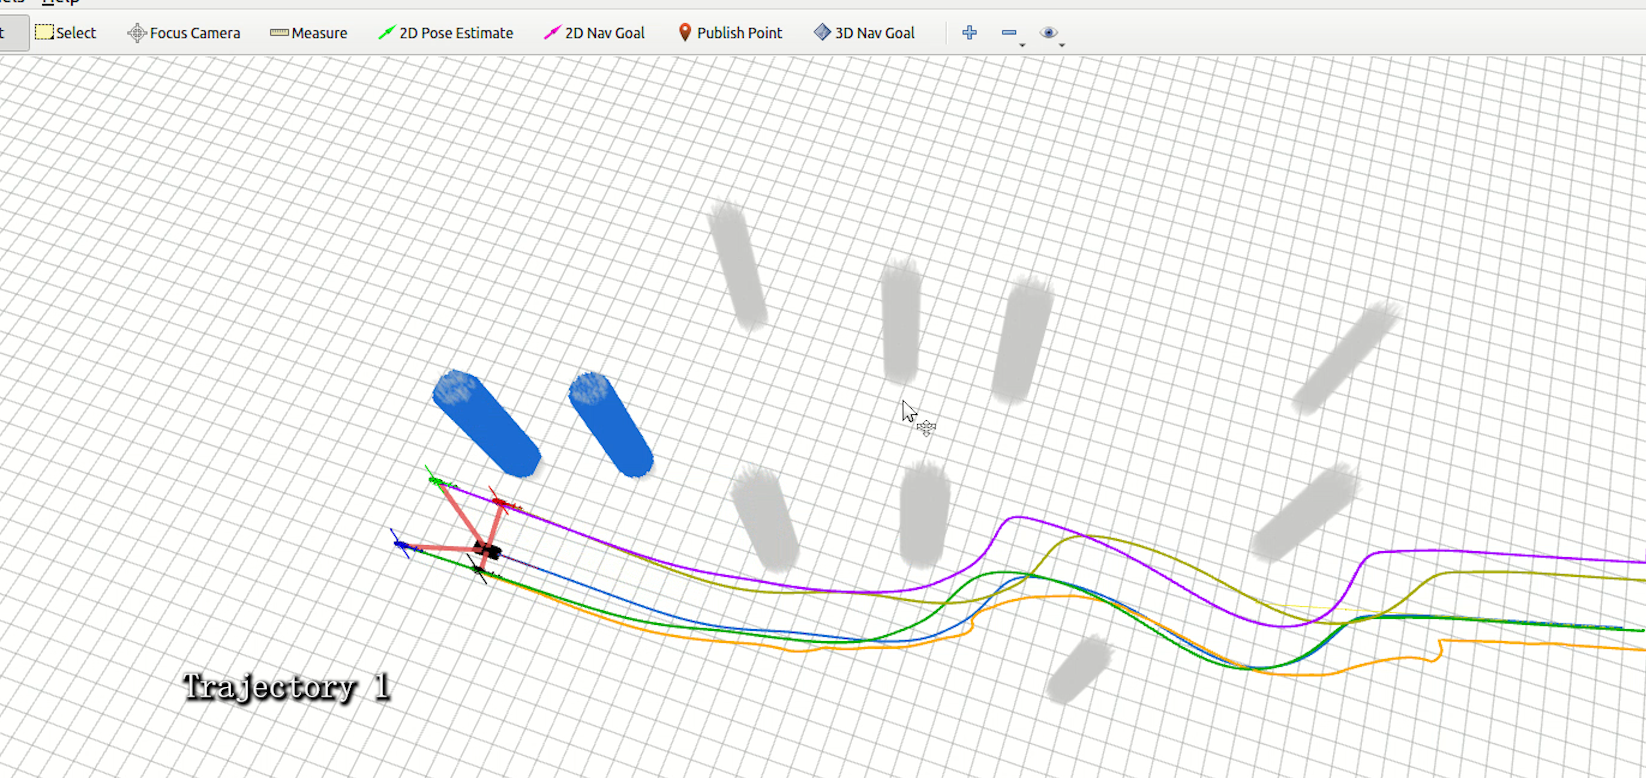
\includegraphics[width = 0.45\textwidth]{fig/figure_chap6/point_trajectory/1.png}}\quad
    \subfloat[轨迹2]{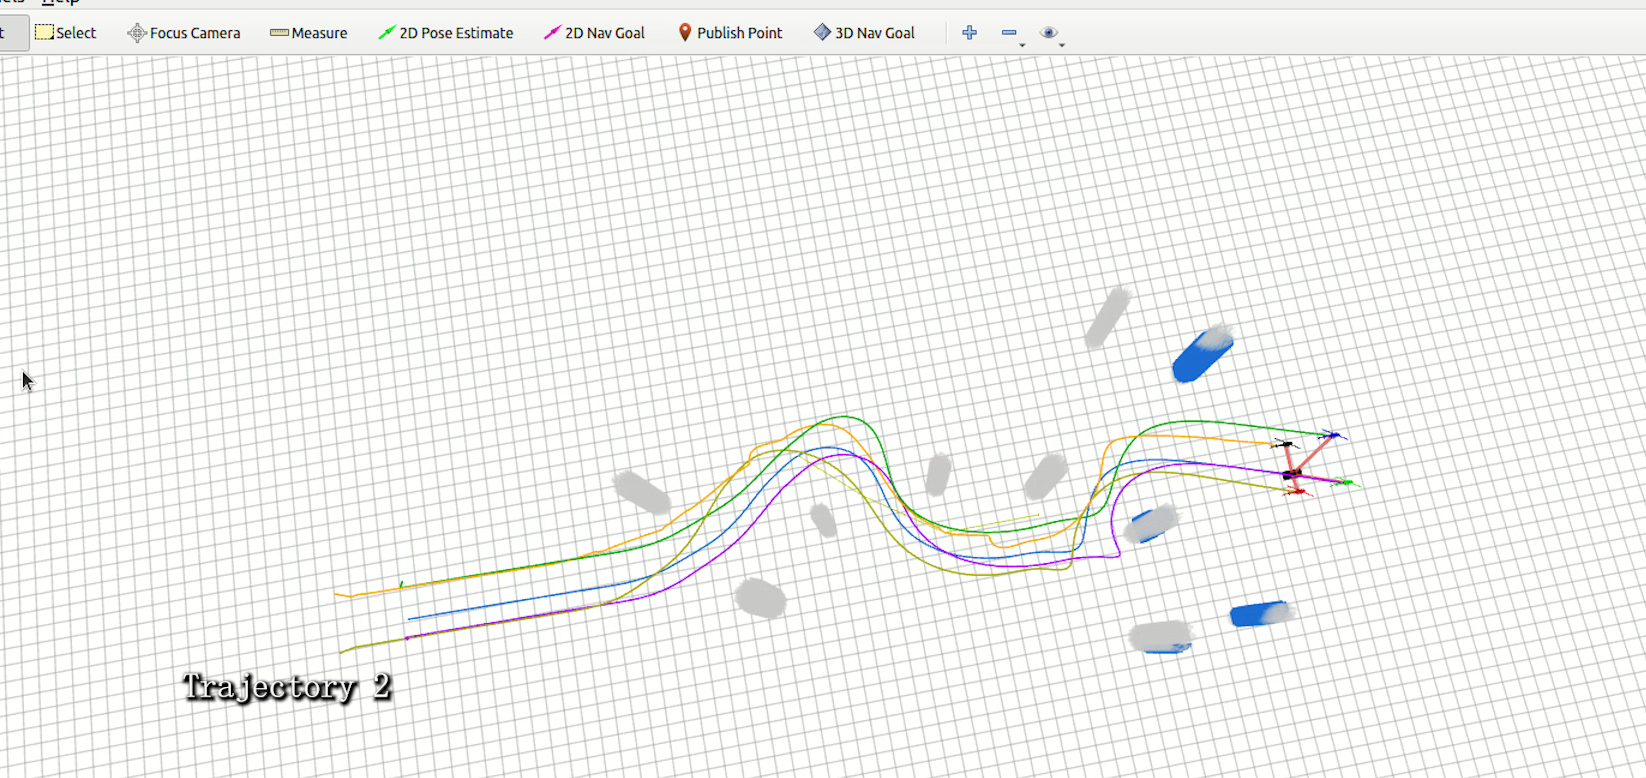
\includegraphics[width = 0.45\textwidth]{fig/figure_chap6/point_trajectory/2.png}}\\
    \subfloat[轨迹3]{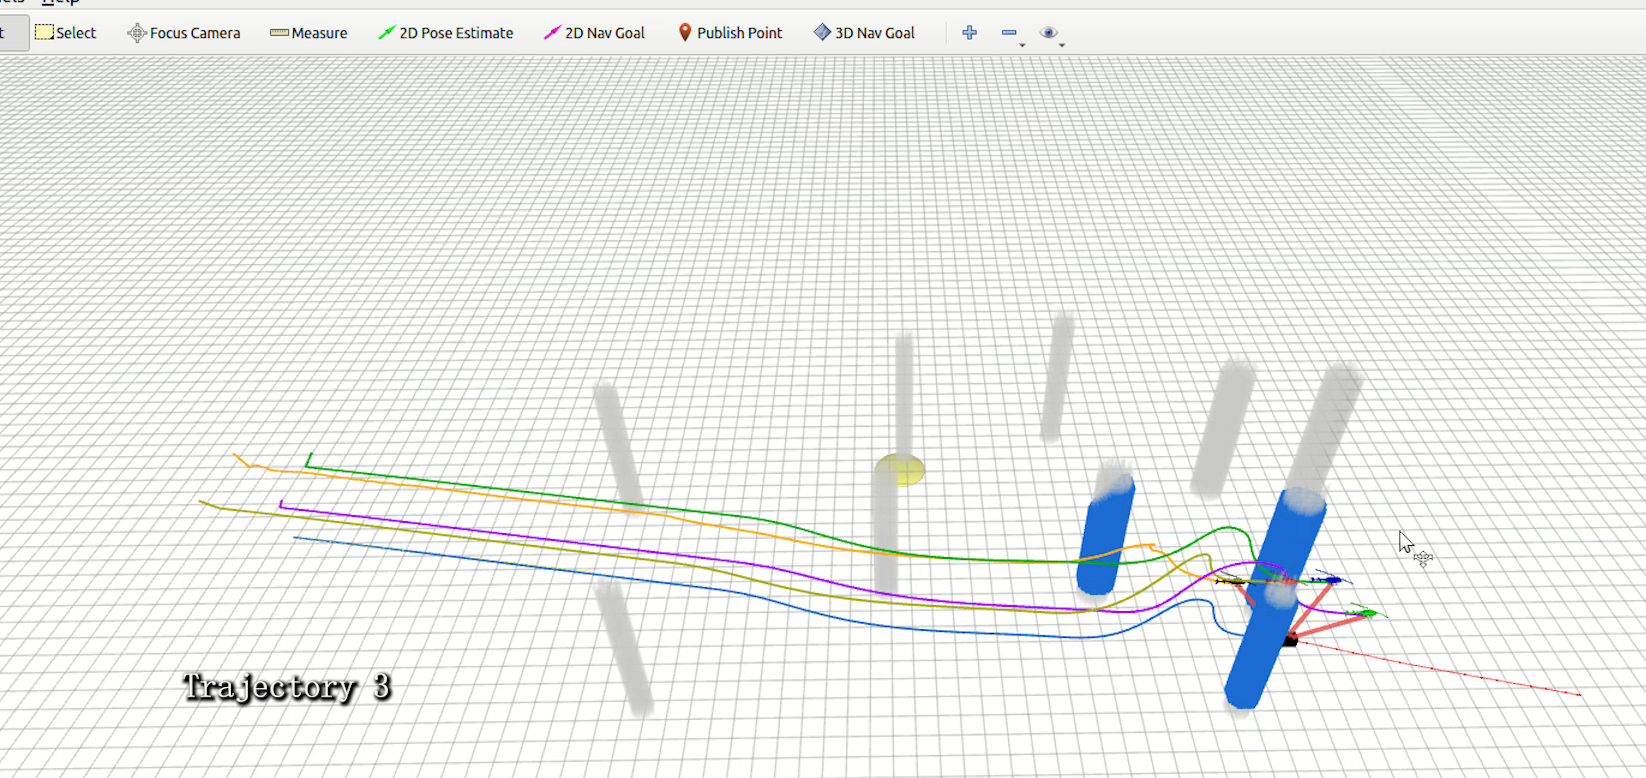
\includegraphics[width = 0.45\textwidth]{fig/figure_chap6/point_trajectory/3.png}}\quad
    \subfloat[轨迹4]{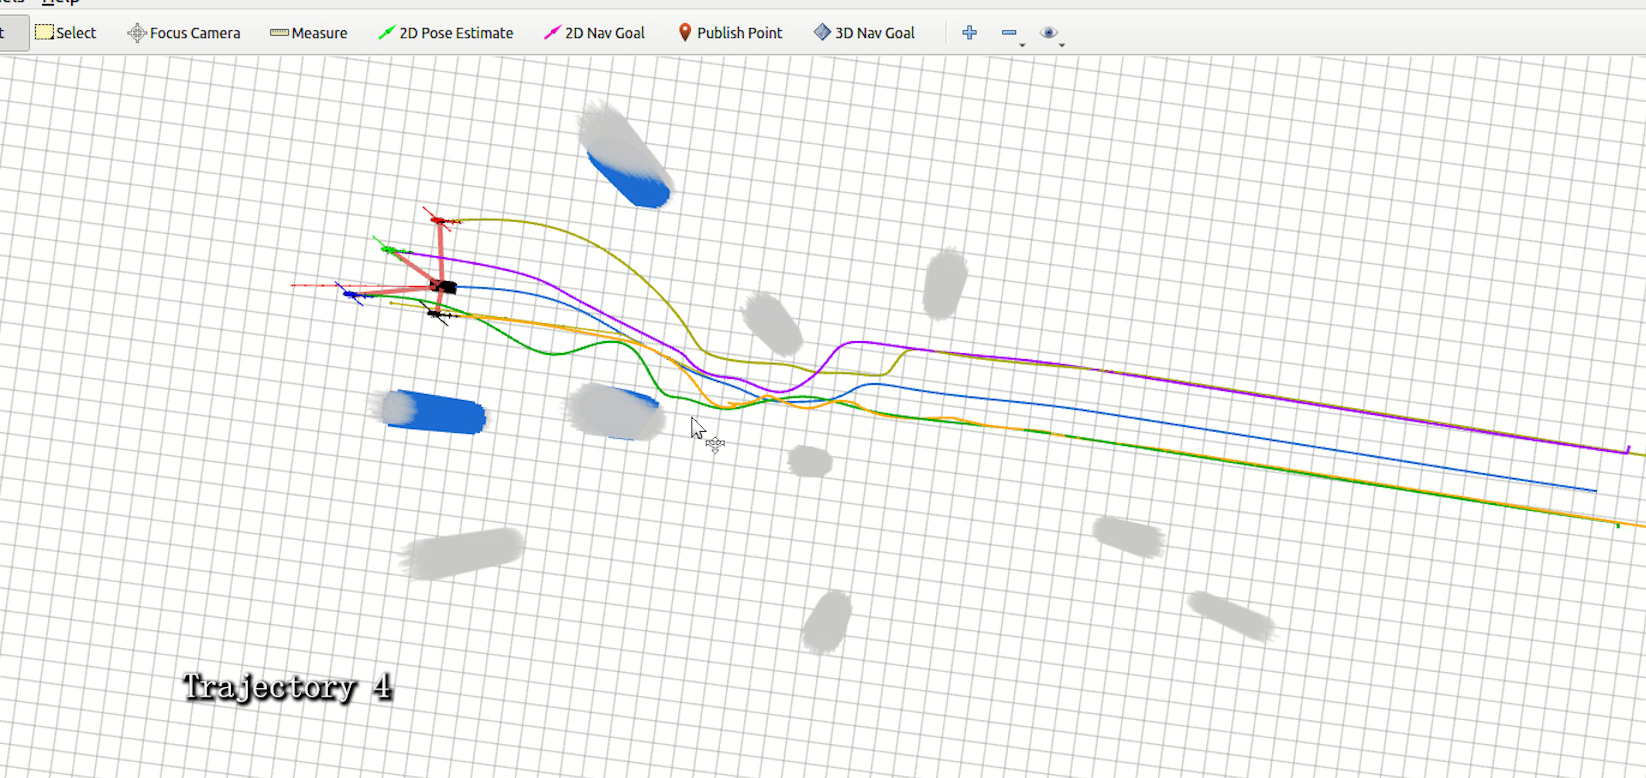
\includegraphics[width = 0.45\textwidth]{fig/figure_chap6/point_trajectory/4.png}}\\
    \subfloat[轨迹5]{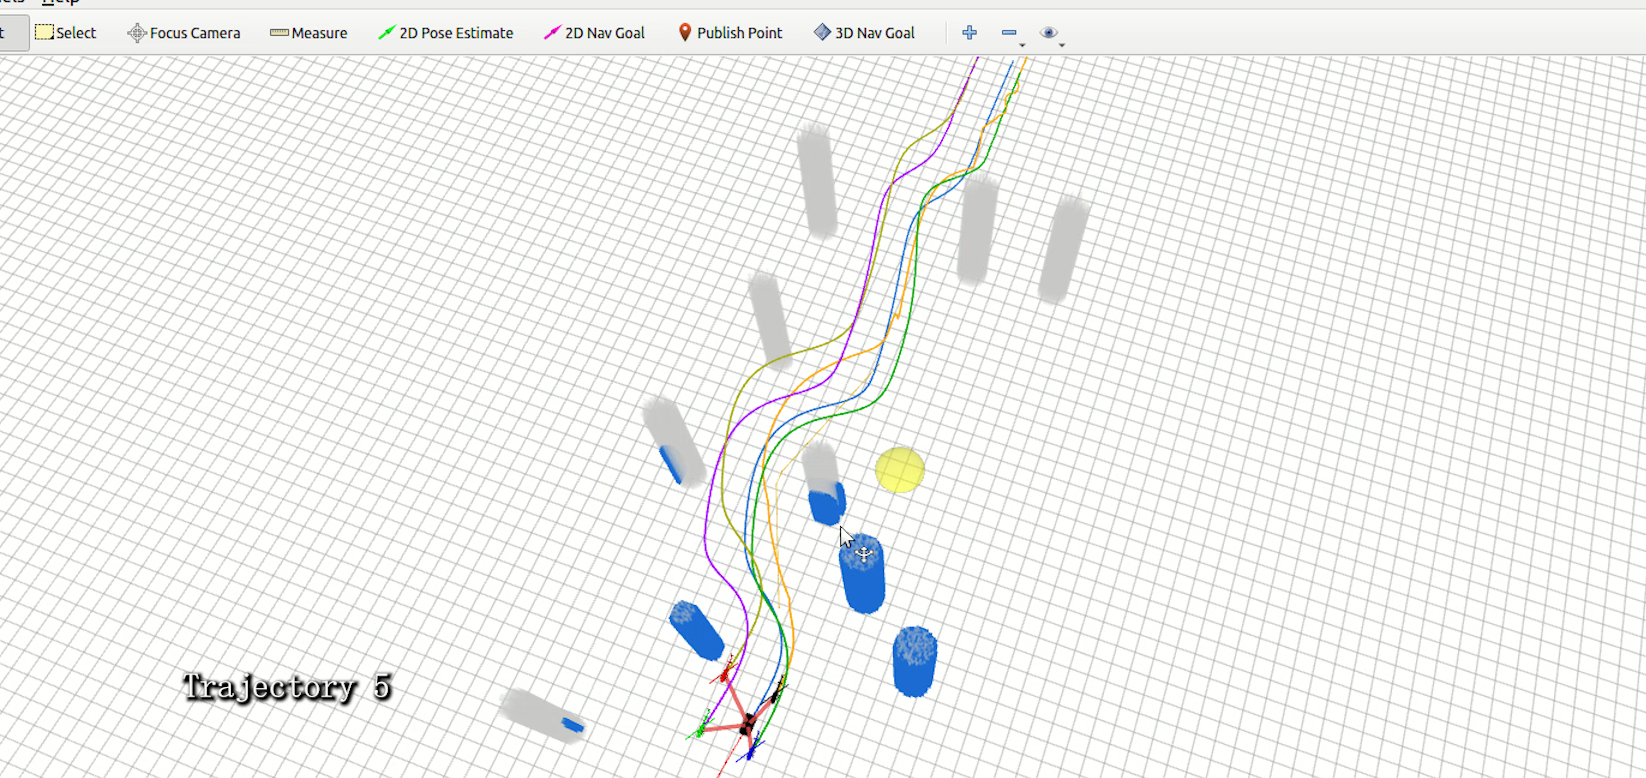
\includegraphics[width = 0.45\textwidth]{fig/figure_chap6/point_trajectory/5.png}}\quad
    \subfloat[轨迹6]{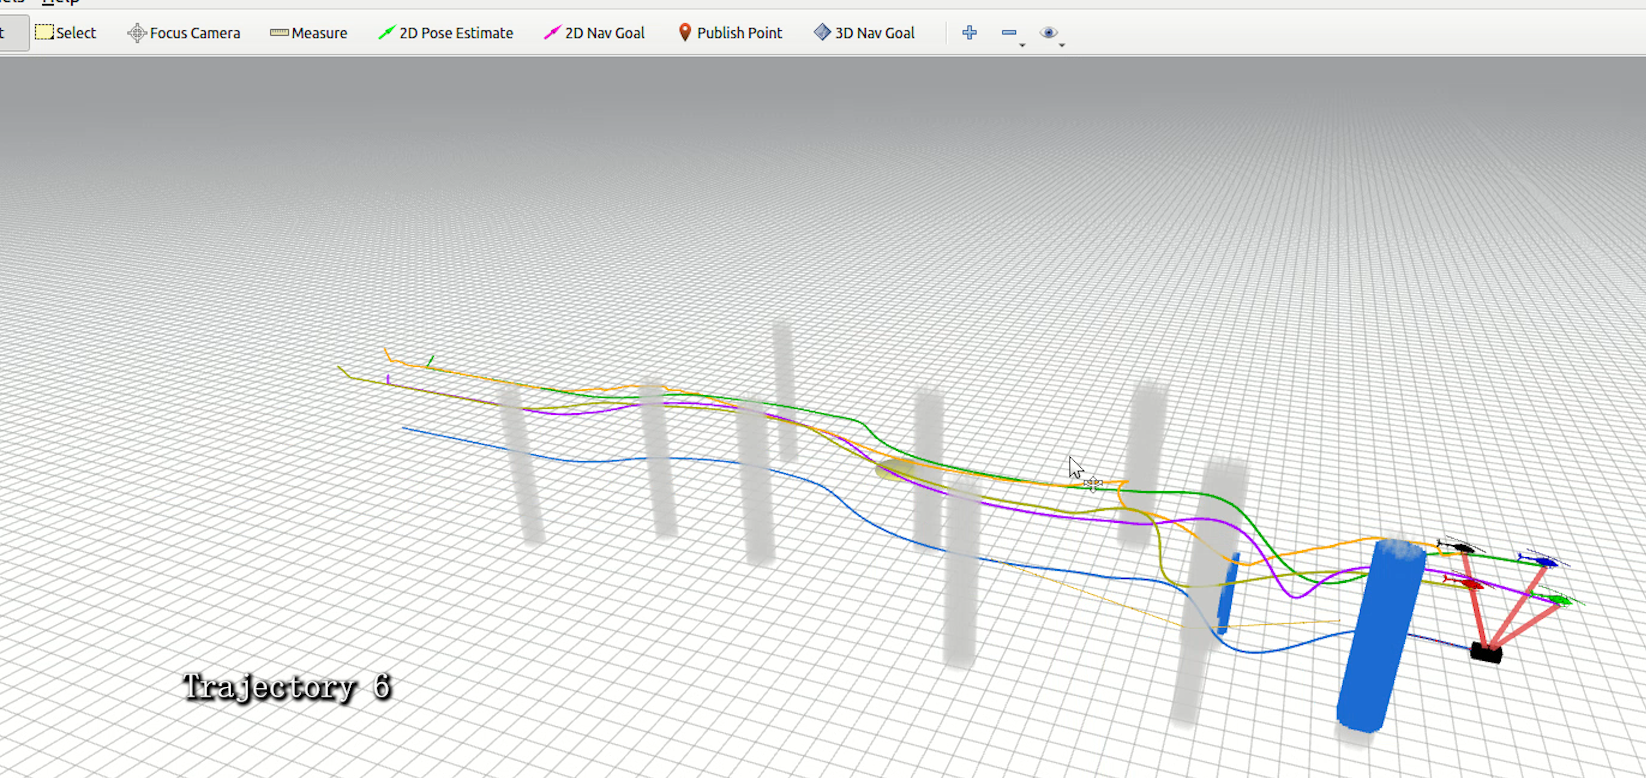
\includegraphics[width = 0.45\textwidth]{fig/figure_chap6/point_trajectory/6.png}}\\
    \subfloat[轨迹7]{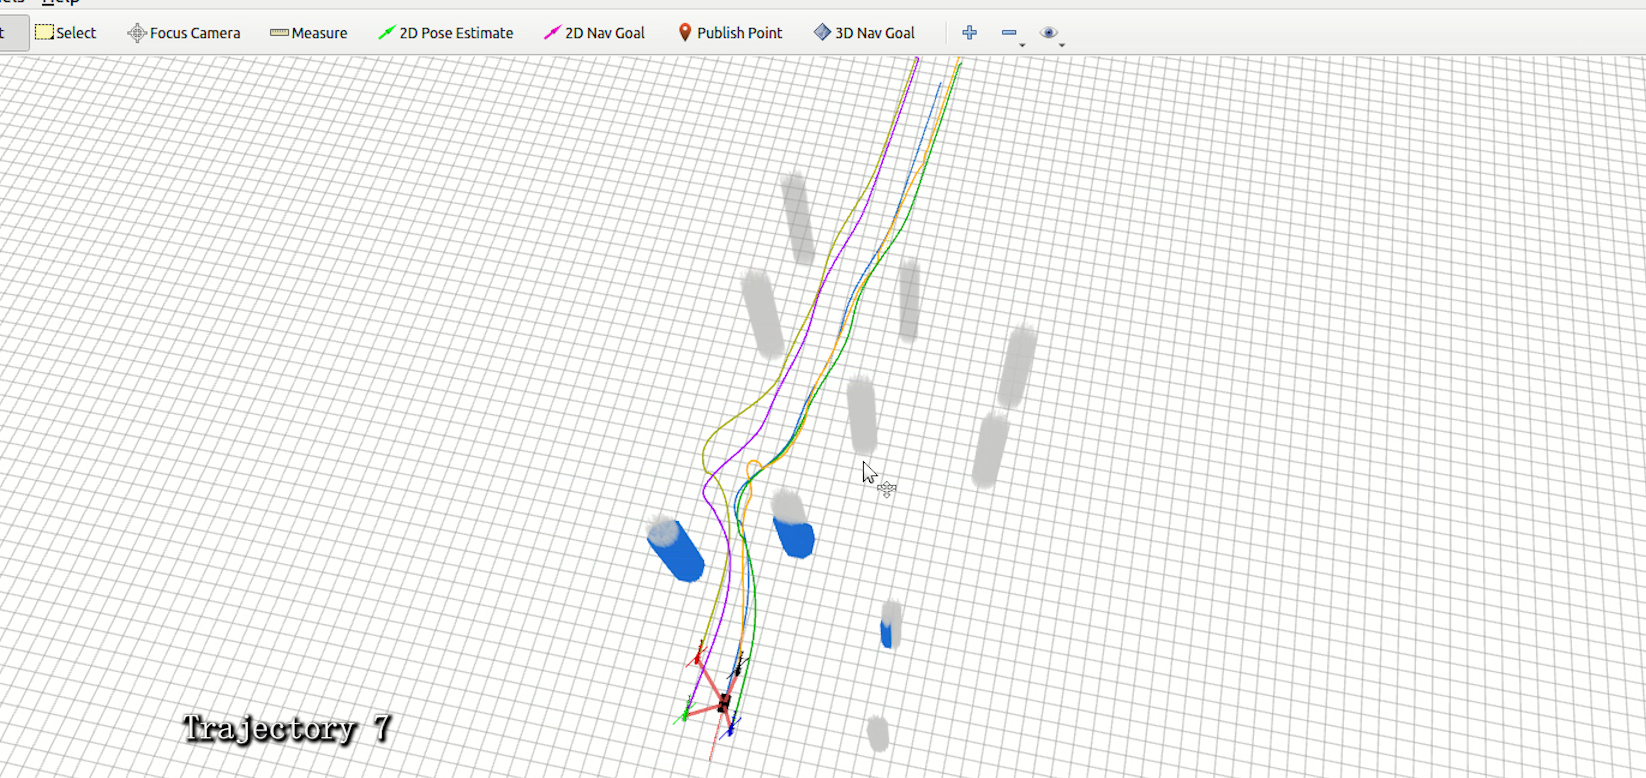
\includegraphics[width = 0.45\textwidth]{fig/figure_chap6/point_trajectory/7.png}}\quad
    \subfloat[轨迹8]{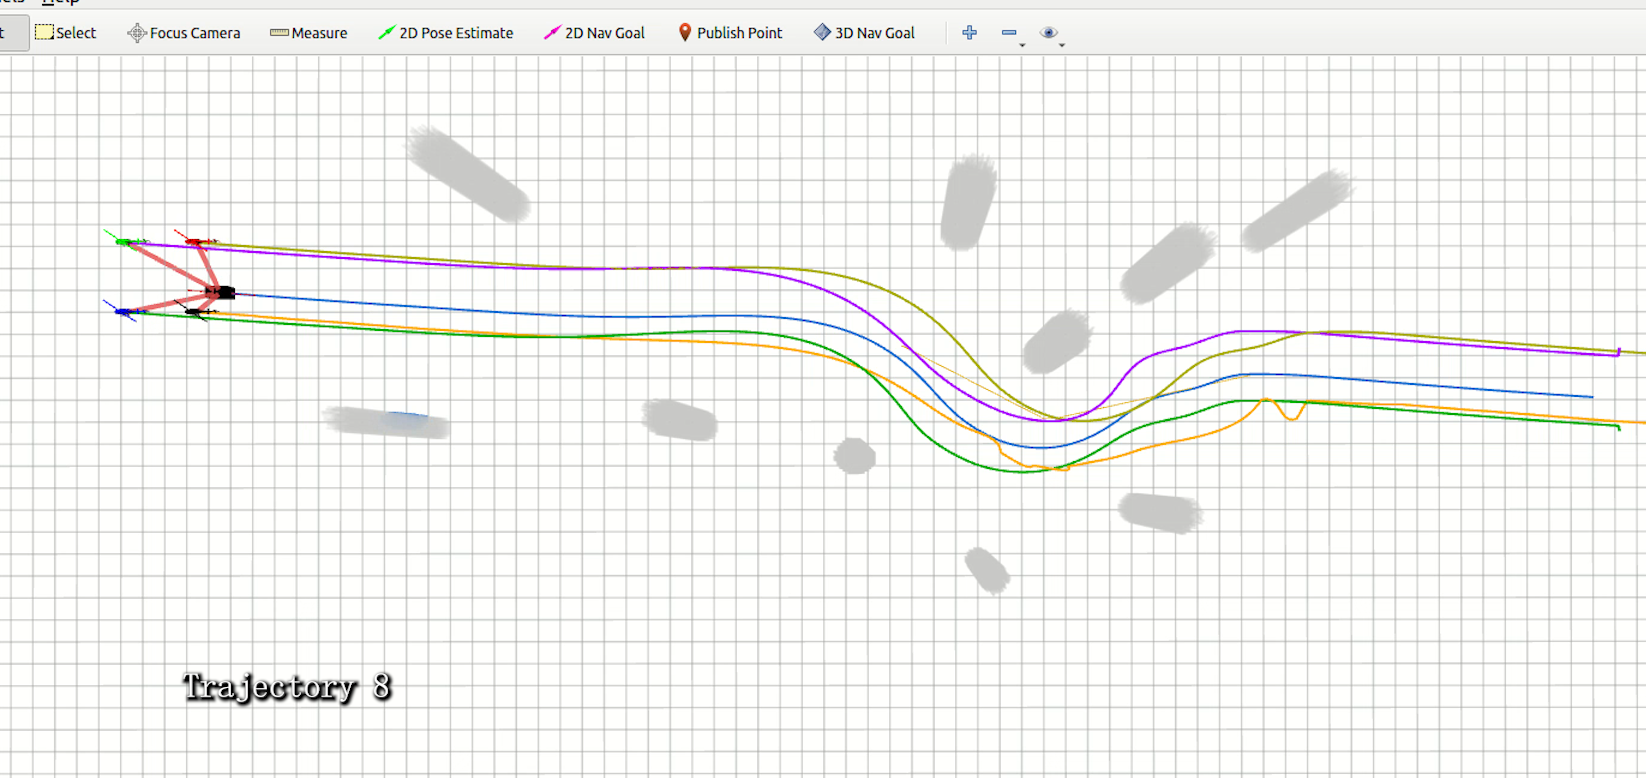
\includegraphics[width = 0.45\textwidth]{fig/figure_chap6/point_trajectory/8.png}}\\
    \caption{质点吊挂物协同吊挂系统避障轨迹\label{point_trajectory}}
\end{figure}

图\ref{point_trajectory}给出了吊挂物建模为质点时的四直升机协同吊挂系统避障仿真结果。可以看出,随机生成8次地图,基于本文提出的避障优化算法,协同吊挂系统均具备避障能力。更为详细的仿真过程见视频链接\href{https://www.bilibili.com/video/BV1EA411Z7AQ/}{https://www.bilibili.com/video/BV1EA411Z7AQ/}。由视频可见,8次仿真过程中,吊挂物、直升机、吊索距离障碍物都有一定距离,直升机间无碰撞,吊索间无交叉,体现了本文提出了基于微分平坦和minco的避障策略的有效性。同时发现,虽然吊挂物建模为质点时$\lambda_{\rm{T}}$较小,相比直升机2、3、4,直升机1的机动性依然更大,这与微分平坦输出的选择有关,详细分析见上文。

从上述8条轨迹优化过程中随机选取3次迭代,详细给出了各惩罚函数随迭代步数的变化,见图\ref{point_cost}。考虑到前20步惩罚函数的数量级一般较大,为了更好地展示各惩罚函数的收敛过程,图中迭代步数即横坐标从20开始。从图中可以看出,迭代20步后,最小能量惩罚项$J_{\rm{e}}\lambda_{\rm{e}}$、总时间惩罚项$J_{\rm{T}}\lambda_{\rm{T}}$、控制点均匀分布惩罚项$J_{\rm{e}}\lambda_{\rm{e}}$的值较小且在不断收敛,吊挂物避障惩罚项$J_{\rm{o,L}}\lambda_{\rm{o,L}}$、吊挂物状态量可行性惩罚项$J_{\rm{f,L}}\lambda_{\rm{f,L}}$、吊索避障惩罚项$J_{\rm{o,C}}\lambda_{\rm{o,C}}$、吊索力可行性惩罚项$J_{\rm{f,C}}\lambda_{\rm{f,C}}$为0且不变,直升机避障惩罚项$J_{\rm{o,H}}\lambda_{\rm{o,H}}$、直升机间避免相互碰撞惩罚项$J_{\rm{o,d}}\lambda_{\rm{o,d}}$虽然一开始有波动但80步后均收敛到较小值。总惩罚项$K$为上述各惩罚项的和,80步后均收敛到较小值。可见,惩罚项随迭代步数是收敛的,反映了避障优化算法的可行性。

对应图\ref{point_trajectory}中的8条避障轨迹,图\ref{point_time}给出了每条轨迹每次迭代消耗的时间。可见,除少数迭代消耗时间较大外,其余94.36\%迭代消耗时间均小于100 ms即0.1 s,8条轨迹共390次迭代平均优化时间为29.56 ms,体现了所提优化算法的实时性。需要说明的是,本文仿真是在虚拟机中进行的,运行速度受限。若提升硬件性能,计算速度应该会更快。

\begin{figure}[htb!]
    \centering
    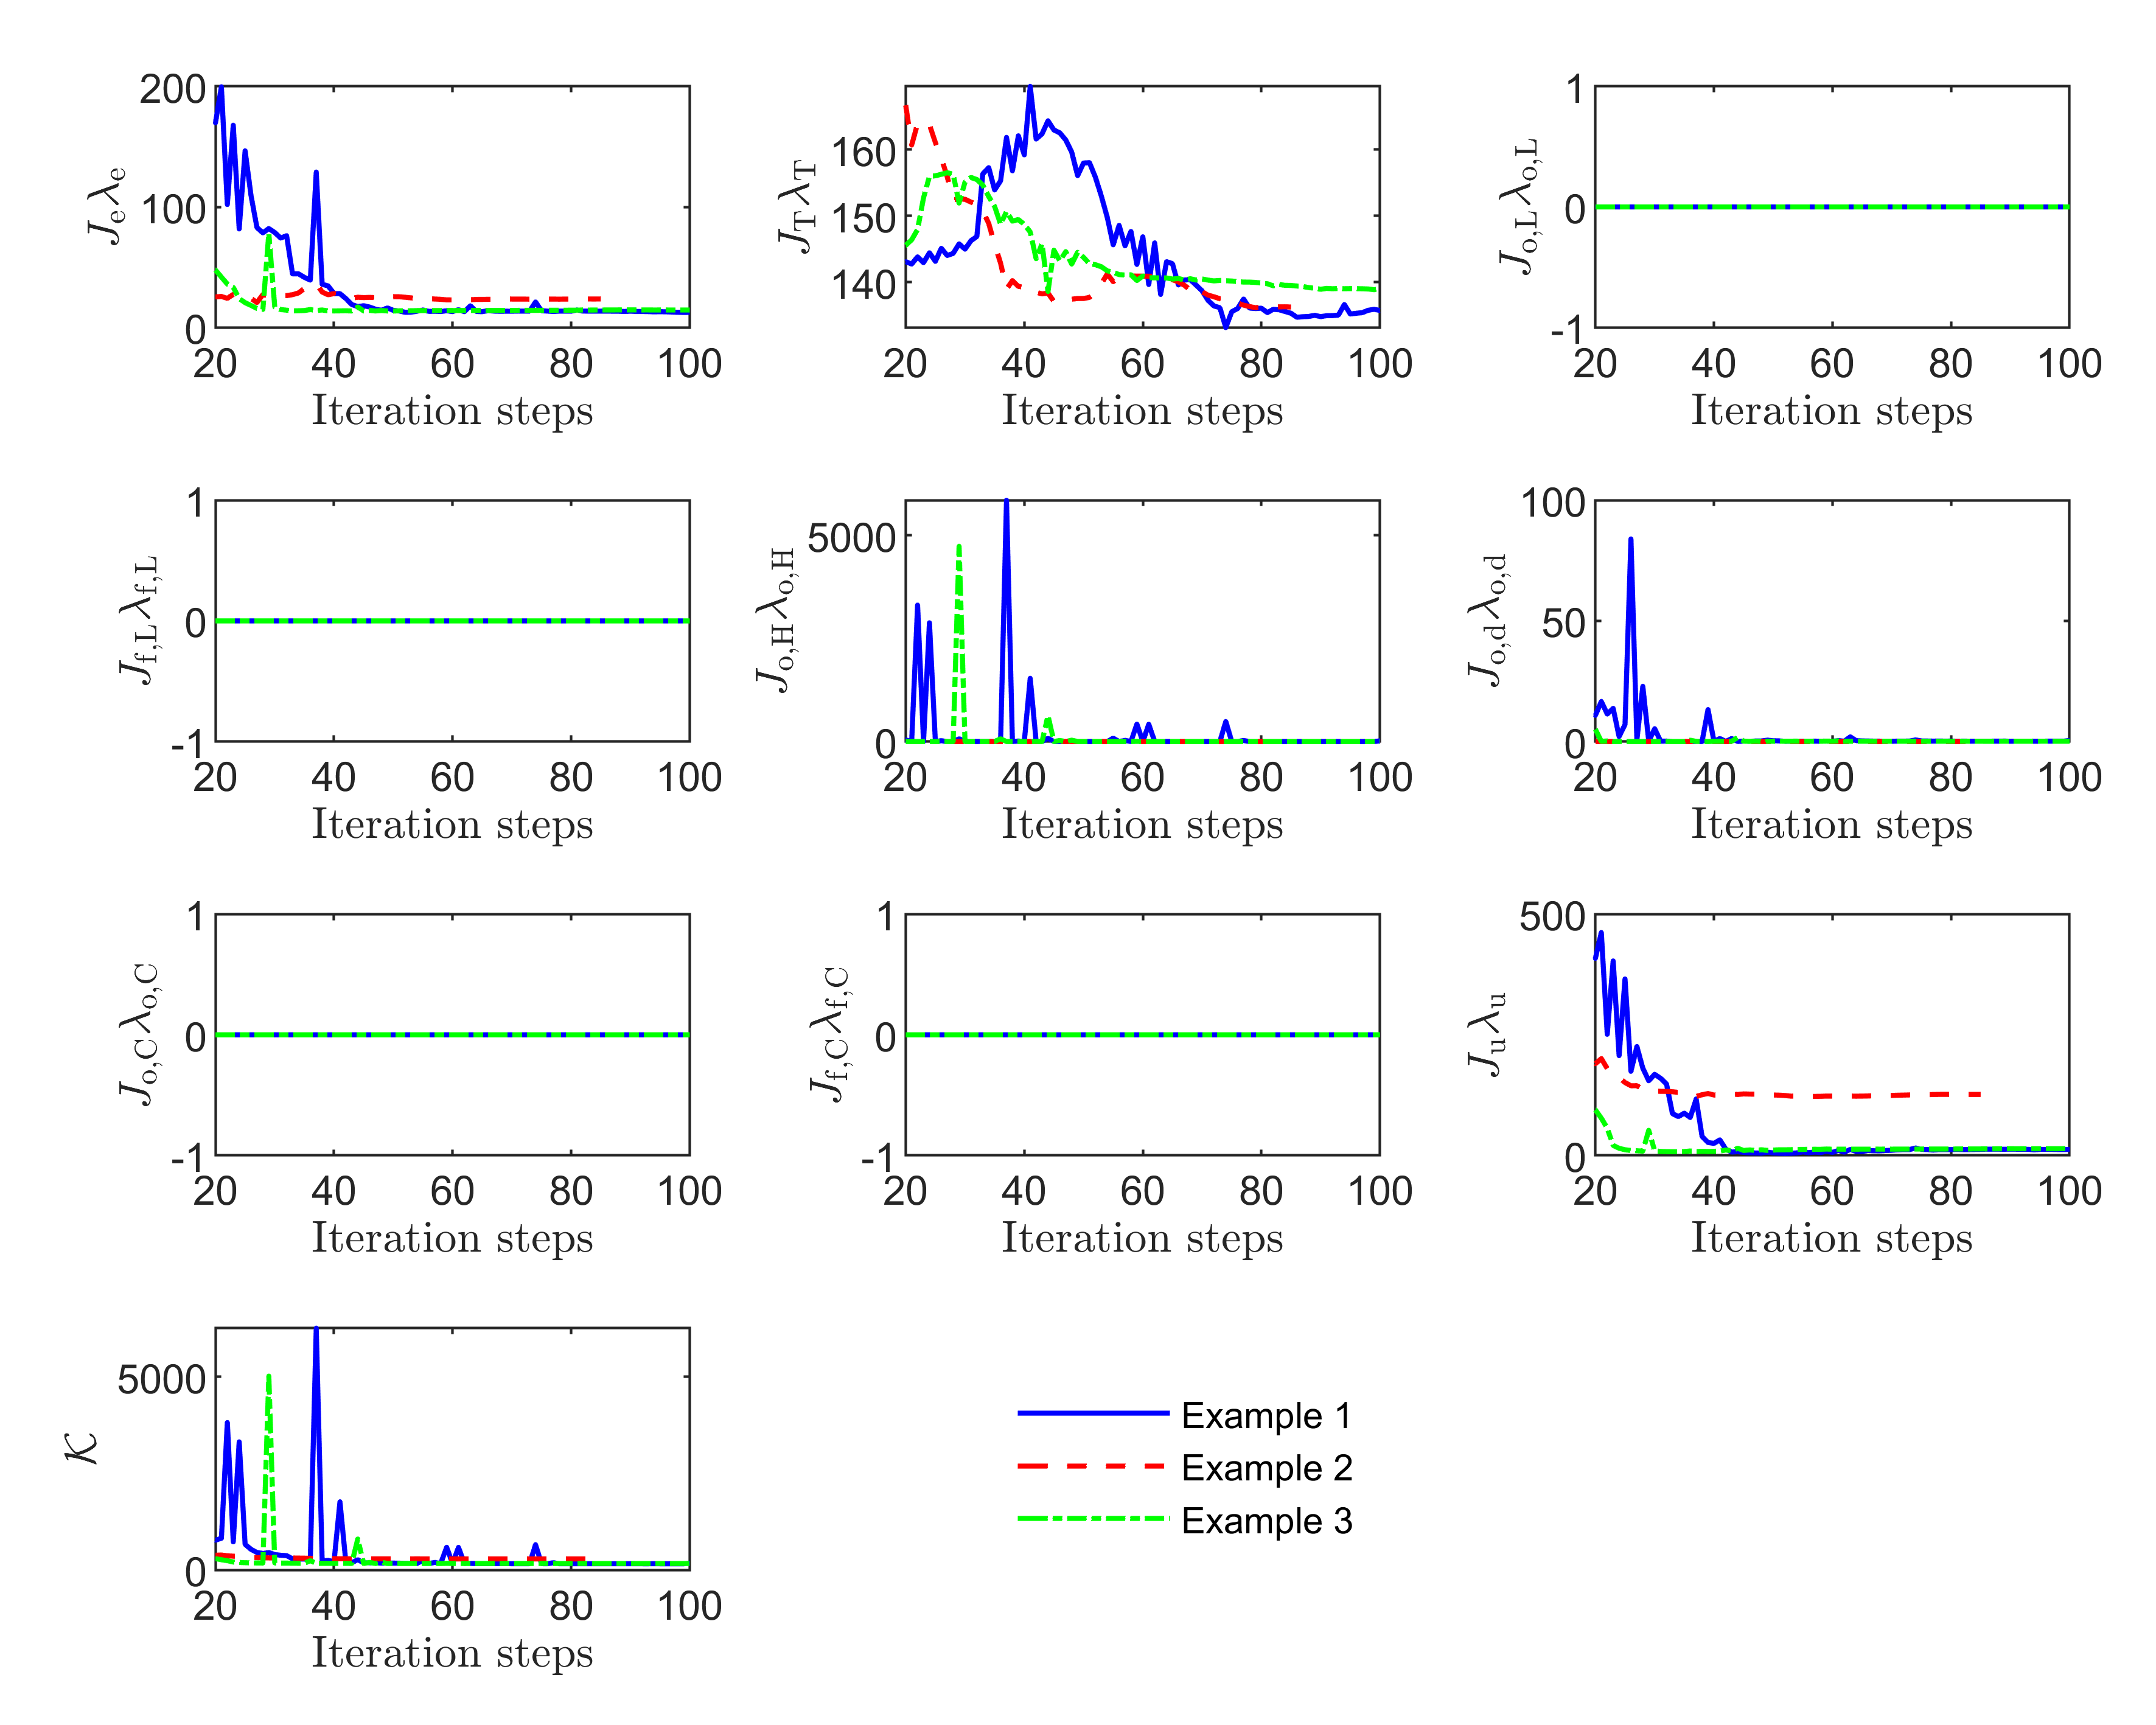
\includegraphics[width = 0.95\textwidth]{fig/figure_chap6/cost_point.png}
    \caption{刚体吊挂物协同吊挂系统代价函数随迭代步数的变化\label{point_cost}}
\end{figure}

\begin{figure}[htb!]
    \centering
    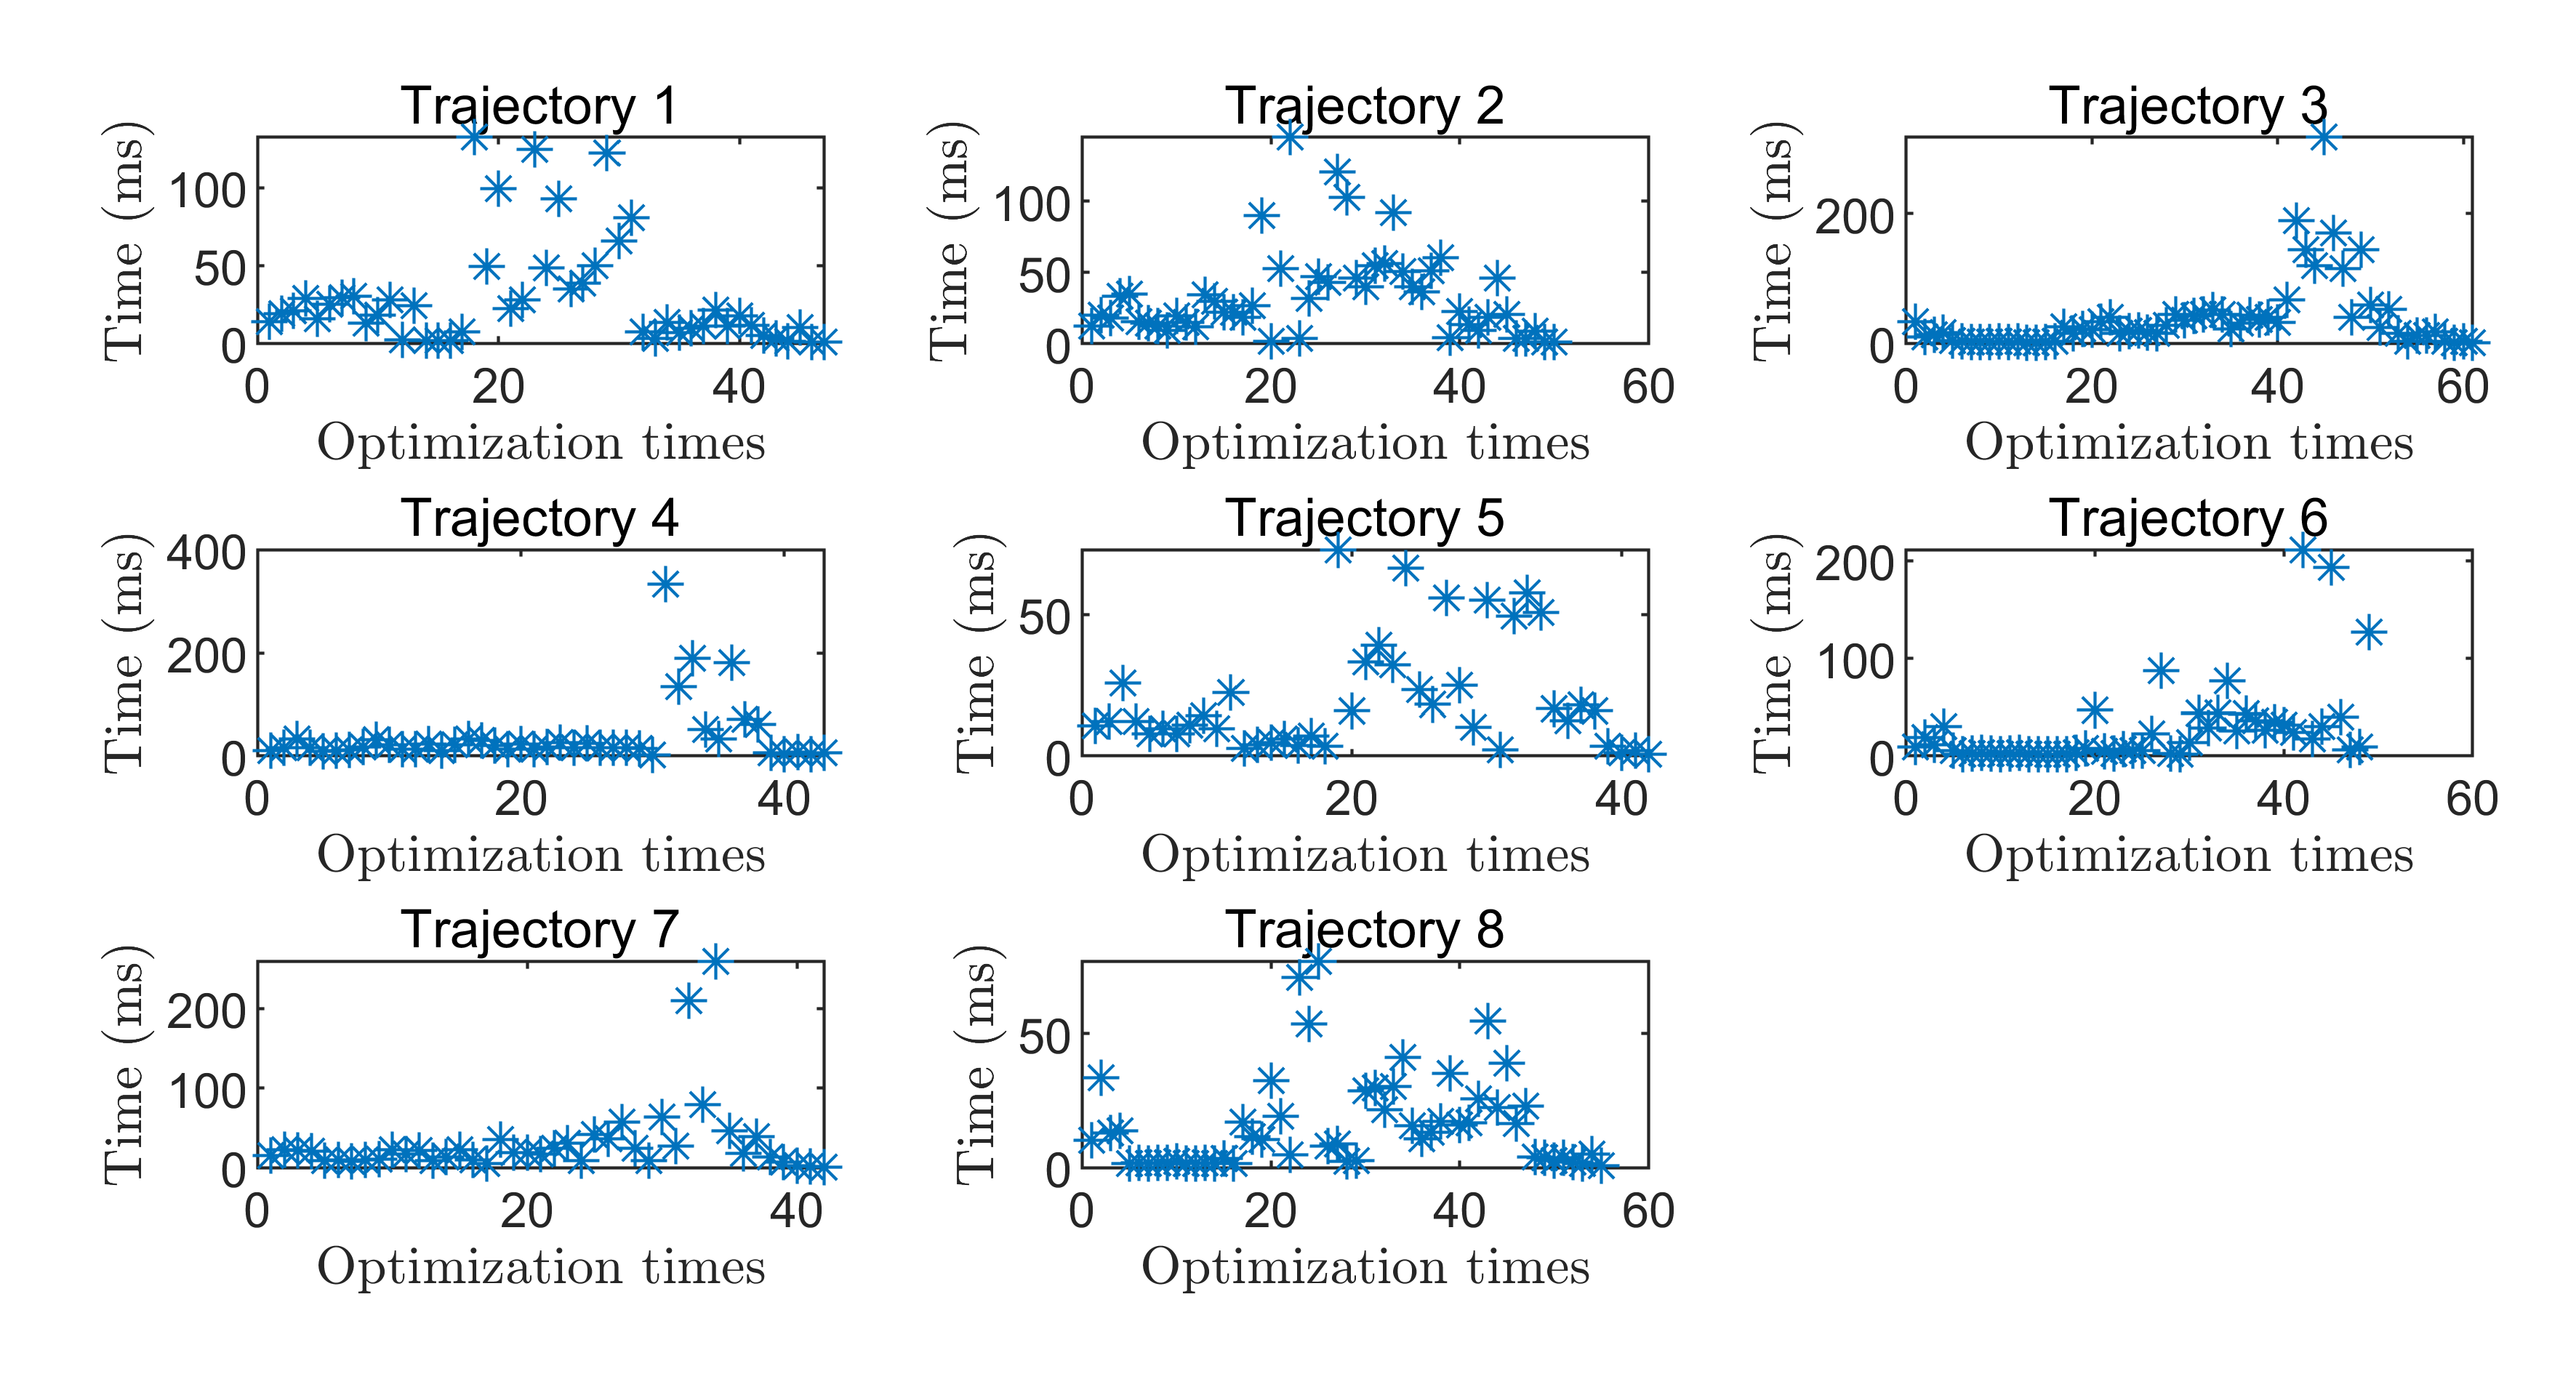
\includegraphics[width = 0.95\textwidth]{fig/figure_chap6/time_point.png}
    \caption{刚体吊挂物协同吊挂系统迭代收敛时间\label{point_time}}
\end{figure}

\subsection{刚体吊挂物仿真结果}

\begin{figure}[htb!]
    \subfloat[轨迹1]{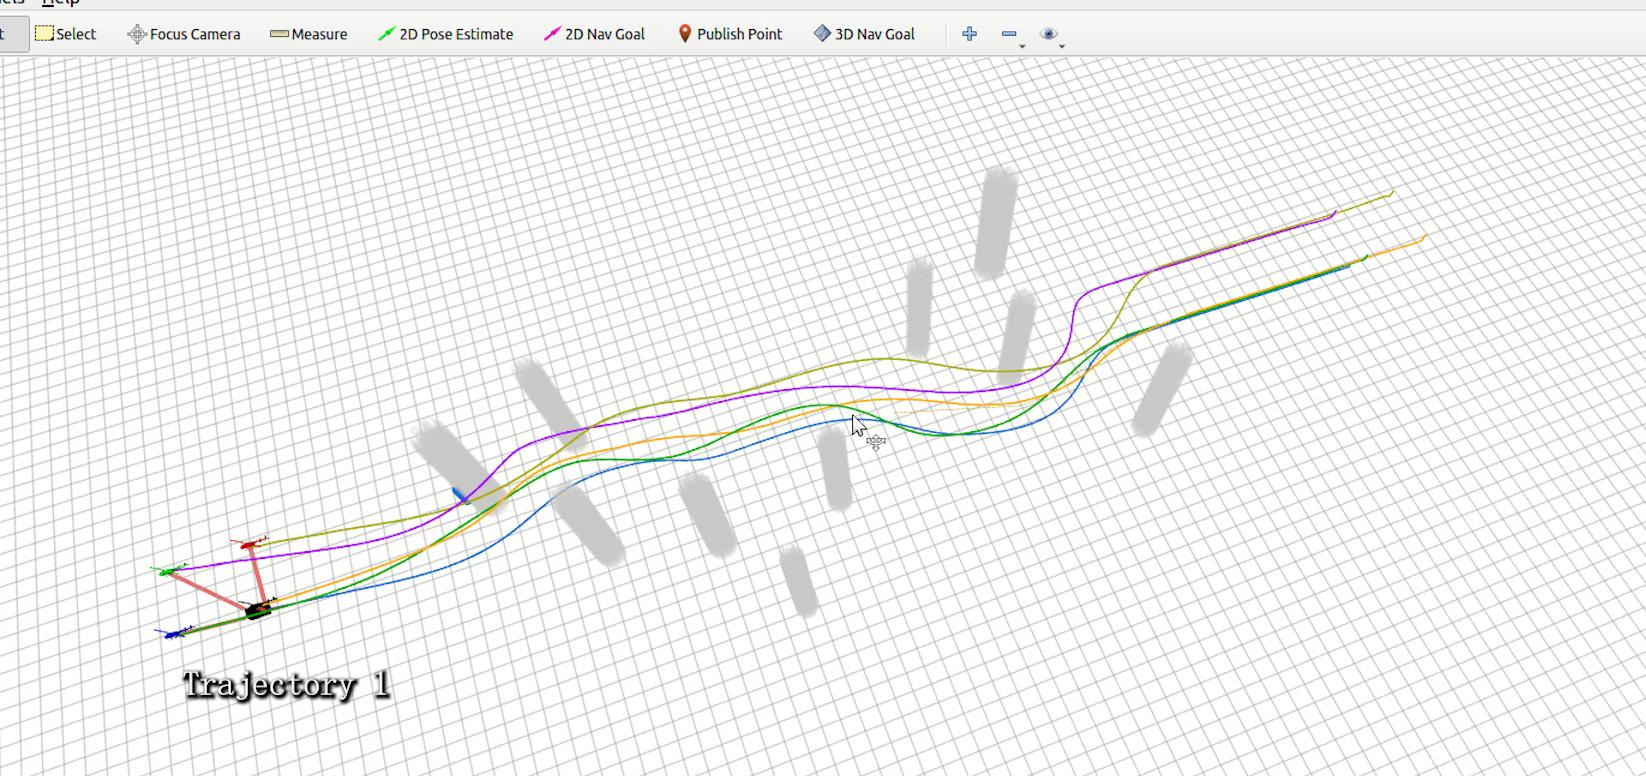
\includegraphics[width = 0.45\textwidth]{fig/figure_chap6/rigid_trajectory/1.png}}\quad
    \subfloat[轨迹2]{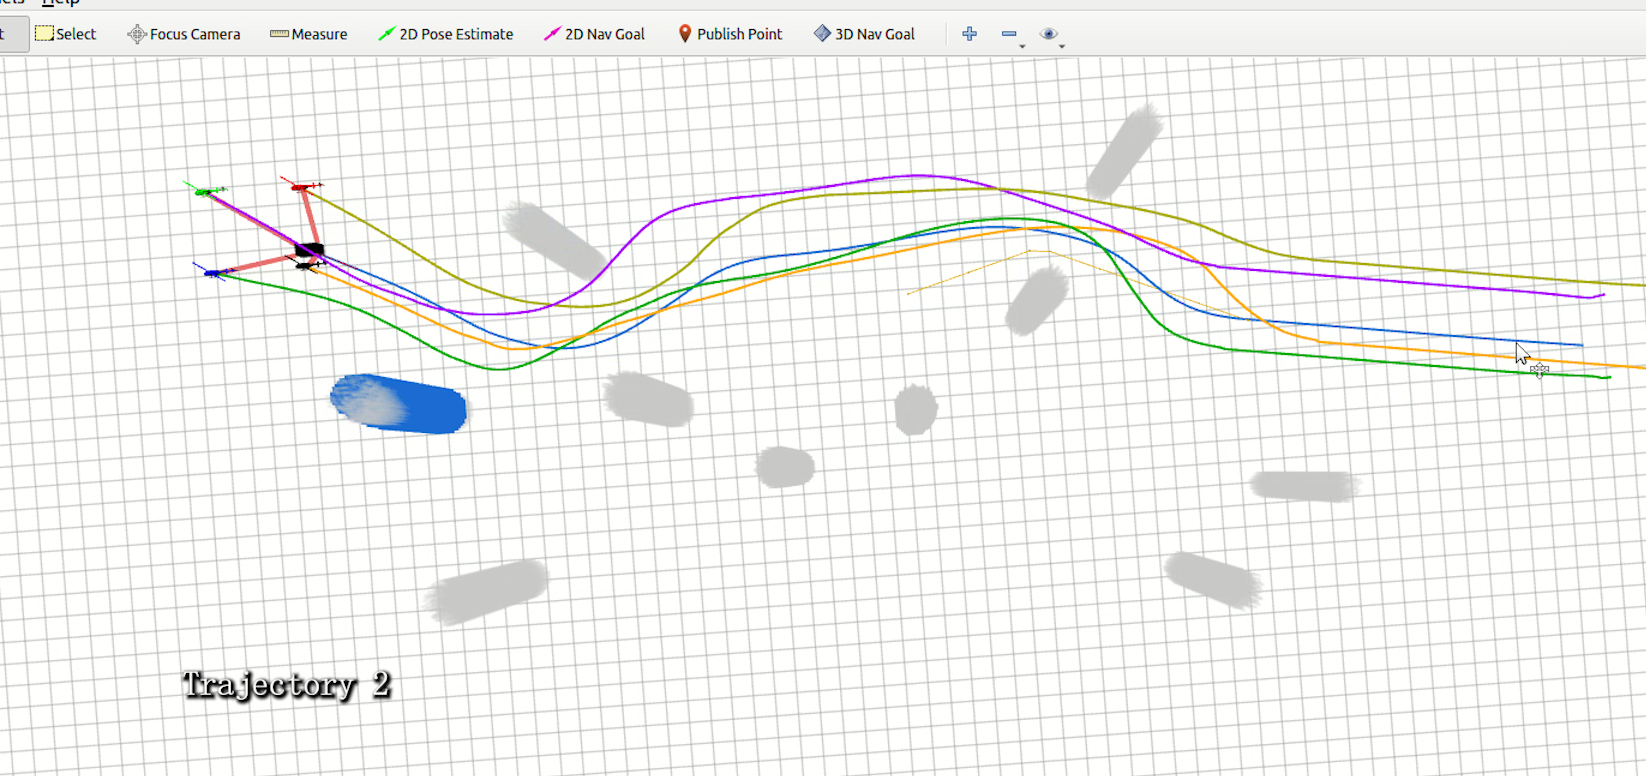
\includegraphics[width = 0.45\textwidth]{fig/figure_chap6/rigid_trajectory/2.png}}\\
    \subfloat[轨迹3]{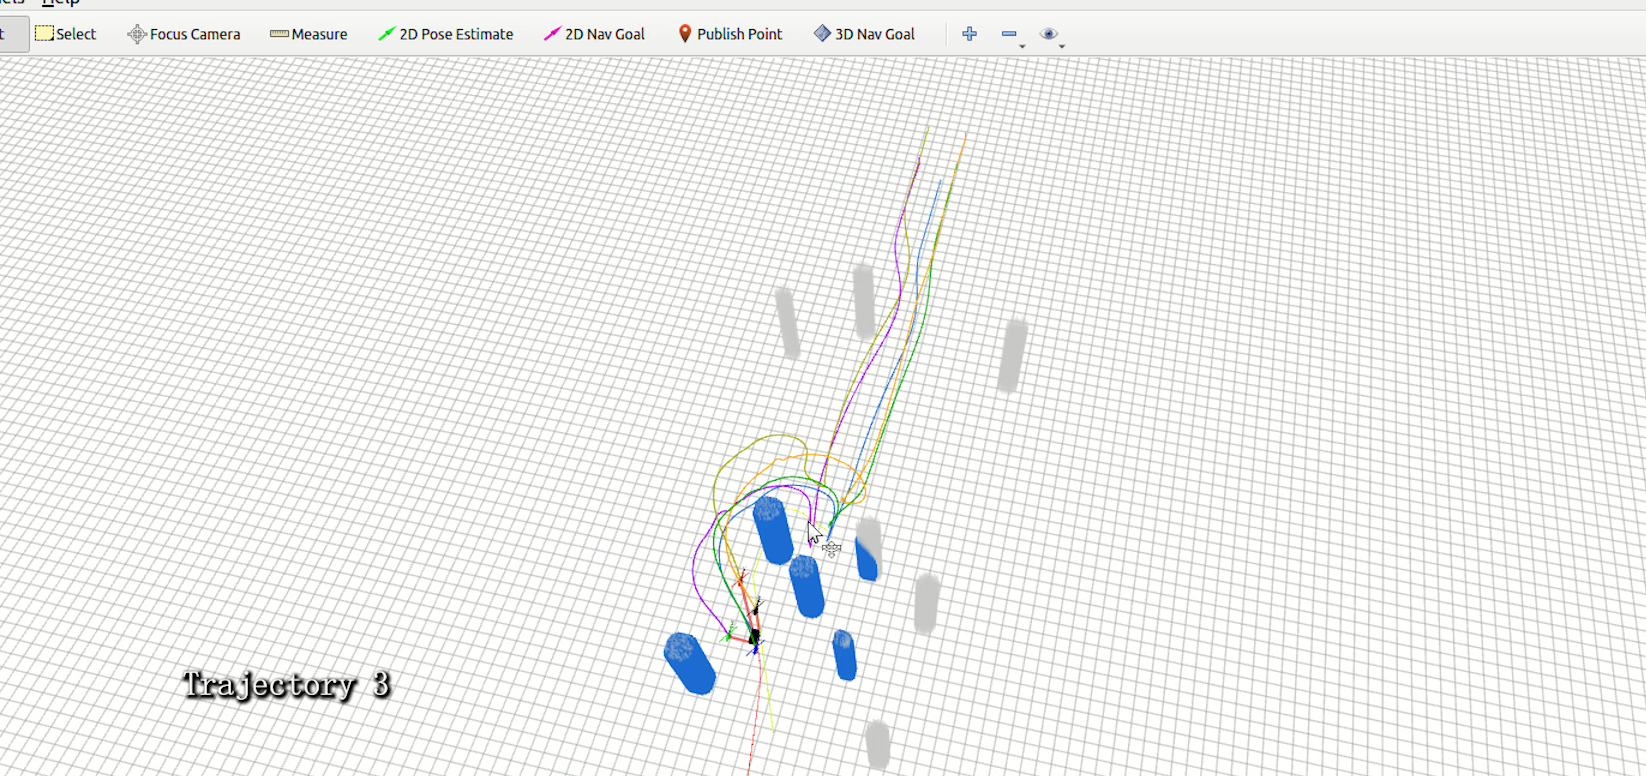
\includegraphics[width = 0.45\textwidth]{fig/figure_chap6/rigid_trajectory/3.png}}\quad
    \subfloat[轨迹4]{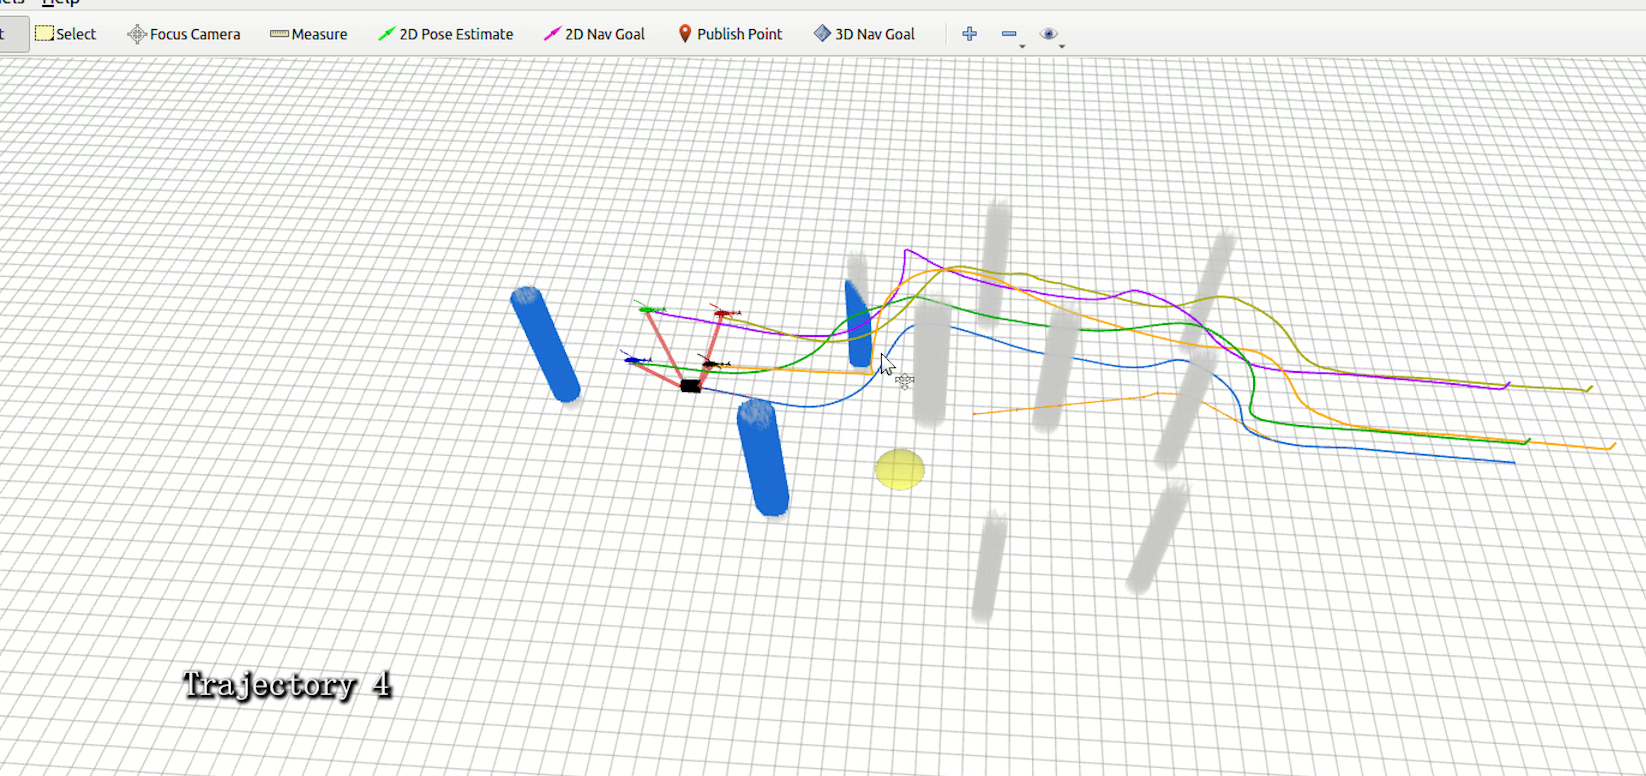
\includegraphics[width = 0.45\textwidth]{fig/figure_chap6/rigid_trajectory/4.png}}\\
    \subfloat[轨迹5]{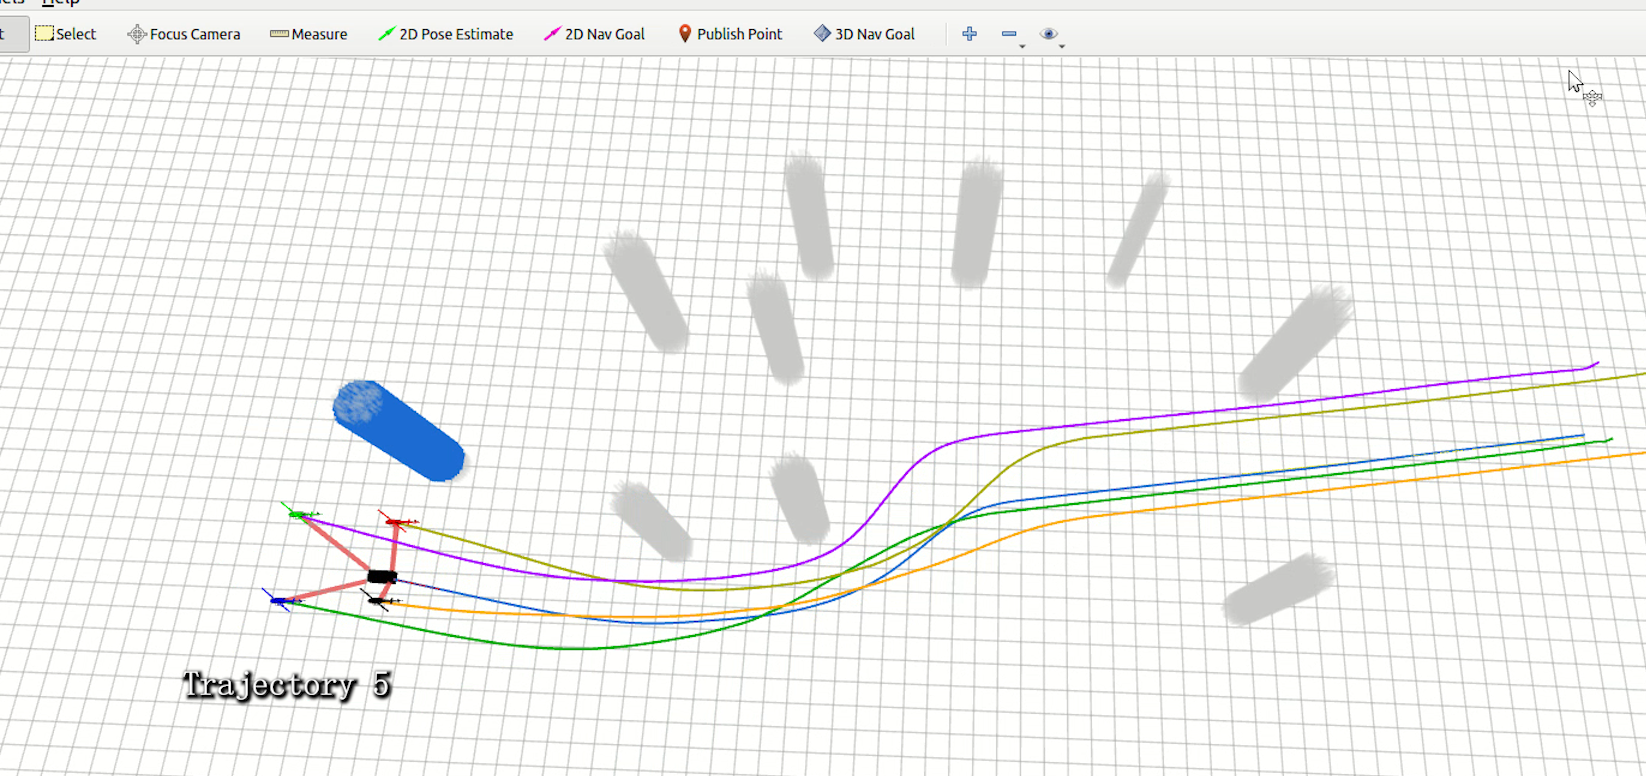
\includegraphics[width = 0.45\textwidth]{fig/figure_chap6/rigid_trajectory/5.png}}\quad
    \subfloat[轨迹6]{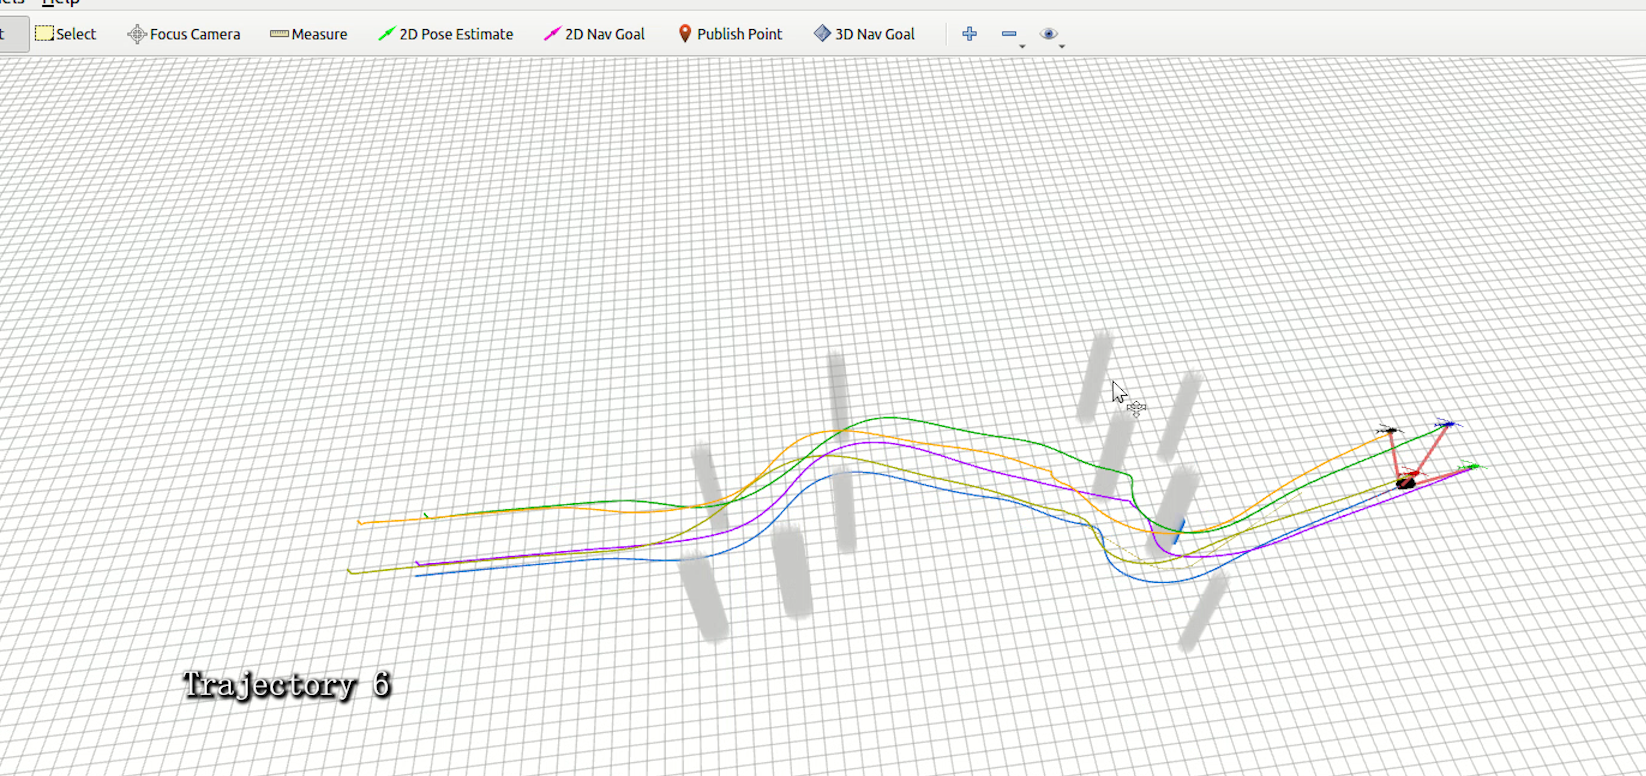
\includegraphics[width = 0.45\textwidth]{fig/figure_chap6/rigid_trajectory/6.png}}\\
    \subfloat[轨迹7]{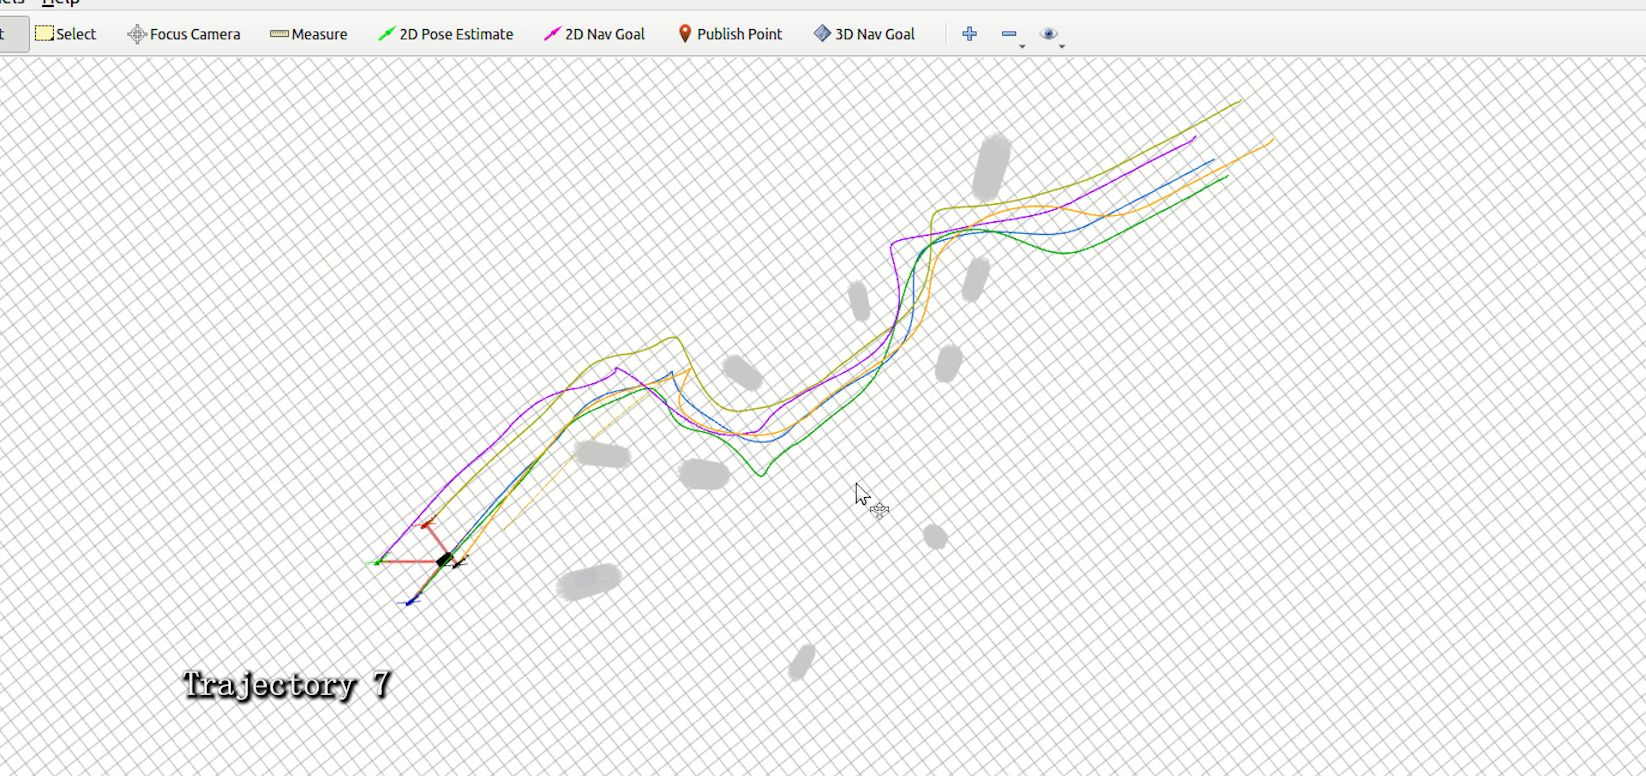
\includegraphics[width = 0.45\textwidth]{fig/figure_chap6/rigid_trajectory/7.png}}\quad
    \subfloat[轨迹8]{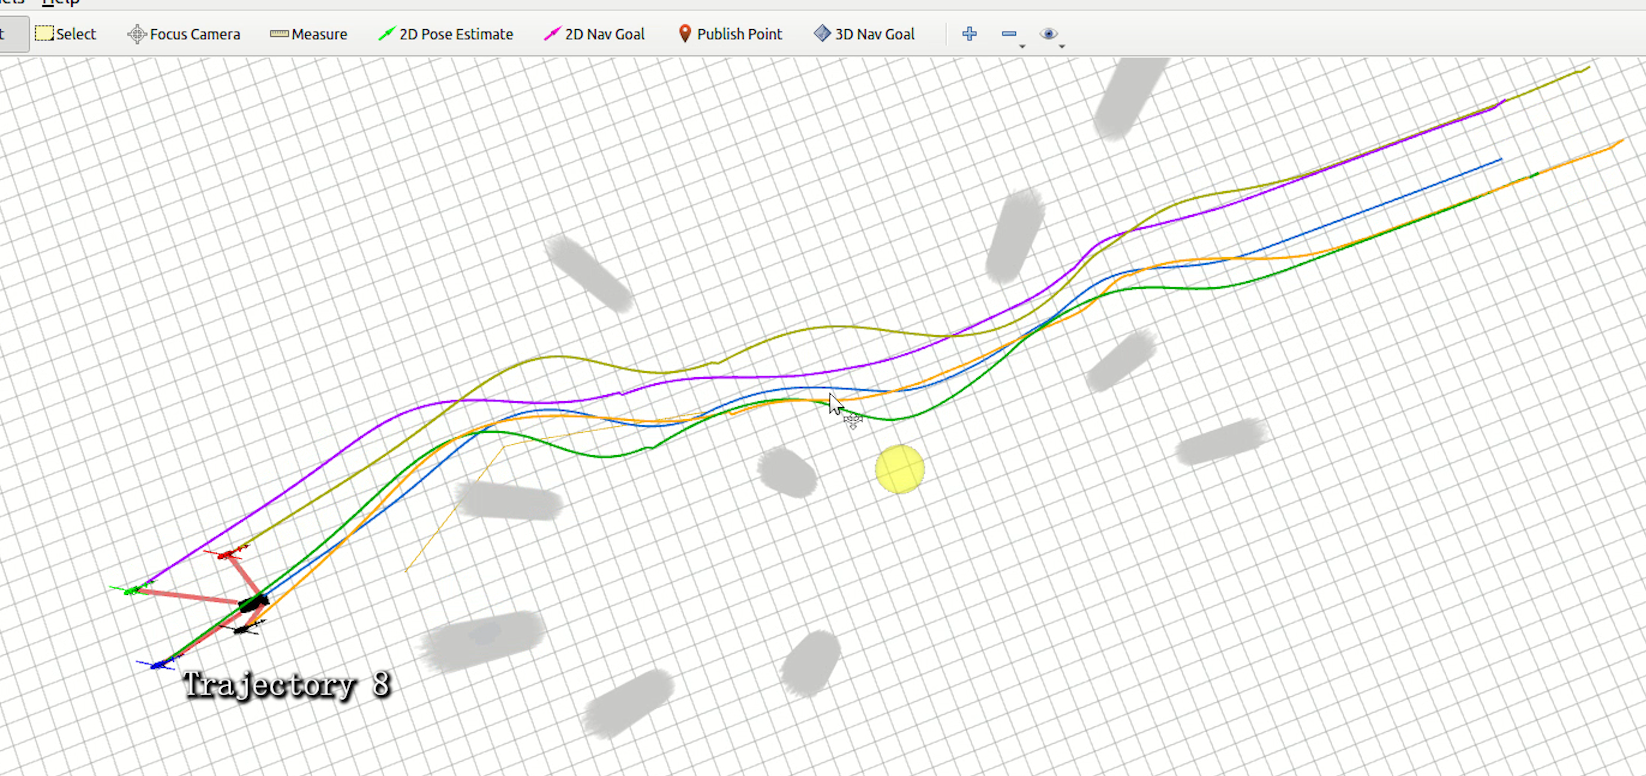
\includegraphics[width = 0.45\textwidth]{fig/figure_chap6/rigid_trajectory/8.png}}\\
    \caption{刚体吊挂物协同吊挂系统避障轨迹\label{rigid_trajectory}}
\end{figure}

\begin{figure}[htb!]
    \centering
    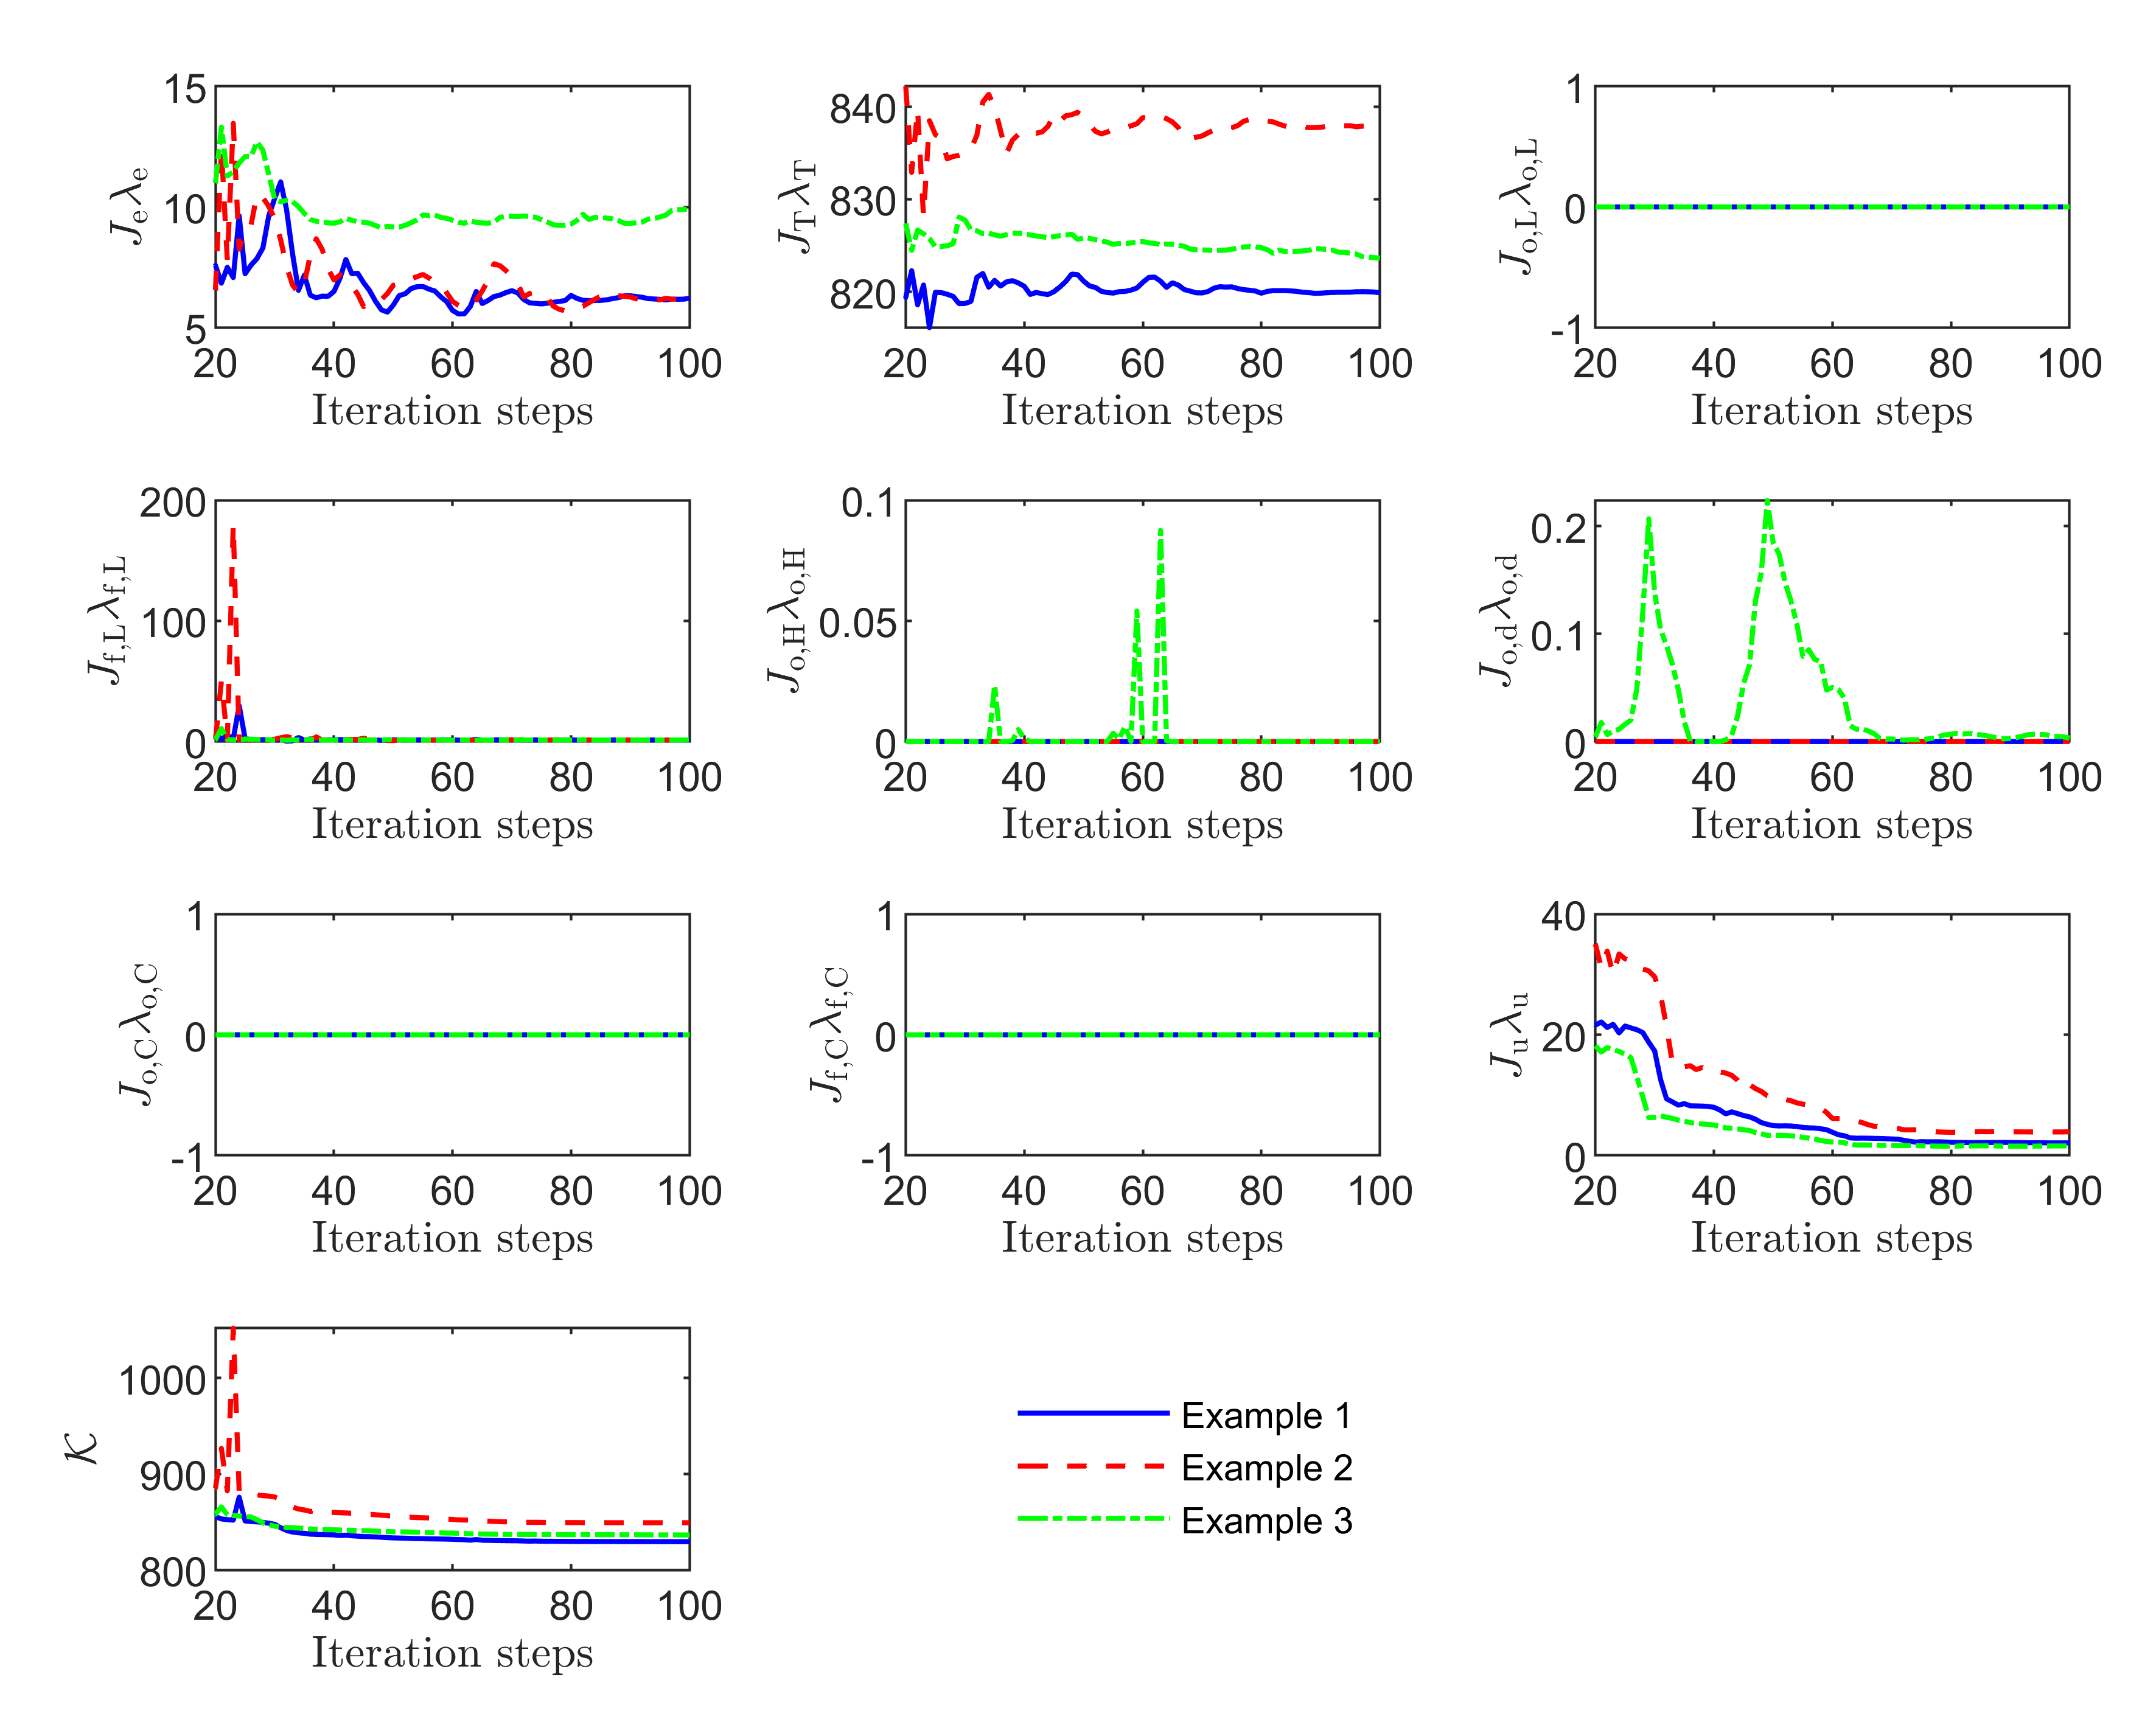
\includegraphics{fig/figure_chap6/cost_rigid.png}
    \caption{刚体吊挂物协同吊挂系统代价函数随迭代步数的变化\label{rigid_cost}}
\end{figure}

\begin{figure}[htb!]
    \centering
    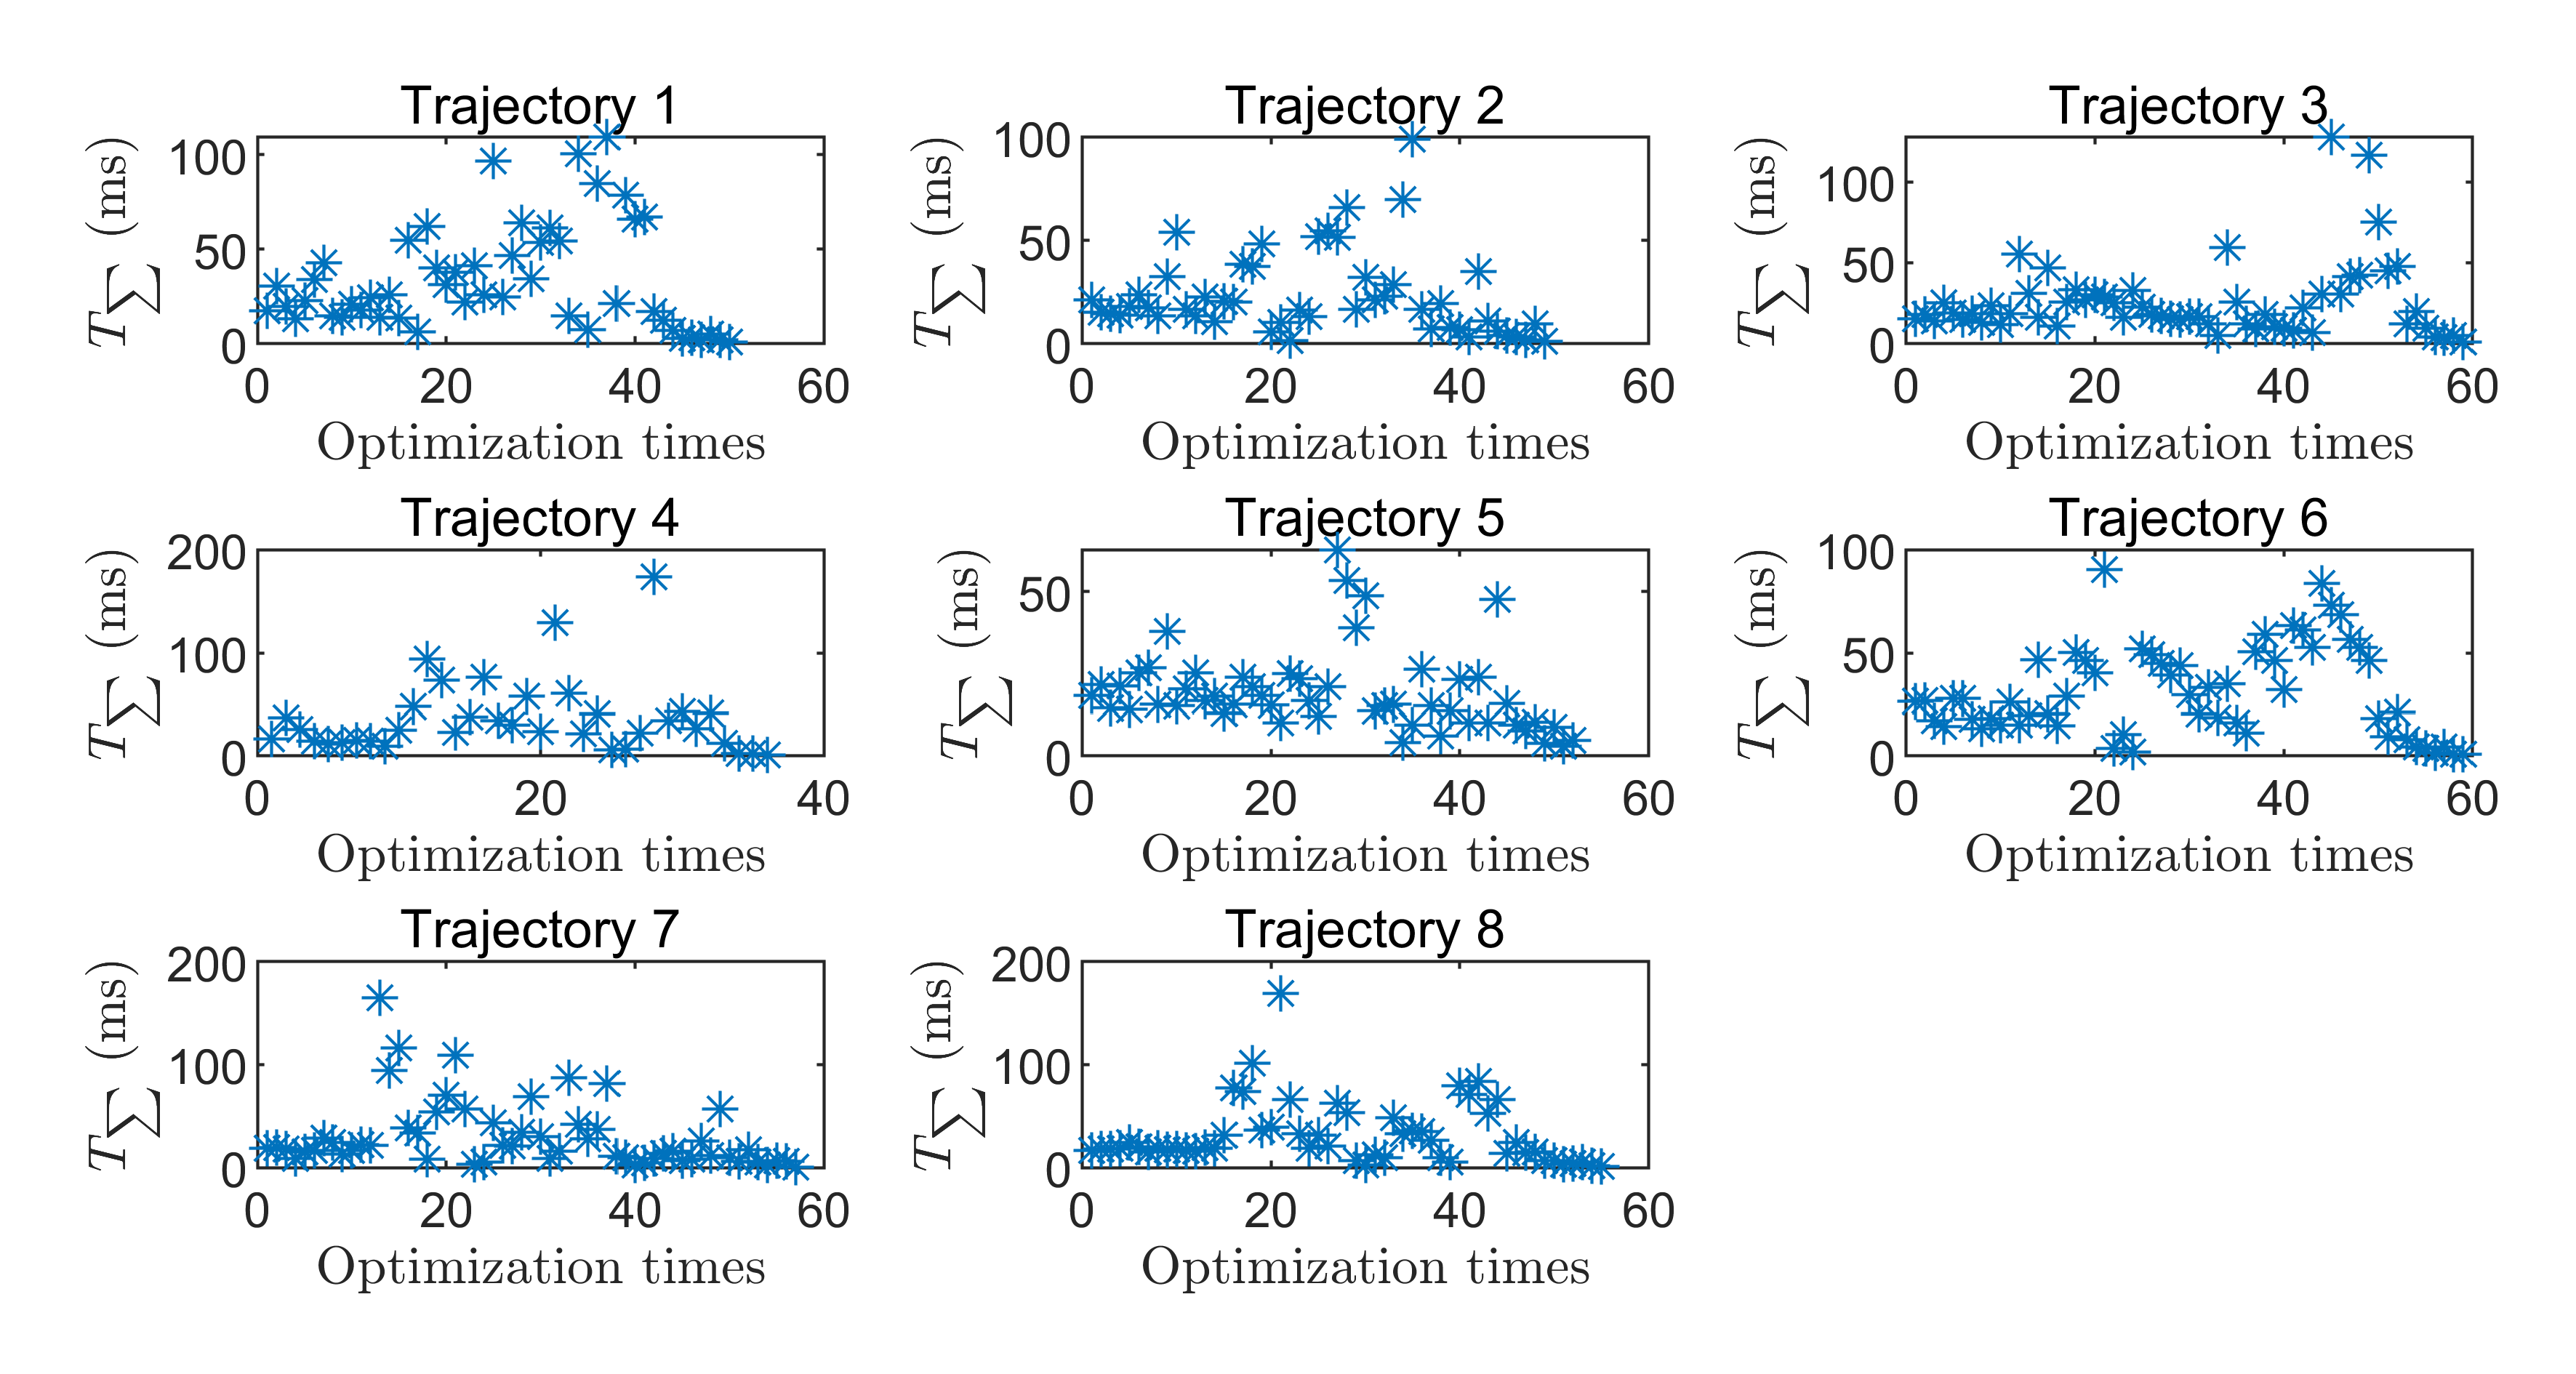
\includegraphics[width = \textwidth]{fig/figure_chap6/time_rigid.png}
    \caption{刚体吊挂物协同吊挂系统迭代收敛时间\label{rigid_time}}
\end{figure}

图\ref{rigid_trajectory}给出了吊挂物建模为刚体时的避障仿真结果。与吊挂物建模为质点时类似,8个地图是随机生成的。相关视频见链接\href{https://www.bilibili.com/video/BV1VP4y1y7K6/}{https://www.bilibili.com/video/BV1VP4y1y7K6/}。可以看出,尽管吊挂物建模为刚体时总时间惩罚权重$\lambda_{\rm{e}}$较大,直升机1到4的机动性没有太大的区别。这与上述分析相同,是因为吊挂物建模为刚体时各吊索力均直接承担吊挂物的加速运动。此外,从图\ref{rigid_trajectory}和视频链接均可看出,吊挂物、直升机、吊索距离障碍物均有一定的安全距离、直升机间没有相互碰撞、吊索没有交叉。

进而,值得注意的是,轨迹3后半段由于障碍物密集,本文提出的基于微分平坦输出和minco的避障优化算法不能求出可行解。参考图\ref{obstacle_sim}可知,此时会再次调用$\rm{A}^\star$算法计算初始轨迹,为本文提出的优化算法提供初值。从仿真结果可知,上述策略是可行的。

从上述8条轨迹优化过程中随机选取3次迭代,图\ref{rigid_cost}详细给出了各惩罚函数随迭代步数的变化。与图\ref{point_cost}结果类似,各惩罚项随迭代步数逐渐收敛,验证了所提优化算法的有效性。

对应图\ref{rigid_trajectory}中的8条避障轨迹,图\ref{rigid_time}给出了每条轨迹每次迭代消耗的时间。可见,97.36\%的迭代消耗时间均小于100 ms,8条轨迹共417次迭代平均每次迭代优化时间为28.68 ms,满足实时性要求。

\section{本章小结}\label{Section6:conclusion}
本章提出了基于微分平坦输出和minco的直升机协同吊挂系统实时避障轨迹规划策略:
\begin{enumerate}
    \item 分析了考虑吊索力的直升机微分平坦特性,针对吊挂物建模为质点和刚体两种情况,给出了协同吊挂系统的微分平坦输出,推导了其微分平坦映射。
    \item 基于直升机协同吊挂系统微分平坦特性和minco轨迹表示方法,以最小化轨迹能量和轨迹总消耗时间为目的,针对吊挂物建模为质点和刚体两种情况,将协同吊挂系统避障问题转换为无约束优化问题处理,考虑了吊挂物避障、吊挂物状态量可行性、直升机避障、直升机间避免相互碰撞、吊索避障、吊索力可行性、控制点均匀分布惩罚项。
    \item 基于本文提出的避障优化算法,以四直升机协同吊挂为例,分吊挂物建模为质点和刚体两种情况开展了仿真。仿真结果验证了本文所提避障优化算法的有效性、可行性和实时性。
    \item 仿真发现,由于微分平坦输出不同,吊挂物建模为质点时直升机1相比其他直升机机动性更大,吊挂物建模为刚体时各直升机具有相似的机动特性,从安全角度考虑,基于本文所提避障优化算法,吊挂物建模为刚体时效果更佳。
\end{enumerate}

需要说明的是,本文所提算法具有较强的可实现性,目前基于MavRos(Mavlink+Ros),开源飞控与Ros之间的交互已经比较成熟,基于本文所提优化算法发布的避障轨迹,可以直接通过Mavros发送给直升机飞控。后续工作计划开展基于本文所提避障优化算法的试验试飞工作。
